  \item $\mathrm{MgSO}_{4}$ suyuqlanmasi elektroliz qilinganda anodda qanday modda(lar) ajralib chiqadi?\\
A) S\\
B) Mg\\
C) $\mathrm{O}_{2}$\\
D) $\mathrm{H}_{2}$
  \item $\mathrm{Na}_{2} \mathrm{~S}$ suyuqlanmasi elektroliz qilinganda anodda qanday modda(lar) ajralib chiqadi?\\
A) S\\
B) Na\\
C) $\mathrm{O}_{2}$\\
D) $\mathrm{H}_{2}$
  \item $\mathrm{K}_{2} \mathrm{SO}_{4}$ suyuqlanmasi elektroliz qilinganda anodda qanday modda(lar) ajralib chiqadi?\\
A) $\mathrm{Cl}_{2}$\\
B) K\\
C) $\mathrm{O}_{2}$\\
D) $\mathrm{H}_{2}$
  \item NaI suyuqlanmasi elektroliz qilinganda anodda qanday modda(lar) ajralib chiqadi?\\
A) $\mathrm{I}_{2}$\\
B) Na\\
C) $\mathrm{O}_{2}$\\
D) $\mathrm{H}_{2}$
  \item NaCl suyuqlanmasi elektroliz qilinganda katodda qanday modda(lar) ajralib chiqadi?\\
A) $\mathrm{Cl}_{2}$\\
B) Na\\
C) $\mathrm{O}_{2}$\\
D) $\mathrm{H}_{2}$
  \item $\mathrm{AlCl}_{3}$ suyuqlanmasi elektroliz qilinganda katodda qanday modda(lar) ajralib chiqadi?\\
A) $\mathrm{Cl}_{2}$\\
B) Na\\
C) $\mathrm{O}_{2}$\\
D) Al
  \item $\mathrm{K}_{2} \mathrm{CO}_{3}$ suyuqlanmasi elektroliz qilinganda katodda qanday modda(lar) ajralib chiqadi?\\
A) C\\
B) K\\
C) $\mathrm{O}_{2}$\\
D) $\mathrm{H}_{2}$
  \item $\mathrm{CuCl}_{2}$ suyuqlanmasi elektroliz qilinganda katodda qanday modda(lar) ajralib chiqadi?\\
A) $\mathrm{Cl}_{2}$\\
B) $\mathrm{Cu}_{2} \mathrm{O}$\\
C) $\mathrm{O}_{2}$\\
D) Cu
  \item $\mathrm{FeCl}_{2}$ suyuqlanmasi elektroliz qilinganda katodda qanday modda(lar) ajralib chiqadi?\\
A) Fe\\
B) $\mathrm{Fe}_{2} \mathrm{O}_{3}$\\
C) $\mathrm{O}_{2}$\\
D) $\mathrm{H}_{2}$
  \item $\mathrm{CuSO}_{4}$ ning eritmasi elektroliz qilinganda katodda qanday modda(lar) ajralib chiqadi?\\
A) $\mathrm{Cl}_{2}$\\
B) $\mathrm{Cu}_{2} \mathrm{O}$\\
C) $\mathrm{O}_{2}$\\
D) Cu
  \item $\mathrm{AuCl}_{3}$ ning eritmasi elektroliz qilinganda katodda qanday modda(lar) ajralib chiqadi?\\
A) $\mathrm{Cl}_{2}$\\
B) Au\\
C) $\mathrm{O}_{2}$\\
D) $\mathrm{H}_{2}$
  \item NaCl ning eritmasi elektroliz qilinganda katodda qanday modda(lar) ajralib chiqadi?\\
A) $\mathrm{Cl}_{2}$\\
B) Na\\
C) $\mathrm{O}_{2}$\\
D) $\mathrm{H}_{2}$
  \item $\mathrm{FeSO}_{4}$ ning eritmasi elektroliz qilinganda katodda qanday modda(lar) ajralib chiqadi?\\
A) Fe\\
B) $\mathrm{Fe}, \mathrm{H}_{2}$\\
C) $\mathrm{H}_{2}$\\
D) $\mathrm{Fe}_{2} \mathrm{O}_{3}$
  \item $\mathrm{K}_{2} \mathrm{CO}_{3}$ ning eritmasi elektroliz qilinganda katodda qanday modda(lar) ajralib chiqadi?\\
A) $\mathrm{Cl}_{2}$\\
B) $\mathrm{K}, \mathrm{H}_{2}$\\
C) $\mathrm{O}_{2}$\\
D) $\mathrm{H}_{2}$
  \item $\mathrm{CuSO}_{4}$ ning eritmasi elektroliz qilinganda anodda qanday modda(lar) ajralib chiqadi?\\
A) $\mathrm{Cl}_{2}$\\
B) $\mathrm{Cu}_{2} \mathrm{O}$\\
C) $\mathrm{O}_{2}$\\
D) Cu
  \item $\mathrm{AuCl}_{3}$ ning eritmasi elektroliz qilinganda anodda qanday modda(lar) ajralib chiqadi?\\
A) $\mathrm{Cl}_{2}$\\
B) Au\\
C) $\mathrm{O}_{2}$\\
D) $\mathrm{Au}_{2} \mathrm{O}_{3}$
  \item $\mathrm{FeSO}_{4}$ ning eritmasi elektroliz qilinganda anodda qanday modda(lar) ajralib chiqadi?\\
A) S\\
B) Fe\\
C) $\mathrm{O}_{2}$\\
D) $\mathrm{SO}_{2}$
  \item NaF ning eritmasi elektroliz qilinganda anodda qanday modda(lar) ajralib chiqadi?\\
A) $\mathrm{F}_{2}$\\
B) Na\\
C) $\mathrm{O}_{2}$\\
D) $\mathrm{H}_{2}$
  \item $\mathrm{K}_{2} \mathrm{SO}_{4}$ ning eritmasi elektroliz qilinganda anodda qanday modda(lar) ajralib chiqadi?\\
A) S\\
B) K\\
C) $\mathrm{O}_{2}$\\
D) $\mathrm{SO}_{2}$
  \item $\mathrm{CuSO}_{4}$ ning mo'l miqdordagi eritmasi orqali 3 F miqdorida elektr toki o'tkazilganda katodda necha g metall ajralib chiqadi?\\
A) 96\\
B) 32\\
C) 64\\
D) 16\\
  \item $\mathrm{AuCl}_{3}$ ning mo'l miqdordagi eritmasi orqali 6 F miqdorida elektr toki o'tkazilganda katodda necha g metall ajralib chiqadi?\\
A) 591\\
B) 197\\
C) 394\\
D) 98
  \item $\mathrm{Hg}\left(\mathrm{NO}_{3}\right)_{2}$ ning mo'l miqdordagi eritmasi orqali 2 F miqdorida elektr toki o'tkazilganda katodda necha g metall ajralib chiqadi?\\
A) 402\\
B) 150\\
C) 100,5\\
D) 201
  \item $\mathrm{Al}_{2}\left(\mathrm{SO}_{4}\right)_{3}$ ning mo'l miqdordagi eritmasi orqali 3 F miqdorida elektr toki o'tkazilganda katodda necha g metall ajralib chiqadi?\\
A) 27\\
B) 54\\
C) 9\\
D) 18
  \item $\mathrm{CuCl}_{2}$ ning mo'l miqdordagi eritmasi orqali 4 F miqdorida elektr toki o'tkazilganda katodda necha g metall ajralib chiqadi?\\
A) 96\\
B) 128\\
C) 64\\
D) 32
  \item $\mathrm{CuSO}_{4}$ ning mo'l miqdordagi eritmasi orqali 3 F miqdorida elektr toki o'tkazilganda anodda necha g metalmas ajralib chiqadi?\\
A) 8\\
B) 32\\
C) 24\\
D) 16
  \item $\mathrm{AuCl}_{3}$ ning mo'l miqdordagi eritmasi orqali 6 F miqdorida elektr toki o'tkazilganda anodda necha g metalmas ajralib chiqadi?\\
A) 213\\
B) 142\\
C) 71\\
D) 35,5
  \item $\mathrm{Hg}\left(\mathrm{NO}_{3}\right)_{2}$ ning mo'l miqdordagi eritmasi orqali 2 F miqdorida elektr toki o'tkazilganda anodda necha g metalmas ajralib chiqadi?\\
A) 8\\
B) 32\\
C) 24\\
D) 16
  \item $\mathrm{Al}_{2}\left(\mathrm{SO}_{4}\right)_{3}$ ning mo'l miqdordagi eritmasi orqali 3 F miqdorida elektr toki o'tkazilganda anodda necha g metalmas ajralib chiqadi?\\
A) 8\\
B) 32\\
C) 24\\
D) 16
  \item $\mathrm{CuCl}_{2}$ ning mo'l miqdordagi eritmasi orqali 4 F miqdorida elektr toki\\
o'tkazilganda anodda necha g metalmas ajralib chiqadi?\\
A) 213\\
B) 142\\
C) 71\\
D) 35,5
  \item Tarkibida $3 \mathrm{~mol} \mathrm{CuSO}_{4}$ saqlagan eritma orqali 7 F miqdorida elektr toki o'tkazilganda katodda (inert elektrod) necha g modda(lar) ajralib chiqadi?\\
A) 193\\
B) 64\\
C) 192\\
D) 97
  \item Tarkibida 2 mol NaCl saqlagan eritma orqali 4 F miqdorida elektr toki o'tkazilganda katodda (inert elektrod) necha g modda(lar) ajralib chiqadi?\\
A) 3\\
B) 4\\
C) 2\\
D) 6
  \item Tarkibida $2 \mathrm{~mol} \mathrm{AgNO}_{3}$ saqlagan eritma orqali 3 F miqdorida elektr toki o'tkazilganda katodda (inert elektrod) necha g modda(lar) ajralib chiqadi?\\
A) 108\\
B) 216\\
C) 54\\
D) 217
  \item Tarkibida $2 \mathrm{~mol} \mathrm{Fe}\left(\mathrm{NO}_{3}\right)_{3}$ saqlagan eritma orqali 7 F miqdorida elektr toki o'tkazilganda katodda (inert elektrod) necha g modda(lar) ajralib chiqadi?\\
A) 112\\
B) 56\\
C) 113\\
D) 28
  \item Tarkibida 1 mol NaI saqlagan eritma orqali 5 F miqdorida elektr toki o'tkazilganda katodda (inert elektrod) necha g modda(lar) ajralib chiqadi?\\
A) 27\\
B) 5\\
C) 1\\
D) 23
  \item Tarkibida $2 \mathrm{~mol} \mathrm{CuSO}_{4}$ saqlagan eritma orqali 2 F miqdorida elektr toki o'tkazilganda anodda (inert elektrod) necha g modda(lar) ajralib chiqadi?\\
A) 8\\
B) 16\\
C) 32\\
D) 24
  \item Tarkibida $1 \mathrm{~mol} \mathrm{Al}_{2}\left(\mathrm{SO}_{4}\right)_{3}$ saqlagan eritma orqali 5 F miqdorida elektr toki o'tkazilganda anodda (inert elektrod) necha g modda(lar) ajralib chiqadi?\\
A) 40\\
B) 64\\
C) 36\\
D) 32
  \item Tarkibida $2 \mathrm{~mol} \mathrm{CdSO}_{4}$ saqlagan eritma orqali 3 F miqdorida elektr toki o'tkazilganda anodda (inert elektrod) necha g modda(lar) ajralib chiqadi?\\
A) 8\\
B) 16\\
C) 32\\
D) 24
  \item Tarkibida 3 mol NaBr saqlagan eritma orqali 2 F miqdorida elektr toki o'tkazilganda anodda (inert elektrod) necha g modda(lar) ajralib chiqadi?\\
A) 2\\
B) 46\\
C) 160\\
D) 80
  \item Tarkibida $2 \mathrm{~mol} \mathrm{Cu}\left(\mathrm{NO}_{3}\right)_{2}$ saqlagan eritma orqali 3 F miqdorida elektr toki o'tkazilganda anodda (inert elektrod) necha g modda(lar) ajralib chiqadi?\\
A) 8\\
B) 16\\
C) 32\\
D) 24
  \item Kulonometrda tarkibida $0,5 \mathrm{~mol}$ $\mathrm{CuSO}_{4}$ saqlagan eritma orqali 193000 kulon miqdorida elektr toki o'tkazilganda katodda (inert elektrod) necha g modda(lar) ajralib chiqadi?\\
A) 33\\
B) 64\\
C) 65\\
D) 97
  \item Kulonometrda tarkibida $1 \mathrm{~mol} \mathrm{AgNO}_{3}$ saqlagan eritma orqali 289500 kulon miqdorida elektr toki o'tkazilganda katodda (inert elektrod) necha g modda(lar) ajralib chiqadi?\\
A) 108\\
B) 54\\
C) 110\\
D) 216
  \item Kulonometrda tarkibida $0,5 \mathrm{~mol} \mathrm{NaCl}$ saqlagan eritma orqali 96500 kulon miqdorida elektr toki o'tkazilganda katodda (inert elektrod) necha g modda(lar) ajralib chiqadi?\\
A) 12,5\\
B) 1\\
C) 3\\
D) 2
  \item Kulonometrda tarkibida 1 mol $\mathrm{Cd}\left(\mathrm{NO}_{3}\right)_{2}$ saqlagan eritma orqali 193000 kulon miqdorida elektr toki o'tkazilganda katodda (inert elektrod) necha g modda(lar) ajralib chiqadi?\\
A) 28\\
B) 56\\
C) 224\\
D) 112
  \item Kulonometrda tarkibida $0,5 \mathrm{~mol} \mathrm{CoCl}_{2}$ saqlagan eritma orqali 96500 kulon miqdorida elektr toki o'tkazilganda katodda (inert elektrod) necha g modda(lar) ajralib chiqadi?\\
A) 24,5\\
B) 118\\
C) 59\\
D) 29
  \item Kulonometrda tarkibida $0,5 \mathrm{~mol}$ $\mathrm{Cu}\left(\mathrm{NO}_{3}\right)_{2}$ saqlagan eritma orqali 193000 kulon miqdorida elektr toki o'tkazilganda anodda (inert elektrod) necha g modda(lar) ajralib chiqadi?\\
A) 24\\
B) 8\\
C) 32\\
D) 16
  \item Kulonometrda tarkibida $0,5 \mathrm{~mol}$ $\mathrm{AgNO}_{3}$ saqlagan eritma orqali 96500 kulon miqdorida elektr toki o'tkazilganda anodda (inert elektrod) necha g modda(lar) ajralib chiqadi?\\
A) 24\\
B) 8\\
C) 32\\
D) 16
  \item Kulonometrda tarkibida $1,5 \mathrm{~mol} \mathrm{NaCl}$ saqlagan eritma orqali 193000 kulon miqdorida elektr toki o'tkazilganda anodda (inert elektrod) necha g modda(lar) ajralib chiqadi?\\
A) 57,25\\
B) 53,25\\
C) 8\\
D) 16
  \item Kulonometrda tarkibida $0,5 \mathrm{~mol}$ KI saqlagan eritma orqali 193000 kulon miqdorida elektr toki o'tkazilganda anodda(inert elektrod) necha g modda(lar) ajralib chiqadi?\\
A) 16\\
B) 8\\
C) 75,5\\
D) 63,5
  \item Kulonometrda tarkibida $0,5 \mathrm{~mol}$ $\mathrm{Fe}\left(\mathrm{NO}_{3}\right)_{3}$ saqlagan eritma orqali 193000 kulon miqdorida elektr toki o'tkazilganda\\
anodda(inert elektrod) necha g modda(lar) ajralib chiqadi?\\
A) 72\\
B) 64\\
C) 16\\
D) 97
  \item $0,2 \mathrm{~mol} \mathrm{CuSO}_{4}, 0,2 \mathrm{~mol} \mathrm{AgNO}_{3}$, va 0.2 $\mathrm{mol} \mathrm{AuCl}_{3}$ saqlagan eritma orqali 1 F tok o'tkazildi. Katodda ajralgan metallarning massasini (g) aniqlang.\\
A) $\mathrm{Cu}-6,4 ; \mathrm{Ag}-21,6 ; \mathrm{Au}-39,4$\\
B) $\mathrm{Cu}-3,2 ; \mathrm{Ag}-21,6 ; \mathrm{Au}-19,7$\\
C) $\mathrm{Cu}-6,4 ; \mathrm{Ag}-10,8 ; \mathrm{Au}-39,4$\\
D) $\mathrm{Cu}-12,8 ; \mathrm{Ag}-21,6 ; \mathrm{Au}-19,7$\\
  \item $0,3 \mathrm{~mol} \mathrm{CuSO}_{4}, 0,3 \mathrm{~mol} \mathrm{AgNO}_{3}$, va 0.1 $\mathrm{mol} \mathrm{AuCl}_{3}$ saqlagan eritma orqali 1 F tok o'tkazildi. Katodda ajralgan metallarning massasini (g) aniqlang.\\
A) $\mathrm{Cu}-12,8 ; \mathrm{Ag}-21,6 ; \mathrm{Au}-39,4$\\
B) $\mathrm{Cu}-3,2 ; \mathrm{Ag}-21,6 ; \mathrm{Au}-19,7$\\
C) $\mathrm{Cu}-12,8 ; \mathrm{Ag}-32,4 ; \mathrm{Au}-19,7$\\
D) $\mathrm{Cu}-12,8 ; \mathrm{Ag}-21,6 ; \mathrm{Au}-19,7$
  \item $0,2 \mathrm{~mol} \mathrm{CuSO}_{4}, 0,2 \mathrm{~mol} \mathrm{AgNO}_{3}$, va 0.3 mol $\mathrm{AuCl}_{3}$ saqlagan eritma orqali $1,4 \mathrm{~F}$ tok o'tkazildi. Katodda ajralgan metallarning massasini ( g ) aniqlang.\\
A) $\mathrm{Cu}-9,6 ; \mathrm{Ag}-21,6 ; \mathrm{Au}-39,4$\\
B) $\mathrm{Cu}-12,8 ; \mathrm{Ag}-21,6 ; \mathrm{Au}-19,7$\\
C) $\mathrm{Cu}-6,4 ; \mathrm{Ag}-10,8 ; \mathrm{Au}-59,1$\\
D) $\mathrm{Cu}-9,6 ; \mathrm{Ag}-21,6 ; \mathrm{Au}-59,1$
  \item $0,2 \mathrm{~mol} \mathrm{CuSO}_{4}, 0,4 \mathrm{~mol} \mathrm{AgNO}_{3}$, va 0.2 mol $\mathrm{AuCl}_{3}$ saqlagan eritma orqali $1,2 \mathrm{~F}$ tok o'tkazildi. Katodda ajralgan metallarning massasini (g) aniqlang.\\
A) $\mathrm{Cu}-6,4 ; \mathrm{Ag}-43,2 ; \mathrm{Au}-39,4$\\
B) $\mathrm{Cu}-3,2 ; \mathrm{Ag}-21,6 ; \mathrm{Au}-19,7$\\
C) $\mathrm{Cu}-12,8 ; \mathrm{Ag}-43,2 ; \mathrm{Au}-39,4$\\
D) $\mathrm{Cu}-12,8 ; \mathrm{Ag}-21,6 ; \mathrm{Au}-19,7$
  \item $0,1 \mathrm{~mol} \mathrm{CuSO}_{4}, 0,4 \mathrm{~mol} \mathrm{AgNO}_{3}$, va 0.2 $\mathrm{mol} \mathrm{AuCl}_{3}$ saqlagan eritma orqali $1,1 \mathrm{~F}$ tok o'tkazildi. Katodda ajralgan metallarning massasini (g) aniqlang.\\
A) $\mathrm{Cu}-6,4 ; \mathrm{Ag}-21,6 ; \mathrm{Au}-39,4$\\
B) $\mathrm{Cu}-3,2 ; \mathrm{Ag}-21,6 ; \mathrm{Au}-39,4$\\
C) $\mathrm{Cu}-3,2 ; \mathrm{Ag}-43,2 ; \mathrm{Au}-39,4$\\
D) $\mathrm{Cu}-12,8 ; \mathrm{Ag}-21,6 ; \mathrm{Au}-19,7$
  \item $0,8 \mathrm{~mol} \mathrm{CuSO}_{4}, 0,1 \mathrm{~mol} \mathrm{AgNO}_{3}$, va 0.1 $\mathrm{mol} \mathrm{AuCl}_{3}$ saqlagan eritma orqali 1 F tok o'tkazildi. Katodda ajralgan metallarning massasini ( g ) aniqlang.\\
A) $\mathrm{Cu}-6,4 ; \mathrm{Ag}-21,6 ; \mathrm{Au}-39,4$\\
B) $\mathrm{Cu}-19,2 ; \mathrm{Ag}-10,8 ; \mathrm{Au}-19,7$\\
C) $\mathrm{Cu}-6,4 ; \mathrm{Ag}-10,8 ; \mathrm{Au}-39,4$\\
D) $\mathrm{Cu}-19,2 ; \mathrm{Ag}-21,6 ; \mathrm{Au}-19,7$
  \item $0,3 \mathrm{~mol} \mathrm{CuSO}_{4}, 0,3 \mathrm{~mol} \mathrm{AgNO}_{3}$, va 0.3 mol $\mathrm{AuCl}_{3}$ saqlagan eritma orqali $1,5 \mathrm{~F}$ tok o'tkazildi. Katodda ajralgan metallarning massasini (g) aniqlang.\\
A) $\mathrm{Cu}-9,6 ; \mathrm{Ag}-32,4 ; \mathrm{Au}-59,1$\\
B) $\mathrm{Cu}-3,2 ; \mathrm{Ag}-21,6 ; \mathrm{Au}-19,7$\\
C) $\mathrm{Cu}-6,4 ; \mathrm{Ag}-10,8 ; \mathrm{Au}-59,1$\\
D) $\mathrm{Cu}-9,6 ; \mathrm{Ag}-21,6 ; \mathrm{Au}-19,7$
  \item $0,5 \mathrm{~mol} \mathrm{CuSO}_{4}, 0,4 \mathrm{~mol} \mathrm{AgNO}_{3}$, va 0.1 mol $\mathrm{AuCl}_{3}$ saqlagan eritma orqali $1,2 \mathrm{~F}$ tok o'tkazildi. Katodda ajralgan metallarning massasini (g) aniqlang.\\
A) $\mathrm{Cu}-16 ; \mathrm{Ag}-21,6 ; \mathrm{Au}-19,7$\\
B) $\mathrm{Cu}-3,2 ; \mathrm{Ag}-21,6 ; \mathrm{Au}-19,7$\\
C) $\mathrm{Cu}-16 ; \mathrm{Ag}-43,2 ; \mathrm{Au}-19,7$\\
D) $\mathrm{Cu}-12,8 ; \mathrm{Ag}-21,6 ; \mathrm{Au}-19,7$
  \item $0,25 \mathrm{~mol} \mathrm{CuSO}_{4}, 0,3 \mathrm{~mol} \mathrm{AgNO}_{3}$, va 0.1 $\mathrm{mol} \mathrm{AuCl}_{3}$ saqlagan eritma orqali 1 F tok o'tkazildi. Katodda ajralgan metallarning massasini ( g ) aniqlang.\\
A) $\mathrm{Cu}-6,4 ; \mathrm{Ag}-21,6 ; \mathrm{Au}-39,4$\\
B) $\mathrm{Cu}-3,2 ; \mathrm{Ag}-21,6 ; \mathrm{Au}-19,7$\\
C) $\mathrm{Cu}-6,4 ; \mathrm{Ag}-10,8 ; \mathrm{Au}-39,4$\\
D) $\mathrm{Cu}-12,8 ; \mathrm{Ag}-32,4 ; \mathrm{Au}-19,7$
  \item $0,3 \mathrm{~mol} \mathrm{CuSO}_{4}, 0,5 \mathrm{~mol} \mathrm{AgNO}_{3}$, va 0.1 $\mathrm{mol} \mathrm{AuCl}_{3}$ saqlagan eritma orqali $1,2 \mathrm{~F}$ tok o'tkazildi. Katodda ajralgan metallarning massasini (g) aniqlang.\\
A) $\mathrm{Cu}-6,4 ; \mathrm{Ag}-21,6 ; \mathrm{Au}-39,4$\\
B) $\mathrm{Cu}-12,8 ; \mathrm{Ag}-54 ; \mathrm{Au}-19,7$\\
C) $\mathrm{Cu}-6,4 ; \mathrm{Ag}-54 ; \mathrm{Au}-39,4$\\
D) $\mathrm{Cu}-12.8 ; \mathrm{Ag}-21.6 ; \mathrm{Au}-19,7$
  \item $\mathrm{AgNO}_{3}$ ning mo'l miqdordagi eritmasidan 8 soat davomida $2,68 \mathrm{~A}$ kuchga ega bo'lgan tok o'tkazildi. Katodda(inert elektrod) ajralib chiqqan kumushning massasini (g) aniqlang.\\
A) 86,4\\
B) 10,8\\
C) 21,6\\
D) 32,4 
  \item $\mathrm{CuSO}_{4}$ ning mo'l miqdordagi eritmasidan 5 soat davomida $13,4 \mathrm{~A}$ kuchga ega bo'lgan tok o'tkazildi. Katodda (inert elektrod) ajralib chiqqan misning massasini (g) aniqlang.\\
A) 32\\
B) 64\\
C) 48\\
D) 80
  \item $\mathrm{AuCl}_{3}$ ning mo'l miqdordagi eritmasidan 3 soat davomida 2,68 A kuchga ega bo'lgan tok o'tkazildi. Katodda (inert elektrod) ajralib chiqqan oltinning massasini (g) aniqlang.\\
A) 197\\
B) 65,67\\
C) 19,7\\
D) 39,4
  \item KOH ning mo'l miqdordagi eritmasidan 4 soat davomida 6,7 A kuchga ega bo'lgan tok o'tkazildi. Katodda (inert elektrod) ajralib chiqqan moddaning massasini (g) aniqlang.\\
A) 9\\
B) 1\\
C) 39\\
D) 40
  \item $\mathrm{NiCl}_{2}$ ning mo'l miqdordagi eritmasidan 2 soat davomida $13,4 \mathrm{~A}$ kuchga ega bo'lgan tok o'tkazildi. Katodda (inert elektrod) ajralib chiqqan nikelning massasini (g) aniqlang.\\
A) 59\\
B) 118\\
C) 29,5\\
D) 5,9
  \item $\mathrm{HNO}_{3}$ ning mo'l miqdordagi eritmasidan 4 soat davomida 6,7 A kuchga ega bo'lgan tok o'tkazildi. Anodda (inert elektrod) ajralib chiqqan moddaning massasini (g) aniqlang.\\
A) 8\\
B) 16\\
C) 32\\
D) 3,2
  \item $\mathrm{KNO}_{3}$ ning mo'l miqdordagi eritmasidan 10 soat davomida $2,68 \mathrm{~A}$ kuchga ega bo'lgan tok o'tkazildi. Anodda\\
(inert elektrod) ajralib chiqqan moddaning massasini (g) aniqlang.\\
A) 8\\
B) 16\\
C) 32\\
D) 3,2
  \item $\mathrm{Cu}\left(\mathrm{NO}_{3}\right)_{-2}$ ning mo'l miqdordagí eritmasidan 4 soat davomida 13.4 A kuchga ega bo'lgan tok o'tkazildi. Anodda (inert elektrod) ajralib chiqqan moddaning massasini (g) aniqlang.\\
A) 8\\
B) 16\\
C) 32\\
D) 3,2
  \item NaCl ning mo'l miqdordagi eritmasidan 4 soat davomida 13,4 A kuchga ega bo'lgan tok o'tkazildi. Anodda (inert elektrod) ajralib chiqqan moddaning massasini ( g ) aniqlang.\\
A) 46\\
B) 2\\
C) 71\\
D) 35,5
  \item KI ning mo'l miqdordagi eritmasidan 4 soat davomida $6,7 \mathrm{~A}$ kuchga ega bo'lgan tok o'tkazildi. Anodda (inert elektrod) ajralib chiqqan moddaning massasini (g) aniqlang.\\
A) 254\\
B) 25,4\\
C) 127\\
D) 12,7
  \item $\mathrm{CuSO}_{4}$ eritmasini necha minut $16,08 \mathrm{~A}$ tok bilan elektroliz qilinsa, katodda (inert elektrod) 32 g metall ajralib chiqadi?\\
A) 100\\
B) 200\\
C) 50\\
D) 60\\
  \item $\mathrm{AgNO}_{3}$ eritmasini necha minut $32,16 \mathrm{~A}$ tok bilan elektroliz qilinsa, katodda (inert elektrod) 54 g metall ajralib chiqadi?\\
A) 10\\
B) 20\\
C) 50\\
D) 25
  \item $\mathrm{NiCl}_{2}$ eritmasini necha minut $64,32 \mathrm{~A}$ tok bilan elektroliz qilinsa, katodda (inert elektrod) 59 g metall ajralib chiqadi?\\
A) 100\\
B) 200\\
C) 50\\
D) 60
  \item $\mathrm{MnSO}_{4}$ eritmasini necha minut $16,08 \mathrm{~A}$ tok bilan elektroliz qilinsa, katodda (inert elektrod) 110 g metall ajralib chiqadi?\\
A) 200\\
B) 400\\
C) 150\\
D) 160
  \item KI oritmanini nochn minut $64,32 \Lambda$ tok bilan olektroliz qilines, anoddn inor't olok(rod) $254 \mathrm{~g} l_{2}$ njralib chiqndi?\\
A) 100\\
B) 200\\
C) 50\\
D) 60
  \item $\mathrm{AuCl}_{3}$ oritmasini nocha minut $16,08 \wedge$ tok bilan eloktroliz qilinsa, anodda (inert clektrod) $71 \mathrm{~g} \mathrm{Cl}_{2}$ ajralib chiqadi?\\
A) 100\\
B) 200\\
C) 50\\
D) 60
  \item $\mathrm{HNO}_{8}$ eritmasini nocha minut $32,16 \mathrm{~A}$ tok bilan olektroliz qilinsa, anodda inert eloktrod $16 \mathrm{~g} \mathrm{O}_{2}$ ajralib chiqadi?\\
A) 100\\
B) 200\\
C) 50\\
D) 60
  \item $\mathrm{CuSO}_{\triangleleft}$ eritmasini 9650 sekund davomida necha A tok bilan elektroliz qilinsa, katodda (inert elektrod) 32 g metall ajralib chiqadi?\\
A) 10\\
B) 2\\
C) 5\\
D) 6\\
  \item $\mathrm{AgNO}_{9}$ eritmasini 19300 sekund davomida necha A tok bilan elektroliz qilinsa, katodda (inert elektrod) 54 g metall ajralib chiqadi?\\
A) 2\\
B) 2,5\\
C) 3\\
D) 3,5
  \item $\mathrm{AuCl}_{3}$ eritmasini 9650 sekund davomida necha A tok bilan elektroliz qilinsa, katodda (inert elektrod) 197 g metall ajralib chiqadi?\\
A) 40\\
B) 50\\
C) 30\\
D) 60
  \item KOH oritmanini 9650 sckund davomida necha $\Lambda$ tok bilan elektroliz qilinaa, anodda (jnert elektrod) $1.6 \mathrm{~g} \mathrm{O}_{\%}$ ajralib chiqadi?\\
A) 10\\
B) 20\\
C) 30\\
D) 40
  \item $\mathrm{CuCl}_{2}$ eritmasini 4825 sekund davomida necha A tok bilan elektroliz qilinsa, anodda (inert elektrod) $71 \mathrm{~g} \mathrm{Cl}_{2}$ ajralib chiqadi?\\
A) 10\\
B) 20\\
C) 30\\
D) 40
  \item NaI eritmasíni 38600 sekund davomida necha A tok bilan elektroliz qilinsa, anodda (inert elektrod) $127 \mathrm{~g} \mathrm{I}_{2}$ ajralib chiqadi?\\
A) 2\\
B) 2,5\\
C) 3\\
D) 3,5
  \item KBr eritmasini 1930 sekund davomida necha A tok bilan elektroliz qilinsa, anodda (inert elektrod) 32 g metalmas ajralib chiqadi?\\
A) 10\\
B) 20\\
C) 30\\
D) 40
  \item $\mathrm{NaNO}_{3}$ eritmasini 9650 sekund davomida necha A tok bilan elektroliz qilinsa, anodda (inert elektrod) $32 \mathrm{~g} \mathrm{O}_{2}$ ajralib chiqadi?\\
A) 10\\
B) 20\\
C) $30^{\circ}$\\
D) 40
  \item $\mathrm{MeNO}_{3}$ eritmasini 19300 sekund davomida 2,5 A tok bilan elektroliz qilinsa. katodda (inert elektrod) 54 g metall ajralib chiqsa, noma'lum metalni aniqlang.\\
A) Ag\\
B) K\\
C) Cu\\
D) Ni
92. $\mathrm{Me}\left(\mathrm{NO}_{3}\right)_{2}$ eritmasini 9650 sekund davomida 5 A tok bilan elektroliz qilinsa,\\
katodda (inert elektrod) 16 g metall ajralib chiqsa, noma'lum metalni aniqlang.\\
A) Fe\\
B) Mn\\
C) Cu\\
D) Ni\\
93. $\mathrm{MeCl}_{2}$ eritmasini 19300 sekund davomida 2 A tok bilan elektroliz qilinsa, katodda (inert elektrod) $11,2 \mathrm{~g}$ metall ajralib chiqsa, noma'lum metalni aniqlang.\\
A) Fe\\
B) Mn\\
C) Cu\\
D) Ni\\
94. MeCl2 eritmasini 4825 sekund davomida 10 A tok bilan elektroliz qilinsa, katodda (inert elektrod) $13,75 \mathrm{~g}$ metall ajralib chiqsa, noma'lum metalni aniqlang.\\
A) Fe\\
B) Ni\\
C) Cu\\
D) Mn\\
95. MeCl suyuqlanmasini 19300 sekund davomida 1 A tok bilan elektroliz qilinsa, katodda (inert elektrod) $7,8 \mathrm{~g}$ metall ajralib chiqsa, noma'lum metalni aniqlang.\\
A) Na\\
B) K\\
C) Li\\
D) Rb\\
96. $\mathrm{MeSO}_{4}$ eritmasini 4825 sekund davomida 10 A tok bilan elektroliz qilinsa, katodda (inert elektrod) 28 g metall ajralib chiqsa, noma'lum metalni aniqlang.\\
A) Co\\
B) Cd\\
C) Cu\\
D) Fe\\
97. $\mathrm{Me}_{2} \mathrm{CO}_{3}$ suyuqlanmasini 19300 sekund davomida 10 A tok bilan elektroliz qilinsa, katodda (inert elektrod) 14 g metall ajralib chiqsa, noma'lum metalni aniqlang.\\
A) Na\\
B) K\\
C) Li\\
D) Rb\\
98. MeCl suyuqlanmasini 4825 sekund davomida 4 A tok bilan elektroliz qilinsa, katodda (inert elektrod) $17,1 \mathrm{~g}$ metall ajralib chiqsa, noma'lum metalni aniqlang.\\
A) Na\\
B) K\\
C) Li\\
D) Rb\\
99. $\mathrm{Me}_{2} \mathrm{SO}_{4}$ suyuqlanmasini 24125 sekund davomida 10 A tok bilan elektroliz qilinsa, katodda (inert elektrod) $97,5 \mathrm{~g}$ metall ajralib chiqsa, noma'lum metalni aniqlang.\\
A) Na\\
B) K\\
C) Li\\
D) Rb\\
100. $\mathrm{Me}\left(\mathrm{NO}_{3}\right)_{2}$ eritmasini 19300 sekund davomida 2 A tok bilan elektroliz qilinsa, katodda (inert elektrod) $11,8 \mathrm{~g}$ metall ajralib chiqsa, noma'lum metalni aniqlang.\\
A) Ni\\
B) Mn\\
C) Cu\\
D) Fe\\
101. $200 \mathrm{ml} \mathrm{CuSO}_{+}$va $300 \mathrm{ml} \mathrm{AgNO}_{3}$ eritmalari aralashtirildi. Eritma tarkibidagi tuz tugaguncha 2 A tok bilan 2,68 soat elektroliz qilinganda katodda (inert elektrod) jami $15,52 \mathrm{~g}$ metal ajralgan bo'lsa, dastlabki eritmalardagi tuzlarning konsentrats\\
A) $0,2 ; 0,4$\\
B) $0,3 ; 0,4$\\
C) $0,2 ; 0,3$\\
D) $0,4 ; 0,4$
  \item $400 \mathrm{ml} \mathrm{CuSO}_{4}$ va $400 \mathrm{ml} \mathrm{AgNO}_{3}$ eritmalari aralashtirildi. Eritma tarkibidagi tuz tugaguncha $2,4 \mathrm{~A}$ to k bilan 5,36 soat elektroliz qilinganda katodda (inert elektrod) jami $27,52 \mathrm{~g}$ metal ajralgan bo'lsa, dastlabki eritmalardagi tuzlarning konsentratsiyalarini mol/l toping.\\
A) 0,$2 ; 0,4$\\
B) 0,$3 ; 0,4$\\
C) 0,$2 ; 0,3$\\
D) 0,$4 ; 0,4$
  \item $300 \mathrm{ml} \mathrm{CuSO}_{4}$ va $500 \mathrm{ml} \mathrm{AgNO}_{3}$ eritmalari aralashtirildi. Eritma tarkibidagi tuz tugaguncha $7,6 \mathrm{~A}$ tok bırdn 1,34 soat elektroliz qilinganda katodda (inert elektrod) jami $27,36 \mathrm{~g}$ metal ajralgan bo'lsa, dastlabki eritmalardagi\\
tuzlarning konsentratsiyalarini mol/l toping.\\
A) 0,$2 ; 0,4$\\
B) 0,$3 ; 0,4$\\
C) 0,$2 ; 0,3$\\
D) 0,$4 ; 0,4$
  \item $500 \mathrm{ml} \mathrm{CuSO}_{4}$ va $500 \mathrm{ml} \mathrm{AgNO}_{3}$ eritmalari aralashtirildi. Eritma tarkibidagi tuz tugaguncha 4 A tok bilan 2,68 soat elektroliz qilinganda katodda (inert elektrod) jami 28 g metal ajralgan bo'lsa, dastlabki eritmalardagi tuzlarning konsentratsiyalarini mol/l toping.\\
A) 0,$2 ; 0,4$\\
B) 0,$3 ; 0,4$\\
C) 0,$2 ; 0,3$\\
D) 0,$4 ; 0,4$
  \item $300 \mathrm{ml} \mathrm{CuSO}_{4}$ va $300 \mathrm{ml} \mathrm{AgNO}_{3}$ eritmalari aralashtirildi. Eritma tarkibidagi tuz tugaguncha 4,2 A tok bilan 1,34 soat elektroliz qilinganda katodda (inert elektrod) jami $13,56 \mathrm{~g}$ metal ajralgan bo'lsa, dastlabki eritmalardagi tuzlarning konsentratsiyalarini mol/l toping.\\
A) 0,$2 ; 0,4$\\
B) 0,$3 ; 0,4$\\
C) 0,$2 ; 0,3$\\
D) 0,$4 ; 0,4$
  \item $400 \mathrm{ml} \mathrm{CuSO}_{4}$ va $400 \mathrm{ml} \mathrm{AgNO}_{3}$ eritmalari aralashtirildi. Eritma tarkibidagi tuz tugaguncha 3,2 A tok bilan 2,68 soat elektroliz qilinganda katodda (inert elektrod) jami $22,4 \mathrm{~g}$ metal ajralgan bo'lsa, dastlabki eritmalardagi tuzlarning konsentratsiyalarini mol/l toping.\\
A) 0,$2 ; 0,4$\\
B) 0,$3 ; 0,4$\\
C) 0,$2 ; 0,3$\\
D) 0,$4 ; 0,4$
  \item $250 \mathrm{ml} \mathrm{CuSO}_{4}$ va $300 \mathrm{ml} \mathrm{AgNO}_{3}$ eritmalari aralashtirildi. Eritma tarkibidagi tuz tugaguncha 6,4 A tok bilan 1,34 soat elektroliz qilinganda katodda (inert elektrod) jami 19,36 g metal ajralgan bo'lsa, dastlabki eritmalardagi tuzlarning konsentratsiyalarini mol/l toping.\\
A) 0,$2 ; 0,4$\\
B) 0,$3 ; 0,4$\\
C) 0,$2 ; 0,3$\\
D) 0,$4 ; 0,4$
108. $400 \mathrm{ml} \mathrm{CuSO}_{4}$ va $250 \mathrm{ml} \mathrm{AgNO}_{3}$ eritmalari aralashtírildi. Eritma tarkibidagi tuz tugaguncha 2,35 A tok bilan 2,68 soat elektroliz qilinganda\\
katodda (inert elektrod) jami 13,22 g metal ajralgan bo'lsa, dastlabki eritmalardagi tuzlarning konsentratsiyalarini mol/l toping.\\
A) $0,2 ; 0,4$\\
B) $0,3 ; 0,4$\\
C) $0,2 ; 0,3$\\
D) $0,4 ; 0,4$\\
109. $450 \mathrm{ml} \mathrm{CuSO}_{4}$ va $500 \mathrm{ml} \mathrm{AgNO}_{3}$ eritmalari aralashtirildi. Eritma tarkibidagi tuz tugaguncha 11,2 A tok bilan 1,34 soat elektroliz qilinganda katodda (inert elektrod) jami $33,12 \mathrm{~g}$ metal ajralgan bo'lsa, dastlabki eritmalardagi tuzlarning konsentratsiyalarini mol/l toping.\\
A) 0,$2 ; 0,4$\\
B) 0,$3 ; 0,4$\\
C) 0,$2 ; 0,3$\\
D) 0,$4 ; 0,4$\\
110. $500 \mathrm{ml} \mathrm{CuSO}_{4}$ va $600 \mathrm{ml} \mathrm{AgNO}_{3}$ eritmalari aralashtirildi. Eritma tarkibidagi tuz tugaguncha $4,4 \mathrm{~A}$ tok bilan 2,68 soat elektroliz qilinganda katodda (inert elektrod) jami $32,32 \mathrm{~g}$ metal ajralgan bo'lsa, dastlabki eritmalardagi tuzlarning konsentratsiyalarini mol/l toping.\\
A) 0,$2 ; 0,4$\\
B) 0,$3 ; 0,4$\\
C) 0,$2 ; 0,3$\\
D) 0,$4 ; 0,4$
  \item $\mathrm{CuSO}_{4}$ eritmasidan necha F tok o'tkazilganda, teng massada olingan Cu elektrodlarda 32 g farq yuzaga keladi?\\
A) 0,5\\
B) 1\\
C) 2\\
D) 1,5
  \item $\mathrm{AgNO}_{3}$ eritmasidan necha F tok o'tkazilganda, teng massada olingan Ag elektrodlarda 216 g farq yuzaga keladi?\\
A) 0,5\\
B) 1\\
C) 2\\
D) 1,5
  \item $\mathrm{Fe}\left(\mathrm{NO}_{3}\right)_{2}$ eritmasidan necha F tok o'tkazilganda, teng massada olingan Fe elektrodlarda 84 g farq yuzaga keladi?\\
A) 0,5\\
B) 1\\
C) 2\\
D) 1,5
114. CdSOd eritmanidan nocha F tok o'tkayilganda, tong masaada olingan Cd clektiodlaxda 112 of fam yuzagn koladi?\\
A) 0,5\\
B) 1\\
C) 2\\
D) 1,5\\
115. ZnCl 2 critmasidan nocha F tok o'tkayilganda, teng magandn olingnn Zus clektrodlarda 32.5 g farq yuzaga koladi?\\
A) 0,5\\
B) 1\\
C) 2\\
D) 1,5\\
116. $\mathrm{NiCl}_{\Perp}$ eritmasidan necha F tok o'tkazilgandn, teng massadn olingan Ni clektrodlarda 88.5 g farq yuzaga koladi?\\
A) 0.5\\
B) 1\\
C) 2\\
D) 1,5\\
117. $\mathrm{Cu}\left(\mathrm{NO}_{3}\right)_{2}$ eritmasidan nocha F tok o'tkazilganda, teng massada olingan Cu elektrodlarda 128 g farq yuzaga keladi?\\
A) 0,5\\
B) 1\\
C) 2\\
D) 1,5\\
118. FeCl. eritmasidan necha F tok o'tkazilganda, teng massada olingan Fe elektrodlarda 56 g farq yuzaga keladi?\\
A) 0,5\\
B) 1\\
C) 2\\
D) 1,5\\
119. $\mathrm{Zn}\left(\mathrm{NO}_{3}\right)_{2}$ eritmasidan necha F tok o'tkazilganda, teng massada olingan Zn elektrodlarda 130 g farq yuzaga keladi?\\
A) 0,5\\
B) 1\\
C) 2\\
D) 1,5\\
120. $\mathrm{CuSO}_{4}$ eritmasidan necha F tok o'tkazilganda, teng massada olingan Cu elektrodlarda 64 g farq yuzaga keladi?\\
A) 0,5\\
B) 1\\
C) 2\\
D) 1,5
  \item $\mathrm{CuSO}_{4}$ eritmasidan 1 F tok o'tkazilganda, teng massada olingan Fe elektrodlarda necha g farq yuzaga keladi?\\
A) 60\\
B) 30\\
C) 40\\
D) 28
  \item $\mathrm{AgNO}_{3}$ eritmasidan 2 F tok o'tkazilganda, teng massada olingan Cu elektrodlarda necha g farq yuzaga keladi?\\
A) 70\\
B) 90\\
C) 140\\
D) 280
  \item CdSO, oritmnnidan I li lok o't knzilgrands, long manatadn olingnan $1 / n$ aluktrodlarda necha к Parq yurangu Icaladi?\\
B) $55,0$\\
C) $88,5$\\
N) $97,0$\\
b) $55,5$
  \item ' $\mathrm{ZnCl} \lambda$ oritmnsidate nocha 2 F' lok o'tkazilganda, tonk maagada olingan Mn oloktrodlarda nocha g farg yuzaga kolndí?\\
A) 180\\
B) 120\\
C) 90\\
D) 60
  \item $\mathrm{NiCl}_{2}$ oritmasidan $1 F$ tok o'tkazilgandn, tong massada olingan fo oloktrodlarda $88,5 \mathrm{~g}$ farq yuzaga koladi?\\
A) 57,5\\
B) 59\\
C) 56,5\\
D) 58
  \item $\mathrm{Cu}\left(\mathrm{NO}_{3}\right)_{2}$ eritmasidan 2 F tok o'tkazilganda, teng massada olingan Cr oloktrodlarda necha g farq yuzaga keladi?\\
A) 58\\
B) 65\\
C) 116\\
D) 98
  \item $\mathrm{FeCl}_{2}$ eritmasidan nocha 1 F tok o'tkazilganda, teng massada olingan Cr elektrodlarda necha g farq yuzaga keladi?\\
A) 108\\
B) 54\\
C) 58\\
D) 66
  \item $\mathrm{Zn}\left(\mathrm{NO}_{3}\right)_{2}$ eritmasidan 3 F tok o'tkazilganda, teng massada olingan Mn elektrodlarda necha g farq yuzaga keladi?\\
A) 180\\
B) 120\\
C) 90\\
D) 60
  \item $\mathrm{CuSO}_{4}$ eritmasidan 2 F tok o'tkazilganda, teng massada olingan Cd elektrodlarda necha g farq yuzaga keladi?\\
A) 88\\
B) 176\\
C) 78\\
D) 96
  \item Uglerod va kremniydan iborat $0,5 \mathrm{~mol}$ aralashmaning massasi $9,2 \mathrm{~g}$ bo'lsa, aralashmadagi uglerodni massasini (g) aniqlang.\\
A) 3,6\\
B) 2,4\\
C) 1,2\\
D) 4,8
  \item Temir va ruxdan iborat 1 mol aralashmaning massasi $59,6 \mathrm{~g}$ bo'lsa,\\
aralashmadagi ruxni massasini (g) aniqlang.\\
A) 32,5\\
B) 13\\
C) 40\\
D) 26
  \item Oltingugurt va fosfordan iborat 2 mol aralashmaning massasi 63 g bo'lsa, aralashmadagi oltingugurtni massasini (g) aniqlang.\\
A) 16\\
B) 24\\
C) 32\\
D) 48
  \item Rux va marganesdan iborat $1,5 \mathrm{~mol}$ aralashmaning massasi $92,5 \mathrm{~g}$ bo'lsa, aralashmadagi marganesni massasini (g) aniqlang.\\
A) 55\\
B) 27,5\\
C) 11\\
D) 22
  \item Natriy va kaliydan iborat 1 mol aralashmaning massasi $35,8 \mathrm{~g}$ bo'lsa, aralashmadagi natriyni massasini (g) aniqlang.\\
A) 4,6\\
B) 2,3\\
C) 6,9\\
D) 9,2
  \item Temir va misdan iborat 2 mol aralashmaning massasi 120 g bo'lsa, aralashmadagi misni massasini (g) aniqlang.\\
A) 32\\
B) 64\\
C) 96\\
D) 128
  \item Uglerod va fosfordan iborat $1,5 \mathrm{~mol}$ aralashmaning massasi 37 g bo'lsa, aralashmadagi uglerodni massasini (g) aniqlang.\\
A) 6\\
B) 24\\
C) 12\\
D) 8
  \item Magniy va kalsiydan iborat 1 mol aralashmaning massasi $33,6 \mathrm{~g}$ bo'lsa, aralashmadagi kalsiyni massasini (g) aniqlang.\\
A) 20\\
B) 24\\
C) 12\\
D) 8
  \item Rux va alyuminiydan iborat 2 mol aralashmaning massasi 111 g bo'lsa, aralashmadagi alyuminiyni massasini (g) aniqlang.\\
A) 9\\
B) 27\\
C) 13,5\\
D) 54
  \item Nikel va xromdan iborat 1 mol aralashmaning massasi $53,4 \mathrm{~g}$ bo'lsa, aralashmadagi nikelni massasini (g) aniqlang.\\
A) 11,8\\
B) 5,9\\
C) 29,5\\
D) 14,5
  \item $\mathrm{O}_{2}$ va $\mathrm{O}_{3}$ dan iborat da o'lchangan 22,4 litr gazlar aralashmasining massasi $38,4 \mathrm{~g}$ kelsa, aralashmadagi $\mathrm{O}_{3}$ ning massasini aniqlang.\\
A) 19,2\\
B) 4,8\\
C) 24\\
D) 9,6
  \item $\mathrm{N}_{2}$ va $\mathrm{O}_{2}$ dan iborat da o'lchangan 33,6 litr gazlar aralashmasining massasi 46 g kelsa, aralashmadagi $\mathrm{O}_{2}$ ning massasini aniqlang.\\
A) 16\\
B) 32\\
C) 24\\
D) 8
  \item $\mathrm{Cl}_{2}$ va $\mathrm{O}_{3}$ dan iborat da o'lchangan 44,8 litr gazlar aralashmasining massasi 119 g kelsa, aralashmadagi $\mathrm{O}_{3}$ ning massasini aniqlang.\\
A) 24\\
B) 96\\
C) 32\\
D) 48
  \item $\mathrm{F}_{2}$ va $\mathrm{O}_{2}$ dan iborat da o'lchangan 67,2 litr gazlar aralashmasining massasi 108 g kelsa, aralashmadagi $\mathrm{F}_{2}$ ning massasini aniqlang.\\
A) 76\\
B) 38\\
C) 19\\
D) 57
  \item $\mathrm{N}_{2}$ va Ar dan iborat da o'lchangan 44,8 litr gazlar aralashmasining massasi 74 g kelsa, aralashmadagi Ar ning massasini aniqlang.\\
A) 30\\
B) 40\\
C) 60\\
D) 20
  \item Ne va Ar dan iborat da o'lchangan 33,6 litr gazlar aralashmasining massasi 40 g kelsa, aralashmadagi Ne ning massasini aniqlang.\\
A) 10\\
B) 20\\
C) 25\\
D) 30
  \item $\mathrm{O}_{2}$ va Ne dan iborat da o'lchangan 22,4 litr gazlar aralashmasining massasi $24,8 \mathrm{~g}$ kelsa, aralashmadagi $\mathrm{O}_{2}$ ning massasini aniqlang.\\
A) 19,2\\
B) 9,6\\
C) 6,4\\
D) 12,8
  \item $\mathrm{O}_{2}$ va $\mathrm{Br}_{2}$ dan iborat da o'lchangan 44,8 litr gazlar aralashmasining massasi 128 g kelsa,\\
aralashmadagi $\mathrm{Br}_{2}$ ning massasini aniqlang.\\
A) 20\\
B) 40\\
C) 80\\
D) 60
  \item $\mathrm{SO}_{2}$ va $\mathrm{O}_{3}$ dan iborat da o'lchangan 33.6 litr gazlar aralashmasining massasi 84 g kelsa, aralashmadagi $\mathrm{O}_{3}$ ning massasini aniqlang.\\
A) 36\\
B) 48\\
C) 24\\
D) 12
  \item $\mathrm{NO}_{2}$ va $\mathrm{O}_{2}$ dan iborat da o'lchangan 22,4 litr gazlar aralashmasining massasi 39 g kelsa, aralashmadagi $\mathrm{O}_{2}$ ning massasini aniqlang.\\
A) 32\\
B) 4,8\\
C) 16\\
D) 9,6
  \item Tarkibida $12,04 \cdot 10^{23}$ ta molekula saqlagan $\mathrm{N}_{2}$ va $\mathrm{O}_{2}$ dan iborat gazlar aralashmasining massasi 60 g kelsa, aralashmadagi $\mathrm{N}_{2}$ ning massasini aniqlang.\\
A) 28\\
B) 14\\
C) 7\\
D) 21
  \item Tarkibida $6,02 \cdot 10^{23}$ ta molekula saqlagan $\mathrm{O}_{2}$ va $\mathrm{O}_{3}$ dan iborat gazlar aralashmasining massasi 44 g kelsa, aralashmadagi $\mathrm{O}_{2}$ ning massasini aniqlang.\\
A) 16\\
B) 8\\
C) 12\\
D) 24
  \item Tarkibida $18,06 \cdot 10^{23}$ ta molekula saqlagan $\mathrm{Cl}_{2}$ va $\mathrm{O}_{3}$ dan iborat gazlar aralashmasining massasi 167 g kelsa, aralashmadagi $\mathrm{Cl}_{2}$ ning massasini aniqlang.\\
A) 14,2\\
B) 7,1\\
C) 35,5\\
D) 71
  \item Tarkibida $9,03 \cdot 10^{23}$ ta molekula saqlagan $\mathrm{F}_{2}$ va $\mathrm{O}_{2}$ dan iborat gazlar aralashmasining massasi 54 g kelsa,\\
aralashmadagi $\mathrm{O}_{2}$ ning massasini aniqlang.\\
A) 16\\
B) 8\\
C) 12\\
D) 24
  \item Tarkibida $12.04 \cdot 10^{23}$ ta molekula saqlagan № val Ar dan iborat gazlar aralashmasining massasi 62 g kelsa, aralashmadagi $\mathrm{N}_{2}$ ning massasini aniqlang.\\
A) 28\\
B) 14\\
C) 42\\
D) 21
  \item Tarkibida $6,02 \cdot 10^{23}$ ta molekula saqlagan Ne va Ar dan iborat gazlar aralashmasining massasi 28 g kelsa, aralashmadagi Ar ning massasini aniqlang.\\
A) 12\\
B) 16\\
C) 18\\
D) 20
  \item Tarkibida $9,03 \cdot 10^{23}$ ta molekula saqlagan $\mathrm{O}_{2}$ va Ne dan iborat gazlar aralashmasining massasi 42 g kelsa, aralashmadagi Ne ning massasini aniqlang.\\
A) 10\\
B) 20\\
C) 30\\
D) 25
  \item Tarkibida $6,02 \cdot 10^{23}$ ta molekula saqlagan $\mathrm{O}_{2}$ va $\mathrm{Br}_{2}$ dan iborat gazlar aralashmasining massasi 96 g kelsa, aralashmadagi $\mathrm{Br}_{2}$ ning massasini aniqlang.\\
A) 20\\
B) 40\\
C) 80\\
D) 16
  \item Tarkibida $12,04 \cdot 10^{23}$ ta molekula saqlagan $\mathrm{SO}_{2}$ va $\mathrm{O}_{3}$ dan iborat gazlar aralashmasining massasi 120 g kelsa, aralashmadagi $\mathrm{O}_{3}$ ning massasini aniqlang.\\
A) 16\\
B) 8\\
C) 12\\
D) 24
  \item Tarkibida $3,01 \cdot 10^{23}$ ta molekula saqlagan $\mathrm{NO}_{2}$ va $\mathrm{O}_{2}$ dan iborat gazlar aralashmasining massasi $18,8 \mathrm{~g}$ kelsa, aralashmadagi $\mathrm{NO}_{2}$ ning massasini aniqlang.\\
A) 9,2\\
B) 4,6\\
C) 2,3\\
D) 9,6
  \item Uglerod va kremniydan iborat 52 g aralashmani to'liq yondirilganda 148 g $\mathrm{CO}_{2}$ va $\mathrm{SiO}_{2}$ aralashmasi olingan bo'lsa,\\
aralashmadagi kremniyning massasini (g) aniqlang.\\
A) 28\\
B) 14\\
C) 7\\
D) 21\\
32. Oltingugurt va ugleroddan iborat 44 g aralashmani to'liq yondirilganda 108 g $\mathrm{SO}_{2}$ va $\mathrm{CO}_{2}$ aralashmasi olingan bo'lsa, aralashmadagi uglerodning massasini (g) aniqlang.\\
A) 24\\
B) 8\\
C) 6\\
D) 12\\
33. Temir va xromdan iborat 80 g aralashmani to'liq yondirilganda 116 g $\mathrm{Fe}_{2} \mathrm{O}_{3}$ va $\mathrm{Cr}_{2} \mathrm{O}_{3}$ aralashmasi olingan bo'lsa, aralashmadagi xromning massasini (g) aniqlang.\\
A) 26\\
B) 52\\
C) 13\\
D) 39\\
34. Natriy va kaliydan iborat 124 g aralashmani to'liq yondirilganda 188 g $\mathrm{Na}_{2} \mathrm{O}_{2}$ va $\mathrm{K}_{2} \mathrm{O}_{2}$ aralashmasi olingan bo'lsa, aralashmadagi natriyning massasini (g) aniqlang.\\
A) 11,5\\
B) 69\\
C) 23\\
D) 46\\
35. Bor va alyuminiydan iborat $62,5 \mathrm{~g}$ aralashmani to'liq yondirilganda $146,5 \mathrm{~g}$ $\mathrm{B}_{2} \mathrm{O}_{3}$ va $\mathrm{Al}_{2} \mathrm{O}_{3}$ aralashmasi olingan bo'lsa, aralashmadagi borning massasini (g) aniqlang.\\
A) 11\\
B) 22\\
C) 33\\
D) 44\\
36. Magniy va kalsiydan iborat 96 g aralashmani to'liq yondirilganda 144 g MgO va CaO aralashmasi olingan bo'lsa, aralashmadagi kalsiyning massasini (g) aniqlang.\\
A) 10\\
B) 20\\
C) 40\\
D) 60\\
37. Uglerod va bordan iborat 35 g aralashmani to'liq yondirilganda 123 g\\$\mathrm{CO}_{2}$ va $\mathrm{B}_{2} \mathrm{O}_{3}$ aralashmasi olingan bo'lsa, aralashmadagi uglerodning massasini (g) aniqlang.\\
A) 12\\
B) 24\\
C) 6\\
D) 18\\
38. Rux va misdan iborat 194 g aralashmani to'liq yondirilganda 242 g ZnO va CuO aralashmasi olingan bo'lsa, aralashmadagi misning massasini (g) aniqlang.\\
A) 48\\
B) 128\\
C) 32\\
D) 64\\
39. Magniy va bariydan iborat 161 g aralashmani to'liq yondirilganda 193 g MgO va BaO aralashmasi olingan bo'lsa, aralashmadagi magniyning massasini (g) aniqlang.\\
A) 24\\
B) 12\\
C) 6\\
D) 18\\
40. Alyuminiy va kaliydan iborat 105 g aralashmani to'liq yondirilganda 161 g $\mathrm{Al}_{2} \mathrm{O}_{3}$ va $\mathrm{K}_{2} \mathrm{O}_{2}$ aralashmasi olingan bo'lsa, aralashmadagi alyuminiyning massasini (g) aniqlang.\\
A) 9\\
B) 18\\
C) 27\\
D) 54
  \item 118 g Ca va K dan iborat aralashma HCl eritmasida to'liq eritilganda da o'lchangan 44,8 litr $\mathrm{H}_{2}$ ajralgan bo'lsa, aralashmadagi Ca ning massasini (g) toping.\\
A) 40\\
B) 60\\
C) 20\\
D) 30
  \item 87 g Ca va Al dan iborat aralashma HCl eritmasida to'liq eritilganda $\mathrm{n} . \mathrm{sh}$ da o'lchangan 67,2 litr $\mathrm{H}_{2}$ ajralgan bo'lsa, aralashmadagi Ca ning massasini (g) toping.\\
A) 40\\
B) 60\\
C) 20\\
D) 30
  \item 70 g Na va Mg dan iborat aralashma HCl eritmasida to'liq eritilganda da o'lchangan 44,8 litr $\mathrm{H}_{2}$ ajralgan bo'lsa, aralashmadagi Mg ning massasini (g) toping.\\
A) 18\\
B) 48\\
C) 12\\
D) 24
  \item 101 g Na va K dan iborat aralashma HCl eritmasida to'liq eritilganda da o'lchangan 33,6 litr $\mathrm{H}_{2}$ ajralgan bo'lsa, aralashmadagi Na ning massasini (g) toping.\\
A) 46\\
B) 69\\
C) 23\\
D) 11,5
  \item 121 g Fe va Zn dan iborat aralashma HCl eritmasida to'liq eritilganda da o'lchangan 44,8 litr $\mathrm{H}_{2}$ ajralgan bo'lsa, aralashmadagi Zn ning massasini (g) toping.\\
A) 65\\
B) 13\\
C) 32,5\\
D) 6,5
  \item 116 g Ca va Fe dan iborat aralashma HCl eritmasida to'liq eritilganda da o'lchangan 56 litr $\mathrm{H}_{2}$ ajralgan bo'lsa, aralashmadagi Ca ning massasini (g) toping.\\
A) 40\\
B) 60\\
C) 20\\
D) 30
  \item 143 g Zn va K dan iborat aralashma HCl eritmasida to'liq eritilganda da o'lchangan 44,8 litr $\mathrm{H}_{2}$ ajralgan bo'lsa, aralashmadagi K ning massasini (g) toping.\\
A) 7,8\\
B) 39\\
C) 78\\
D) 3,9
  \item 92 g Al va Zn dan iborat aralashma HCl eritmasida to'liq eritilganda da o'lchangan 56 litr $\mathrm{H}_{2}$ ajralgan bo'lsa, aralashmadagi Al ning massasini (g) toping.\\
A) 54\\
B) 27\\
C) 9\\
D) 18
  \item 160 g Mg va Fe dan iborat aralashma HCl eritmasida to'liq eritilganda da o'lchangan 89,6 litr $\mathrm{H}_{2}$ ajralgan bo'lsa, aralashmadagi Mg ning maṣsasini (g) toping.\\
A) 24\\
B) 36\\
C) 12\\
D) 48
  \item 166 g Mn va Fe dan iborat aralashma HCl eritmasida to'liq eritilganda da o'lchangan 67,2 litr $\mathrm{H}_{2}$ ajralgan bo'lsa,\\
aralashmadagi Fe ning massasini (g) toping.\\
A) 84\\
B) 28\\
C) 112\\
D) 56
  \item ZnO va FeO dan iborat 117 g aralashmani vodorod oqimida to'liq qaytarilganda 27 g suv hosil bo'lgan bo'lsa, aralashma tarkibidagi FeO ning massasini (g) aniqlang.\\
A) 36\\
B) 72\\
C) 18\\
D) 27
  \item CuO va FeO dan iborat 152 g aralashmani vodorod oqimida to'liq qaytarilganda 36 g suv hosil bo'lgan bo'lsa, aralashma tarkibidagi CuO ning massasini (g) aniqlang.\\
A) 120\\
B) 60\\
C) 40\\
D) 80
  \item ZnO va CuO dan iborat 241 g aralashmani vodorod oqimida to'liq qaytarilganda 54 g suv hosil bo'lgan bo'lsa, aralashma tarkibidagi ZnO ning massasini (g) aniqlang.\\
A) 16,2\\
B) 40,5\\
C) 81\\
D) 162
  \item NiO va FeO dan iborat 222 g aralashmani vodorod oqimida to'liq qaytarilganda 54 g suv hosil bo'lgan bo'lsa, aralashma tarkibidagi FeO ning massasini $(\mathrm{g})$ aniqlang.\\
A) 36\\
B) 72\\
C) 18\\
D) 27
  \item ZnO va CrO dan iborat $74,5 \mathrm{~g}$ aralashmani vodorod oqimida to'liq qaytarilganda 18 g suv hosil bo'lgan bo'lsa,\\
aralashma tarkibidagi ZnO ning massasini (g) aniqlang.\\
A) 16,2\\
B) 40,5\\
C) 81\\
D) 162
  \item CrO va FeO dan iborat 174 g aralashmani vodorod oqimida to'liq qaytarilganda 45 g suv hosil bo'lgan bo'lsa, aralashma tarkibidagi FeO ning massasini (g) aniqlang.\\
A) 36\\
B) 72\\
C) 18\\
D) 27
  \item NiO va CrO dan iborat 184 g aralashmani vodorod oqimida to'liq qaytarilganda 45 g suv hosil bo'lgan bo'lsa, aralashma tarkibidagi CrO ning massasini (g) aniqlang.\\
A) 34\\
B) 68\\
C) 136\\
D) 17
  \item CoO va CdO dan iborat $304,5 \mathrm{~g}$ aralashmani vodorod oqimida to'liq qaytarilganda 54 g suv hosil bo'lgan bo'lsa, aralashma tarkibidagi CdO ning massasini (g) aniqlang.\\
A) 48\\
B) 72\\
C) 192\\
D) 96
  \item CrO va CdO dan iborat 196 g aralashmani vodorod oqimida to'liq qaytarilganda 36 g suv hosil bo'lgan bo'lsa, aralashma tarkibidagi CrO ning massasini (g) aniqlang.\\
A) 34\\
B) 68\\
C) 136\\
D) 17
  \item NiO va MnO dan iborat 73 g aralashmani vodorod oqimida to'liq qaytarilganda 18 g suv hosil bo'lgan bo'lsa, aralashma tarkibidagi MnO ning massasini (g) aniqlang.\\
A) 34\\
B) 71\\
C) 35,5\\
D) 68
  \item Fe va Na dan iborat 102 g aralashma suvda eritilganda da o'lchangan 22,4 litr $\mathrm{H}_{2}$ ajralgan bo'lsa, aralashma tarkibidagi Fe ning massasini (g) aniqlang.\\
A) 84\\
B) 28\\
C) 112\\
D) 56
  \item Cd va K dan iborat 151 g aralashma suvda eritilganda da o'lchangan 11,2 litr $\mathrm{H}_{2}$ ajralgan bo'lsa, aralashma tarkibidagi Cd ning massasini (g) aniqlang.\\
A) 84\\
B) 28\\
C) 112\\
D) 56
  \item Ni va Li dan iborat 87 g aralashma suvda eritilganda da o'lchangan 44,8 litr $\mathrm{H}_{2}$ ajralgan bo'lsa, aralashma tarkibidagi Ni ning massasini (g) aniqlang.\\
A) 59\\
B) 29,5\\
C) 11,8\\
D) 23,6
  \item Co va Na dan iborat $152,5 \mathrm{~g}$ aralashma suvda eritilganda da o'lchangan 16,8 litr $\mathrm{H}_{2}$ ajralgan bo'lsa, aralashma tarkibidagi Fe ning massasini (g) aniqlang.\\
A) 59\\
B) 28\\
C) 118\\
D) 56
  \item Fe va K dan iborat 95 g aralashma suvda eritilganda da o'lchangan 11,2 litr $\mathrm{H}_{2}$ ajralgan bo'lsa, aralashma tarkibidagi Fe ning massasini (g) aniqlang.\\
A) 84\\
B) 28\\
C) 112\\
D) 56
  \item Ti va Na dan iborat 188 g aralashma suvda eritilganda da o'lchangan 44,8 litr $\mathrm{H}_{2}$ ajralgan bo'lsa, aralashma tarkibidagi Ti ning massasini (g) aniqlang.\\
A) 96\\
B) 48\\
C) 24\\
D) 12
  \item Co va Ba dan iborat 196 g aralashma suvda eritilganda da o'lchangan 22,4 litr $\mathrm{H}_{2}$ ajralgan bo'lsa, aralashma tarkibidagi Co ning massasini (g) aniqlang.\\
A) 59\\
B) 28\\
C) 118\\
D) 56
  \item Fe va Ca dan iborat 108 g aralashma suvda eritilganda da o'lchangan 44,8 litr $\mathrm{H}_{2}$ ajralgan bo'lsa, aralashma tarkibidagi Fe ning massasini (g) aniqlang.\\
A) 84\\
B) 28\\
C) 112\\
D) 56
  \item Ni va Rb dan iborat 230 g aralashma suvda eritilganda da o'lchangan 22,4 litr $\mathrm{H}_{2}$ ajralgan bo'lsa, aralashma tarkibidagi Ni ning massasini (g) aniqlang.\\
A) S 4\\
B) 28\\
C) 11 s\\
D) 59
  \item Fe va Sr dan iborat 200 g gralashma surda eritilganda da olchangan 22.4 litr $\mathrm{H}_{s}$ ajralgan bolsa. aralashma tarkibidagi Fe ning massasini (g) aniqlang.\\
A) 84\\
B) 28\\
C) 112\\
D) 56
  \item Natriy, kaliy va kalsiydan iborat 4 mol aralashma HCl eritmasida to liq eritilganda $n \_s h$ da olchangan 67,2 litr $\mathrm{H}_{2}$ ajralib chiqdi Aralashmadagi Ca ning massasini (g) hisoblang.\\
A) 120\\
B) 60\\
C) 40\\
D) 80
72. Litiy, kaliy va bariydan iborat 5 mol aralashma HCl eritmasida to'liq erivilganda daa o'lchangan 67.2 lir Ha ajralib chiqdi. Aralashmadagi Ba ning reassasini (g) hisoblang.\\
A) 137\\
B) 268\\
C) 13,7\\
D) 26,8\\
73. Rubidiy, kaliy ra temindan iborat $\hat{s}$ mol aralashma HCl erimasida to"liq erivilganda $n$ sh da a'lchangan $\overline{2} 0,4$ litr $\mathrm{H}_{2}$ ajralib chiqdi. Aralashmadagi Fe ning massasini (g) hisoblang.\\
A) 112\\
B) 28\\
C) 84\\
D) 56\\
74. Natrị, kalī va magnivàan iborat 5 mol aralashma HCl eritmasida to'liq eritilganda n\_sh da o'lchangan 39,6 litr $\mathrm{H}_{2}$ ajralib chiqdi. Aralashmadagi Mg ning massasini (g) hisoblang.\\
A) 72\\
B) 24\\
C) 48\\
D) 36\\
75. Litis, kaliy va altyuminiydan iborat 3 mol aralashma HCl eritmasidà to liq eritilganda da olchangan ōf litr Ho ajralib chiqdi. Aralashmadagi Al ning massasini (g) hisoblang.\\
A) 9\\
B) 27\\
C) 34\\
D) 18\\
76. Natriy, kaliy va stronsiydan iborat $2 . \overline{5}$ mol aralashma HCl eritmasida to liq eritilganda da o'lchangan 33,6 litr $\mathrm{H}_{\text {P }}$ ajralib chiqdi. Aralashmadagi Sr ning massasini (g) hisohlang.\\
A) 44\\
B) 88\\
C) 22\\
D) 66
T7. Natriy, kaliy ra rusdan iborat ō mol aralashma HCl eritmasida to'liq eritilganda $n$.sh da olchangan 67,2 litr $\mathrm{H}_{3}$ ajralib chiqdi Aralashmadagi Zn ning massasini (g) hisoblang.\\
A) 96\\
B) 13\\
C) 65\\
D) 130

78. Litis, kaliy ra berelliydan ibarat 6 mal aralashma HCl eritmasida to hiq eritilganda da olchangan 89.6 litr $\mathrm{H}_{2}$ ajralib chiqdi Aralashmadagi Be ning massasini (g) hisoblang.\\
A) 9\\
B) $\Sigma^{-}$\\
C) 54\\
D) 18
79. Natriy, litiy ra magnivdan ibora 5 and aralashma HCl eritmasida do liq erivilgand̀a $n$.sh da olchangan is. 4 litr H. ajralib chiqdi. Aralashmadagi Mg ning massasini (g) hisoblang.\\
A) 72\\
B) 24\\
C) 4 S\\
D) 36\\
80. Natrir kalir ra kalsindan itverai $-2=0$ l aralashma HCl eritmasida to liq eritilganda da otchangan 33.6 htr $\mathrm{H}_{\Sigma}$ ajralib chiqdi Aralashmadagi Ca ning massasini (g) hisoblang.\\
A) 120\\
B) 60\\
C) 40\\
D) 80
  \item Litiy va natriydan iborat 60 g aralashma suyultirilgan $\mathrm{HNO}_{3}$ eritmasida eritilganda da o'lchangan 11,2 litr $\mathrm{N}_{2} \mathrm{O}$ hosil bo'lgan bo'lsa, natriyli tuzning massasini (g) aniqlang. Metallar faqat kislota bilan ta'sirlashgan deb hisoblang.\\
A) 340\\
B) 170\\
C) 85\\
D) 34
  \item Kaliy va litiydan iborat 106 g aralashma suyultirilgan $\mathrm{HNO}_{3}$ eritmasida eritilganda da o'lchangan 16,8 litr $\mathrm{N}_{2} \mathrm{O}$ hosil bo'lgan bo'lsa, litiyli tuzning massasini (g) aniqlang. Metallar faqat kislota bilan ta'sirlashgan deb hisoblang.\\
A) 23\\
B) 69\\
C) 138\\
D) 276
  \item Kaliy va rubidiydan iborat 459 g aralashma suyultirilgan $\mathrm{HNO}_{3}$ eritmasida eritilganda da o'lchangan 19,6 litr $\mathrm{N}_{2} \mathrm{O}$ hosil bo'lgan bo'lsa, kaliyli tuzning massasini (g) aniqlang. Metallar faqat kislota bilan ta'sirlashgan deb hisoblang.\\
A) 303\\
B) 202\\
C) 101\\
D) 404
  \item Litiy va natriydan iborat 180 g aralashma suyultirilgan $\mathrm{HNO}_{3}$ eritmasida eritilganda da o'lchangan 33,6 litr $\mathrm{N}_{2} \mathrm{O}$ hosil bo'lgan bo'lsa, natriyli tuzning massasini (g) aniqlang. Metallar faqat kislota bilan ta'sirlashgan deb hisoblang.\\
A) 340\\
B) 170\\
C) 510\\
D) 680
  \item Kaliy va litiydan iborat 230 g aralashma suyultirilgan $\mathrm{HNO}_{3}$ eritmasida eritilganda da o'lchangan 28 litr $\mathrm{N}_{2} \mathrm{O}$ hosil bo'lgan bo'lsa, kaliyli tuzning\\
massasini (g) aniqlang. Metallar faqat kislota bilan ta'sirlashgan deb hisoblang.\\
A) 303\\
B) 202\\
C) 505\\
D) 404
  \item Rubidiy va kaliydan iborat 576 g aralashma suyultirilgan $\mathrm{HNO}_{3}$ eritmasida eritilganda da o'lchangan 28 litr $\mathrm{N}_{2} \mathrm{O}$ hosil bo'lgan bo'lsa, kaliyli tuzning massasini (g) aniqlang. Metallar faqat kislota bilan ta'sirlashgan deb hisoblang.\\
A) 303\\
B) 404\\
C) 505\\
D) 606
  \item Kaliy va natriydan iborat 216 g aralashma suyultirilgan $\mathrm{HNO}_{3}$ eritmasida eritilganda da o'lchangan 22,4 litr $\mathrm{N}_{2} \mathrm{O}$ hosil bo'lgan bo'lsa, natriyli tuzning massasini (g) aniqlang. Metallar faqat kislota bilan ta'sirlashgan deb hisoblang.\\
A) 340\\
B) 170\\
C) 510\\
D) 680
  \item Kaliy va litiydan iborat 92 g aralashma suyultirilgan $\mathrm{HNO}_{3}$ eritmasida eritilganda da o'lchangan 11,2 litr $\mathrm{N}_{2} \mathrm{O}$ hosil bo'lgan bo'lsa, litiyli tuzning massasini (g) aniqlang. Metallar faqat kislota bilan ta'sirlashgan deb hisoblang.\\
A) 138\\
B) 69\\
C) 276\\
D) 46
  \item Kaliy va natriydan iborat 62 g aralashma suyultirilgan $\mathrm{HNO}_{3}$ eritmasida eritilganda da o'lchangan 5,6 litr $\mathrm{N}_{2} \mathrm{O}$ hosil bo'lgan bo'lsa, natriyli tuzning massasini (g) aniqlang. Metallar faqat kislota bilan ta'sirlashgan deb hisoblang.\\
A) 340\\
B) 170\\
C) 85\\
D) 34
  \item Tarkibida $0,75 \mathrm{~mol} \mathrm{H}_{2} \mathrm{SO}_{4}$ va $\mathrm{HNO}_{3}$ aralashmasi saqlagan 500 ml eritmani to'la neytrallash uchun 40 g NaOH sarflangan bo'lsa, eritmadagi kislotalarni mos ravishda $\mathrm{mol} / \mathrm{l}$ ni toping.\\
A) $0,5 ; 1$\\
B) $1 ; 0,5$\\
C) $1 ; 1$\\
D) $1 ; 1,5$
  \item Tarkibida $0,5 \mathrm{~mol} \mathrm{H}_{3} \mathrm{PO}_{4}$ va $\mathrm{HNO}_{3}$ aralashmasi saqlagan 200 ml eritmani to'la neytrallash uchun 28 g NaOH sarflangan bo'lsa, eritmadagi kislotalarni mos ravishda $\mathrm{mol} / \mathrm{l}$ ni toping.\\
A) $0,5 ; 3$\\
B) $0,5 ; 0,5$\\
C) $1 ; 3$\\
D) $1 ; 1,5$
  \item Tarkibida $0,8 \mathrm{~mol} \mathrm{H}_{2} \mathrm{CrO}_{4}$ va $\mathrm{HNO}_{3}$ aralashmasi saqlagan 500 ml eritmani to'la neytrallash uchun $67,2 \mathrm{~g} \mathrm{KOH}$ sarflangan bo'lsa, eritmadagi kislotalarni mos ravishda mol/l ni toping.\\
A) 0,$5 ; 0,5$\\
B) $1 ; 0,5$\\
C) $1 ; 1$\\
D) 0,$8 ; 0,8$
  \item Tarkibida $0,75 \mathrm{~mol} \mathrm{H}_{2} \mathrm{SO}_{4}$ va HCl aralashmasi saqlagan 500 ml eritmani to'la neytrallash uchun 40 g NaOH sarflangan bo'lsa, eritmadagi kislotalarni mos ravishda $\mathrm{mol} / \mathrm{l}$ ni toping.\\
A) 0,$5 ; 1$\\
B) $1 ; 0,5$\\
C) $1 ; 1$\\
D) $1 ; 1,5$
  \item Tarkibida $0,9 \mathrm{~mol} \mathrm{H}_{2} \mathrm{SO}_{3}$ va HCl aralashmasi saqlagan 500 ml eritmani to'la neytrallash uchun 52 g NaOH sarflangan bo'lsa, eritmadagi kislotalarni mos ravishda $\mathrm{mol} / \mathrm{l}$ ni toping.\\
A) 0,$5 ; 1$\\
B) 0,$4 ; 0,5$\\
C) 0,$8 ; 1$\\
D) $1 ; 1,5$
  \item Tarkibida $0,35 \mathrm{~mol} \mathrm{HMnO}_{4}$ va $\mathrm{H}_{3} \mathrm{PO}_{4}$ aralashmasi saqlagan 250 ml eritmani to'la neytrallash uchun $13,2 \mathrm{~g} \mathrm{LiOH}$ sarflangan bo'lsa, eritmadagi kislotalarni mos ravishda $\mathrm{mol} / \mathrm{l}$ ni toping.\\
A) 0,$5 ; 1,2$\\
B) $1 ; 1,5$\\
C) $1 ; 0,4$\\
D) $1 ; 1,2$
  \item Tarkibida $0,75 \mathrm{~mol} \mathrm{H}_{2} \mathrm{SO}_{4}$ va HI aralashmasi saqlagan 500 ml eritmani to'la neytrallash uchun 56 g KOH sarflangan bo'lsa, eritmadagi kislotalarni mos ravishda $\mathrm{mol} / \mathrm{l}$ ni toping.\\
A) 0,$5 ; 1$\\
B) $1 ; 0,5$\\
C) $1 ; 1$\\
D) $1 ; 1,5$
  \item Tarkibida $0,5 \mathrm{~mol} \mathrm{H}_{3} \mathrm{AsO}_{4}$ va $\mathrm{HNO}_{2}$ aralashmasi saqlagan 250 ml eritmani\\
to'la neytrallash uchun 24 g LiOH sarflangan bo'lsa, eritmadagi kislotalarni mos ravishda $\mathrm{mol} / \mathrm{l}$ ni toping.\\
A) 0,$5 ; 1$\\
B) $1 ; 0,5$\\
C) $1 ; 1$\\
D) $1 ; 1,5$
  \item Tarkibida $0,5 \mathrm{~mol} \mathrm{H}_{4} \mathrm{P}_{2} \mathrm{O}_{7}$ va HBr aralashmasi saqlagan 400 ml eritmani to'la neytrallash uchun $44,8 \mathrm{~g} \mathrm{KOH}$ sarflangan bo'lsa, eritmadagi kislotalarni mos ravishda $\mathrm{mol} / \mathrm{l}$ ni toping.\\
A) 0,$25 ; 1$\\
B) $1 ; 0,25$\\
C) $1: 1$\\
D) $1 ; 0,5$
  \item Tarkibida $0,75 \mathrm{~mol} \mathrm{H}_{2} \mathrm{SeO}_{4}$ va HI aralashmasi saqlagan 250 ml eritmani to'la neytrallash uchun 40 g NaOH sarflangan bo'lsa, eritmadagi kislotalarni mos ravishda $\mathrm{mol} / \mathrm{l}$ ni toping.\\
A) $1 ; 2$\\
B) $1 ; 0,5$\\
C) $1 ; 1$\\
D) $1 ; 1,5$
  \item Tabiatda kaliy metali asosan qanday holatda uchraydi?\\
A) KCl\\
B) KH\\
C) KOH\\
D) K
  \item Tabiatda kalsiy metali asosan qanday holatda uchraydi?\\
A) $\mathrm{Ca}\left(\mathrm{MnO}_{4}\right)_{2}$\\
B) $\mathrm{CaH}_{2}$\\
C) $\mathrm{Ca}(\mathrm{OH})_{2}$\\
D) $\mathrm{Ca}_{3}\left(\mathrm{PO}_{4}\right)_{2}$
  \item Tabiatda mis metali asosan qanday holatda uchraydi?\\
A) $\mathrm{CuCl}_{2}$\\
B) CuS\\
C) $\mathrm{Cu}(\mathrm{OH})_{2}$\\
D) CuO
  \item Tabiatda natriy metali asosan qanday holatda uchraydi?\\
A) NaCl\\
B) NaH\\
C) NaOH\\
D) Na
  \item Tabiatda platina metali asosan qanday holatda uchraydi?\\
A) $\mathrm{PtSO}_{4}$\\
B) $\mathrm{PtCl}_{2}$\\
C) Pt\\
D) $\mathrm{PtO}_{4}$
  \item Tabiatda bariy metali asosan qanday holatda uchraydi?\\
A) $\mathrm{BaCl}_{2}$\\
B) Ba\\
C) $\mathrm{Ba}(\mathrm{OH})_{2}$\\
D) $\mathrm{BaSO}_{4}$
  \item Tabiatda temir metali asosan qanday holatda uchraydi?\\
A) $\mathrm{Fe}\left(\mathrm{NO}_{3}\right)_{2}$\\
B) $\mathrm{FeS}_{2}$\\
C) $\mathrm{Fe}(\mathrm{OH})_{3}$\\
D) Fe
  \item Tabiatda oltin metali asosan qanday holatda uchraydi?\\
A) AuCl\\
B) $\mathrm{AuCl}_{3}$\\
C) AuOH\\
D) Au
  \item Tabiatda qo'rg'oshin metali asosan qanday holatda uchraydi?\\
A) $\mathrm{Pb}(\mathrm{OH})_{4}$\\
B) PbS\\
C) $\mathrm{Pb}\left(\mathrm{NO}_{3}\right)_{2}$\\
D) Pb
  \item Tabiatda kumush metali asosan qanday holatda uchraydi?\\
A) AgCl\\
B) AgH\\
C) AgOH\\
D) Ag
  \item Quyidagi metallar orasidan qaysi biri faol metallar guruhiga kiradi?\\
A) K\\
B) Ag\\
C) Fe\\
D) Cu
  \item Quyidagi metallar orasidan qaysi biri faol metallar guruhiga kiradi?\\
A) Pt\\
B) Au\\
C) Na\\
D) Hg
  \item Quyidagi metallar orasidan qaysi biri faol metallar guruhiga kiradi?\\
A) Cr\\
B) Cu\\
C) Fe\\
D) Ba
  \item Quyidagi metallar orasidan qaysi biri o'rta faol metallar guruhiga kiradi?\\
A) K\\
B) Ag\\
C) Fe\\
D) Cu
  \item Quyidagi metallar orasidan qaysi biri o'rta faol metallar guruhiga kiradi?\\
A) K\\
B) Na\\
C) Ba\\
D) Pb
  \item Quyidagi metallar orasidan qaysi biri o'rta faol metallar guruhiga kiradi?\\
A) K\\
B) Zn\\
C) Li\\
D) Hg
  \item Quyidagi metallar orasidan qaysi biri passiv metallar guruhiga kiradi?\\
A) K\\
B) Ag\\
C) Fe\\
D) Ba
  \item Quyidagi metallar orasidan qaysi biri passiv metallar guruhiga kiradi?\\
A) Au\\
B) Ba\\
C) Fe\\
D) Ca
  \item Quyidagi metallar orasidan qaysi biri passiv metallar guruhiga kiradi?\\
A) K\\
B) Pb\\
C) Fe\\
D) Hg
  \item Quyidagi metallar orasidan qaysi biri passiv metallar guruhiga kiradi?\\
A) Pt\\
B) Ca\\
C) Fe\\
D) Na
  \item Quyidagi metallardan qaysi biri pirometallurgik usullar yordamida olinadi?\\
A) K\\
B) Ba\\
C) Na\\
D) Hg
  \item Quyidagi metallardan qaysi biri pirometallurgik usullar yordamida olinadi?\\
A) Li\\
B) W\\
C) Na\\
D) Ca
  \item Quyidagi metallardan qaysi biri pirometallurgik usullar yordamida olinadi?\\
A) Cs\\
B) Ba\\
C) Zn\\
D) Na
  \item Quyidagi metallardan qaysi biri gidrometallurgik usullar yordamida olinadi?\\
A) Au\\
B) Ba\\
C) Ca\\
D) Li
  \item Quyidagi metallardan qaysi biri gidrometallurgik usullar yordamida olinadi?\\
A) K\\
B) Ba\\
C) Na\\
D) Hg
  \item Quyidagi metallardan qaysi biri gidrometallurgik usullar yordamida olinadi?\\
A) Na\\
B) Ca\\
C) Cu\\
D) Mg
  \item Quyidagi metallardan qaysi biri elektrometallurgik usullar yordamida olinadi?\\
A) K\\
B) Hg\\
C) Pb\\
D) Fe
  \item Quyidagi metallardan qaysi biri elektrometallurgik usullar yordamida olinadi?\\
A) Au\\
B) Cd\\
C) Na\\
D) Ag
30. Quyidagi metallardan qaysi biri elektrometallurgik usullar yordamida olinadi?\\
A) Li\\
B) Cr\\
C) Fe\\
D) Hg
  \item Quyidagi metallar orasidan qaysi biri yengil metallar guruhiga kiradi?\\
A) Li\\
B) Cd\\
C) Pb\\
D) Hg
  \item Quyidagi metallar orasidan qaysi biri yengil metallar guruhiga kiradi?\\
A) Ni\\
B) Co\\
C) Al\\
D) W
  \item Quyidagi metallar orasidan qaysi biri yengil metallar guruhiga kiradi?\\
A) Hg\\
B) Na\\
C) Pb\\
D) Hg
  \item Quyidagi metallar orasidan qaysi biri og'ir metallar guruhiga kiradi?\\
A) Li\\
B) Cd\\
C) Na\\
D) K
  \item Quyidagi metallar orasidan qaysi biri og'ir metallar guruhiga kiradi?\\
A) Li\\
B) Al\\
C) Ca\\
D) Hg
  \item Quyidagi metallar orasidan qaysi biri og'ir metallar guruhiga kiradi?\\
A) Li\\
B) Mg\\
C) Pb\\
D) Al
  \item Quyidagi metallar orasidan qaysi biri nodir metallar guruhiga kiradi?\\
A) Pt\\
B) Cd\\
C) Fe\\
D) Hg
  \item Quyidagi metallar orasidan qaysi biri nodir metallar guruhiga kiradi?\\
A) Li\\
B) Co\\
C) Au\\
D) Hg
  \item Quyidagi metallar orasidan qaysi biri noyob metallar guruhiga kiradi?\\
A) Mo\\
B) Na\\
C) Fe\\
D) Zn
  \item Quyidagi metallar orasidan qaysi biri noyob metallar guruhiga kiradi?\\
A) Li\\
B) Cd\\
C) Pb\\
D) U
  \item $240 \mathrm{~g} \mathrm{FeS}_{2}$ dan foydalanib necha g Fe olish mumkin?\\
A) 56\\
B) 112\\
C) 84\\
D) 28\\
  \item $170 \mathrm{~g} \mathrm{AgNO}_{3}$ dan foydalanib necha g Ag olish mumkin?\\
A) 54\\
B) 100\\
C) 108\\
D) 128
  \item $116 \mathrm{~g} \mathrm{Fe}_{3} \mathrm{O}_{4}$ dan foydalanib necha g Fe olish mumkin?\\
A) 56\\
B) 112\\
C) 84\\
D) 28
  \item $267 \mathrm{~g} \mathrm{AlCl}_{3}$ dan foydalanib necha g Al olish mumkin?.\\
A) 27\\
B) 81\\
C) 9\\
D) 54
  \item $58,5 \mathrm{~g} \mathrm{NaCl}$ dan foydalanib necha g Na olish mumkin?\\
A) 11,7\\
B) 23\\
C) 5,85\\
D) 46
  \item $607 \mathrm{~g} \mathrm{AuCl}_{3}$ dan foydalanib necha g Au olish mumkin?\\
A) 394\\
B) 197\\
C) 504\\
D) 302
  \item $241,5 \mathrm{~g} \mathrm{ZnSO}{ }_{4}$ dan foydalanib necha g Zn olish mumkin?\\
A) 65\\
B) 97,5\\
C) 130\\
D) 85
  \item $202 \mathrm{~g} \mathrm{KNO}_{3}$ dan foydalanib necha g K olish mumkin?\\
A) 39\\
B) 156\\
C) 78\\
D) 76
  \item $120 \mathrm{~g} \mathrm{CaCO}_{3}$ dan foydalanib necha g Ca olish mumkin?\\
A) 40\\
B) 48\\
C) 80\\
D) 96
  \item 160 g CuO dan foydalanib necha g Cu olish mumkin?\\
A) 32\\
B) 64\\
C) 128\\
D) 96
51. Tarkibida temirli birikma sifatida $\mathrm{FeS}_{2}$ saqlagan 400 g rudadan 56 g Fe olingan bo'lsa, ruda tarkibidagi $\mathrm{FeS}_{2}$ ning massa ulushini \% da hisoblang.\\
A) 60\\
B) 40\\
C) 30\\
D) 50
  \item Tarkibida temirli birikma sifatida $\mathrm{Fe}_{3} \mathrm{O}_{4}$ saqlagan 500 g rudadan 168 g Fe olingan bo'lsa, ruda tarkibidagi $\mathrm{Fe}_{3} \mathrm{O}_{4}$ ning massa ulushini \% da hisoblang.\\
A) 46,4\\
B) 23,2\\
C) 60,4\\
D) 30,2
  \item Tarkibida misli birikma sifatida CuS saqlagan 200 g rudadan 64 g Cu olingan bo'lsa, ruda tarkibidagi CuS ning massa ulushini \% da hisoblang.\\
A) 64\\
B) 48\\
C) 32\\
D) 24
  \item Tarkibida ruxli birikma sifatida ZnS saqlagan 500 g rudadan 65 g Zn olingan bo'lsa, ruda tarkibidagi ZnS ning massa ulushini \% da hisoblang.\\
A) 19,4\\
B) 38,8\\
C) 30\\
D) 60
  \item Tarkibida alyuminiyli birikma sifatida $\mathrm{Al}_{2} \mathrm{O}_{3}$ saqlagan 250 g rudadan 27 g Al olingan bo'lsa, ruda tarkibidagi $\mathrm{Al}_{2} \mathrm{O}_{3}$ ning massa ulushini \% da hisoblang.\\
A) 18,8\\
B) 37,6\\
C) 40,8\\
D) 20,4
  \item Tarkibida temirli birikma sifatida $\mathrm{Fe}_{2} \mathrm{O}_{3}$ saqlagan 1000 g rudadan 112 g Fe olingan bo'lsa, ruda tarkibidagi $\mathrm{Fe}_{2} \mathrm{O}_{3}$ ning massa ulushini \% da hisoblang.\\
A) 16\\
B) 32\\
C) 24\\
D) 48
  \item Tarkibida magniyli birikma sifatida $\mathrm{MgSO}_{4}$ saqlagan 300 g rudadan 24 g Mg olingan bo'lsa, ruda tarkibidagi $\mathrm{MgSO}_{4}$ ning massa ulushini \% da hisoblang.\\
A) 60\\
B) 40\\
C) 30\\
D) 50
  \item Tarkibida kalsiyli birikma sifatida $\mathrm{CaCO}_{3}$ saqlagan 600 g rudadan 120 g Ca olingan bo'lsa, ruda tarkibidagi $\mathrm{CaCO}_{3}$ ning massa ulushini \% da hisoblang.\\
A) 60\\
B) 40\\
C) 30\\
D) 50
  \item Tarkibida temirli birikma sifatida $\mathrm{FeSO}_{4}$ saqlagan 500 g rudadan 112 g Fe olingan bo'lsa, ruda tarkibidagi $\mathrm{FeSO}_{4}$ ning massa ulushini \% da hisoblang.\\
A) 45,5\\
B) 40,7\\
C) 60,8\\
D) 30,4
  \item Tarkibida ruxli birikma sifatida ZnS saqlagan 1000 g rudadan 130 g Zn olingan bo'lsa, ruda tarkibidagi ZnS ning massa ulushini \% da hisoblang.\\
A) 19,4\\
B) 38,8\\
C) 30\\
D) 60
  \item Metall ishlab chiqarish zavodida $\mathrm{Fe}_{3} \mathrm{O}_{4}$ dan Fe olishda qaytaruvchi sifatida vodoroddan foydalaniladi. 84 g Fe olish\\
uchun ishlatiladigan vodorod massasini (g) hisoblang.\\
A) 6\\
B) 4\\
C) 3\\
D) 2
  \item Metall ishlab chiqarish zavodida\\
$\mathrm{Mn}_{3} \mathrm{O}_{4}$ dan Mn olishda qaytaruvchi sifatida vodoroddan foydalaniladi. 165 g Mn olish uchun ishlatiladigan vodorod massasini (g) hisoblang.\\
A) 8\\
B) 6\\
C) 4\\
D) 2
  \item Metall ishlab chiqarish zavodida $\mathrm{Fe}_{2} \mathrm{O}_{3}$ dan Fe olishda qaytaruvchi sifatida vodoroddan foydalaniladi. 56 g Fe olish uchun ishlatiladigan vodorod massasini (g) hisoblang.\\
A) 6\\
B) 4\\
C) 3\\
D) 2
  \item Metall ishlab chiqarish zavodida CuO dan Cu olishda qaytaruvchi sifatida vodoroddan foydalaniladi. 128 g Cu olish uchun ishlatiladigan vodorod massasini (g) hisoblang.\\
A) 6\\
B) 4\\
C) 3\\
D) 2
  \item Metall ishlab chiqarish zavodida ZnO dan Zn olishda qaytaruvchi sifatida vodoroddan foydalaniladi. 65 g Zn olish uchun ishlatiladigan vodorod massasini (g) hisoblang.\\
A) 6\\
B) 4\\
C) 3\\
D) 2
  \item Metall ishlab chiqarish zavodida CrO dan Cr olishda qaytaruvchi sifatida vodoroddan foydalaniladi. 156 g Cr olish uchun ishlatiladigan vodorod massasini (g) hisoblang.\\
A) 6\\
B) 4\\
C) 3\\
D) 2
  \item Metall ishlab chiqarish zavodida CdO dan Cd olishda qaytaruvchi sifatida vodoroddan foydalaniladi. 56 g Cd olish uchun ishlatiladigan vodorod massasini (g) hisoblang.\\
A) 4\\
B) 3\\
C) 2\\
D) 1
  \item Metall ishlab chiqarish zavodida $\mathrm{Cr}_{2} \mathrm{O}_{3}$ dan Cr olishda qaytaruvchi sifatida vodoroddan foydalaniladi. 52 g Cr olish\\
uchun ishlatiladigan vodorod massasini (g) hisoblang.\\
A) 6\\
B) 4\\
C) 3\\
D) 2
  \item Metall ishlab chiqarish zavodida PbO dan Pb olishda qaytaruvchi sifatida vodoroddan foydalaniladi. 414 g Pb olish uchun ishlatiladigan vodorod massasini (g) hisoblang.\\
A) 6\\
B) 4\\
C) 3\\
D) 2
  \item Metall ishlab chiqarish zavodida NiO dan Ni olishda qaytaruvchi sifatida vodoroddan foydalaniladi. $29,5 \mathrm{~g}$ Ni olish uchun ishlatiladigan vodorod massasini (g) hisoblang.\\
A) 4\\
B) 3\\
C) 2\\
D) 1
  \item Sanoatda natriy olishda osh tuzi suyuqlanmasini elektroliz qilinadi. 46 g Na olish uchun necha g osh tuzi sarflanadi?\\
A) 58,5\\
B) 117\\
C) 100\\
D) 95,5
  \item Sanoatda natriy olishda osh tuzi suyuqlanmasini elektroliz qilinadi. 23 g Na olish uchun necha g osh tuzi sarflanadi?\\
A) 58,5\\
B) 117\\
C) 100\\
D) 95,5
  \item Sanoatda natriy olishda osh tuzi suyuqlanmasini elektroliz qilinadi. 92 g Na olish uchun necha g osh tuzi sarflanadi?\\
A) 585\\
B) 117\\
C) 234\\
D) 166
  \item Sanoatda natriy olishda osh tuzi suyuqlanmasini elektroliz qilinadi. 69 g Na olish uchun necha g osh tuzi sarflanadi?\\
A) 58,5\\
B) 117\\
C) 171,4\\
D) 175,5
  \item Sanoatda alyuminiy olishda $\mathrm{Al}_{2} \mathrm{O}_{3}$ suyuqlanmasini elektroliz qilinadi. 54 g Al olish uchun necha $\mathrm{g} \mathrm{Al}_{2} \mathrm{O}_{3}$ sarflanadi?\\
A) 102\\
B) 51\\
C) 153\\
D) 104
  \item Sanoatda alyuminiy olishda $\mathrm{Al}_{2} \mathrm{O}_{3}$ suyuqlanmasini elektroliz qilinadi. 27 g Al olish uchun necha $\mathrm{g} \mathrm{Al}_{2} \mathrm{O}_{3}$ sarflanadi?\\
A) 102\\
B) 51\\
C) 153\\
D) 104
  \item Sanoatda alyuminiy olishda $\mathrm{Al}_{2} \mathrm{O}_{3}$ suyuqlanmasini elektroliz qilinadi. 81 g Al olish uchun necha $\mathrm{g} \mathrm{Al}_{2} \mathrm{O}_{3}$ sarflanadi?\\
A) 102\\
B) 51\\
C) 153\\
D) 104
  \item Sanoatda kalsiy olishda CaO suyuqlanmasini elektroliz qilinadi. 40 g Ca olish uchun necha g CaO sarflanadi?\\
A) 100\\
B) 112\\
C) 84\\
D) 56
  \item Sanoatda kalsiy olishda CaO suyuqlanmasini elektroliz qilinadi. 60 g Ca olish uchun necha g CaO sarflanadi?\\
A) 100\\
B) 112\\
C) 84\\
D) 56
  \item Sanoatda kalsiy olishda CaO suyuqlanmasini elektroliz qilinadi. 80 g Ca olish uchun necha g CaO sarflanadi?\\
A) 100\\
B) 112\\
C) 84\\
D) 56
  \item Temir namlik va havo ta'sirida korroziyaga uchraydi. 56 g Fe to'liq zanglashi uchun necha litr da o'lchangan havo sarflanadi? (Havo tarkibida $\mathrm{O}_{2}$ ning hajmiy ulushi 20 \% ga teng)\\
A) 22,4\\
B) 112\\
C) 84\\
D) 56
  \item Temir namlik va havo ta'sirida korroziyaga uchraydi. 28 g Fe to'liq zanglashi uchun necha litr da o'lchangan havo sarflanadi? (Havo tarkibida $\mathrm{O}_{2}$ ning hajmiy ulushi 20 \% ga teng)\\
A) 42\\
B) 11,2\\
C) 84\\
D) 5,6
  \item Temir namlik va havo ta'sirida korroziyaga uchraydi. 112 g Fe to'liq zanglashi uchun necha litr da o'lchangan havo sarflanadi? (Havo\\
tarkibida $\mathrm{O}_{2}$ ning hajmiy ulushi $20 \% \mathrm{ga}$ teng)\\
A) 112\\
B) 168\\
C) 142\\
D) 560
  \item Temir namlik va havo ta'sirida korroziyaga uchraydi. 84 g Fe to'liq zanglashi uchun necha litr da o'lchangan havo sarflanadi? (Havo tarkibida $\mathrm{O}_{2}$ ning hajmiy ulushi $20 \%$ ga teng)\\
A) 45\\
B) 112\\
C) 44,8\\
D) 126
  \item Temir namlik va havo ta'sirida korroziyaga uchraydi. 14 g Fe to'liq zanglashi uchun necha litr da o'lchangan havo sarflanadi? (Havo tarkibida $\mathrm{O}_{2}$ ning hajmiy ulushi $20 \% \mathrm{ga}$ teng)\\
A) 22,4\\
B) 21\\
C) 5,6\\
D) 11,2
  \item Temir namlik va havo ta'sirida korroziyaga uchraydi. $\check{5} 6 \mathrm{~g}$ Fe to'liq zanglashi uchun necha g suv sarflangan? (Havo tarkibida $\mathrm{O}_{2}$ ning hajmiy ulushi 20 \% ga teng)\\
A) 27\\
B) 72\\
C) 18\\
D) 36
  \item Temir namlik va havo ta'sirida korroziyaga uchraydi. 56 g Fe to'liq zanglashi uchun necha g suv sarflangan? (Havo tarkibida $\mathrm{O}_{2}$ ning hajmiy ulushi 20 \% ga teng)\\
A) 54\\
B) 18\\
C) 27\\
D) 36
  \item Temir namlik va havo ta'sirida korroziyaga uchraydi. 112 g Fe to'liq zanglashi uchun necha g suv sarflangan? (Havo tarkibida $\mathrm{O}_{2}$ ning hajmiy ulushi 20 \% ga teng)\\
A) 54\\
B) 18\\
C) 27\\
D) 36
  \item Temir namlik va havo ta'sirida korroziyaga uchraydi. 84 g Fe to'liq zanglashi uchun necha g suv sarflangan? (Havo tarkibida $\mathrm{O}_{2}$ ning hajmiy ulushi 20 \% ga teng)\\
A) 81\\
B) 40,5\\
C) 27\\
D) 36
  \item Temir namlik va havo ta'sirida korroziyaga uchraydi. $11,2 \mathrm{~g}$ Fe to'liq zanglashi uchun necha g suv sarflangan? (Havo tarkibida $\mathrm{O}_{2}$ ning hajmiy ulushi 20 \% ga teng)\\
A) 18\\
B) 5,4\\
C) 9\\
D) 2,7
  \item Sanoatda metall oksidlardan metall olishda is gazidan foydalaniladi. $\mathrm{Fe}_{2} \mathrm{O}_{3}$ dan Fe olishda 33,6 litr da o'lchangan is gazi sarflangan bo'lsa, necha g temir olingan?\\
A) 100\\
B) 112\\
C) 84\\
D) 56
92. Sanoatda metall oksidlardan metall olishda is gazidan foydalaniladi. CuO dan Cu olishda 22,4 litr da o'lchangan is gazi sarflangan bo'lsa, necha g mis olingan?\\
A) 64\\
B) 32\\
C) 128\\
D) 160\\
93. Sanoatda metall oksidlardan metall olishda is gazidan fovdalaniladi. ZnO dan Zn olishda 44.8 litr da o'lchangan is gazi sarflangan bo'lsa, necha g rux olingan?\\
A) 13\\
B) 65\\
C) 130\\
D) 6.5\\
94. Sanoatda metall oksidlardan metall olishda is gazidan foydalaniladi. $\mathrm{Fe}_{3} \mathrm{O}_{4}$ dan Fe olishda 11,2 litr da o'lchangan is gazi sarflangan bolsa, necha g temir olingan?\\
A) 21\\
B) 42\\
C) 84\\
D) 56\\
95. Sanoatda metall oksidlardan metall olishda is gazidan foydalaniladi. NiO dan Ni olishda 22,4 litr da o'lchangan is gazi sarflangan bo'lsa, necha g nikel olingan?\\
A) 5,9\\
B) 29,5\\
C) 59\\
D) 118\\
96. Sanoatda metall oksidlardan metall olishda is gazidan foydalaniladi. CrO dan Cr olishda 33,6 litr da o'lchangan is gazi sarflangan bo'lsa, necha g xrom olingan?\\
A) 36\\
B) 78\\
C) 52\\
D) 104\\
97. Sanoatda metall oksidlardan metall olishda is gazidan foydalaniladi. MnO dan Mn olishda 44,8 litr da o'lchangan is\\
gazi sarflangan bo'lsa, necha g marganes olingan?\\
A) 110\\
B) 11\\
C) 5,5\\
D) 55\\
98. Sanoatda metall oksidlardan metall olishda is gazidan foydalaniladi. CdO dan Cd olishda 11,2 litr da o'lchangan is gazi sarflangan bo'lsa, necha g kadmiy olingan?\\
A) 100\\
B) 112\\
C) 84\\
D) 56\\
99. Sanoatda metall oksidlardan metall olishda is gazidan foydalaniladi. CoO dan Co olishda 56 litr da o'lchangan is gazi sarflangan bo'lsa, necha g kobalt olingan?\\
A) 147,5\\
B) 59\\
C) 84\\
D) 118\\
100. Sanoatda metall oksidlardan metall olishda is gazidan foydalaniladi. $\mathrm{Fe}_{3} \mathrm{O}_{4}$ dan Fe olishda 44,8 litr da o'lchangan is gazi sarflangan bo'lsa, necha g temir olingan?\\
A) 100\\
B) 112\\
C) 84\\
D) 56
  \item Quyidagilar orasidan metalmasni aniqlang.\\
A) U\\
B) Pb\\
C) Ni\\
D) P
  \item Quyidagilar orasidan metalmasni aniqlang.\\
A) Al\\
B) Pb\\
C) N\\
D) Na
  \item Quyidagilar orasidan metalmasni aniqlang.\\
A) Th\\
B) Ne\\
C) Co\\
D) Cr
  \item Quyidagilar orasidan metalmasni aniqlang.\\
A) Po\\
B) Bi\\
C) Mg\\
D) F
  \item Quyidagilar orasidan metalmasni aniqlang.\\
A) Mn\\
B) At\\
C) Cd\\
D) Ti
  \item Quyidagilar orasidan metalmasni aniqlang.\\
A) I\\
B) Sm\\
C) Os\\
D) Cd
  \item Quyidagilar orasidan metalmasni aniqlang.\\
A) Cs\\
B) Mg\\
C) Cl\\
D) Cm
  \item Quyidagilar orasidan metalmasni aniqlang.\\
A) Pm\\
B) Ti\\
C) Br\\
D) No
  \item Quyidagilar orasidan metalmasni aniqlang.\\
A) Ar\\
B) Al\\
C) Ni\\
D) W
  \item Quyidagilar orasidan metalmasni aniqlang.\\
A) Au\\
B) Cu\\
C) C\\
D) Ag
  \item Quyidagilar orasidan inert gazlar guruhiga kiradigan elementni toping.\\
A) Ar\\
B) Al\\
C) Ni\\
D) W
  \item Quyidagilar orasidan inert gazlar guruhiga kiradigan elementni toping.\\
A) Mg\\
B) Br\\
C) O\\
D) He
  \item Quyidagilar orasidan inert gazlar guruhiga kiradigan elementni toping.\\
A) U\\
B) Ne\\
C) S\\
D) Te
  \item Quyidagilar orasidan inert gazlar guruhiga kiradigan elementni toping.\\
A) Al\\
B) Th\\
C) Kr\\
D) W
  \item Quyidagilar orasidan xalkogenlar guruhiga kiradigan elementni toping.\\
A) Mg\\
B) Br\\
C) O\\
D) He
  \item Quyidagilar orasidan xalkogenlar guruhiga kiradigan elementni toping.\\
A) S\\
B) Ne\\
C) U\\
D) Ti
  \item Quyidagilar orasidan xalkogenlar guruhiga kiradigan elementni toping.\\
A) Bi\\
B) Se\\
C) U\\
D) Ti
  \item Quyidagilar orasidan galogenlar guruhiga kiradigan elementni toping.\\
A) Ar\\
B) Al\\
C) N\\
D) F
  \item Quyidagilar orasidan galogenlar guruhiga kiradigan elementni toping.\\
A) I\\
B) Ar\\
C) Ne\\
D) W
  \item Quyidagilar orasidan galogenlar guruhiga kiradigan elementni toping.\\
A) N\\
B) U\\
C) Cl\\
D) V
21. Quyidagi qaysi metamasning vodorodli uchuvchan birikmasining tuzulishi $\mathrm{H}_{2} \mathrm{E}$ ko'rinishda bo'ladi?\\
A) N\\
B) S\\
C) Cl\\
D) C\\
22. Quyidagi qaysi metamasning vodorodli uchuvchan birikmasining tuzulishi HE ko'rinishida bo'ladi?\\
A) N\\
B) S\\
C) Cl\\
D) C\\
23. Quyidagi qaysi metamasning vodorodli uchuvchan birikmasining tuzulishi $\mathrm{EH}_{3}$ ko'rinishida bo'ladi?\\
A) N\\
B) S\\
C) Cl\\
D) C\\
24. Quyidagi qaysi metamasning vodorodli uchuvchan birikmasining tuzulishi $\mathrm{EH}_{4}$ ko'rinishida bo'ladi?\\
A) $P$\\
B) Se\\
C) Br\\
D) Si\\
25. Quyidagi qaysi metamasning vodorodli uchuvchan birikmasining tuzulishi HE ko'rinishida bo'ladi?\\
A) P\\
B) Se\\
C) Br\\
D) Si\\
26. Quyidagi qaysi metamasning yuqori oksidining tuzulishi $\mathrm{EO}_{3}$ ko'rinishida bo'ladi?\\
A) N\\
B) S\\
C) Cl\\
D) C\\
27. Quyidagi qaysi metamasning yuqori oksidining tuzulishi $\mathrm{EO}_{2}$ ko'rinishida bo'ladi?\\
A) N\\
B) S\\
C) Cl\\
D) C\\
28. Quyidagi qaysi metamasning yuqori oksidining tuzulishi $\mathrm{E}_{2} \mathrm{O}_{7}$ ko'rinishida bo'ladi?\\
A) N\\
B) S\\
C) Cl\\
D) C\\
29. Quyidagi qaysi metamasning yuqori oksidining tuzulishi $\mathrm{EO}_{3}$ ko'rinishida bo'ladi?\\
A) N\\
B) S\\
C) Cl\\
D) C\\
30. Quyidagi qaysi metamasning yuqori oksidining tuzulishi $\mathrm{E}_{2} \mathrm{O}_{5}$ ko'rinishida bo'ladi?\\
A) N\\
B) S\\
C) Cl\\
D) C
31. Quyidagi metalmaslardan qaysi biri da gaz holatda bo'ladi?\\
A) $\mathrm{N}_{2}$\\
B) S\\
C) Si\\
D) C\\
32. Quyidagi metalmaslardan qaysi biri da gaz holatda bo'ladi?\\
A) $\mathrm{I}_{2}$\\
B) P\\
C) Ne\\
D) Si\\
33. Quyidagi metalmaslardan qaysi biri da gaz holatda bo'ladi?\\
A) P\\
B) B\\
C) Si\\
D) $\mathrm{Cl}_{2}$\\
34. Quyidagi metalmaslardan qaysi biri da gaz holatda bo'ladi?\\
A) $\mathrm{I}_{2}$\\
B) $\mathrm{F}_{2}$\\
C) Si\\
D) C\\
35. Quyidagi metalmaslardan qaysi biri da gaz holatda bo'ladi?\\
A) Si\\
B) S\\
C) $\mathrm{O}_{2}$\\
D) C\\
36. Quyidagi metalmaslardan qaysi biri da qattiq holatda bo'ladi?\\
A) $\mathrm{N}_{2}$\\
B) $\mathrm{Cl}_{2}$\\
C) Si\\
D) Ar\\
37. Quyidagi metalmaslardan qaysi biri da qattiq holatda bo'ladi?\\
A) $\mathrm{N}_{2}$\\
B) $\mathrm{O}_{2}$\\
C) $\mathrm{F}_{2}$\\
D) C\\
38. Quyidagi metalmaslardan qaysi biri da qattiq holatda bo'ladi?\\
A) He\\
B) $\mathrm{I}_{2}$\\
C) $\mathrm{Cl}_{2}$\\
D) $\mathrm{F}_{2}$\\
39. Quyidagi metalmaslardan qaysi biri da qattiq holatda bo'ladi?\\
A) $\mathrm{N}_{2}$\\
B) S\\
C) $\mathrm{Br}_{2}$\\
D) $\mathrm{Cl}_{2}$\\
40. Quyidagi metalmaslardan qaysi biri da suyuq holatda bo'ladi?\\
A) $\mathrm{N}_{2}$\\
B) S\\
C) $\mathrm{Br}_{2}$\\
D) $\mathrm{Cl}_{2}$
  \item Sanoatda vodorod suvni elektroliz qilish yo'li bilan olinadi. da o'lchangan 11,2 litr $\mathrm{H}_{2}$ olish uchun necha g suvni elektroliz qilish kerak?\\
A) 9\\
B) 18\\
C) 27\\
D) 4,5
  \item Sanoatda vodorod suvni elektroliz qilish yo'li bilan olinadi. da o'lchangan 22,4 litr $\mathrm{H}_{2}$ olish uchun necha g suvni elektroliz qilish kerak?\\
A) 9\\
B) 18\\
C) 27\\
D) 4,5
  \item Sanoatda vodorod suvni elektroliz qilish yo'li bilan olinadi. da o'lchangan 5,6 litr $\mathrm{H}_{2}$ olish uchun necha g suvni elektroliz qilish kerak?\\
A) 9\\
B) 18\\
C) 27\\
D) 4,5
  \item Sanoatda vodorod suvni elektroliz qilish yo'li bilan olinadi. da o'lchangan 44,8 litr $\mathrm{H}_{2}$ olish uchun necha g suvni elektroliz qilish kerak?\\
A) 18\\
B) 36\\
C) 54\\
D) 45
  \item Sanoatda vodorod suvni elektroliz qilish yo'li bilan olinadi. da o'lchangan 56 litr $\mathrm{H}_{2}$ olish uchun necha g suvni elektroliz qilish kerak?\\
A) 18\\
B) 36\\
C) 54\\
D) 45
  \item Sanoatda vodorod suvni elektroliz qilish yo'li bilan olinadi. da o'lchangan 1,12 litr $\mathrm{H}_{2}$ olish uchun necha g suvni elektroliz qilish kerak?\\
A) 0,9\\
B) 1,8\\
C) 2,7\\
D) 4,5
  \item Sanoatda vodorod suvni elektroliz qilish yo'li bilan olinadi. da o'lchangan 2,24 litr $\mathrm{H}_{2}$ olish uchun necha g suvni elektroliz qilish kerak?\\
A) 0,9\\
B) 1,8\\
C) 2,7\\
D) 4,5
  \item Sanoatda vodorod suvni elektroliz qilish yo'li bilan olinadi. da\\
o'lchangan 3,36 litr $\mathrm{H}_{2}$ olish uchun necha g suvni elektroliz qilish kerak?\\
A) 0,9\\
B) 1,8\\
C) 2,7\\
D) 4,5
  \item Sanoatda vodorod suvni elektroliz qilish yo'li bilan olinadi. da o'lchangan 33,6 litr $\mathrm{H}_{2}$ olish uchun necha $\mathbf{g}$ suvni elektroliz qilish kerak?\\
A) 9\\
B) 18\\
C) 27\\
D) 4,5
  \item Sanoatda vodorod suvni elektroliz qilish yo'li bilan olinadi. da o'lchangan 112 litr $\mathrm{H}_{2}$ olish uchun necha g suvni elektroliz qilish kerak?\\
A) 90\\
B) 180\\
C) 270\\
D) 45
  \item Sanoatda fosforni $\mathrm{Ca}_{3}\left(\mathrm{PO}_{4}\right)_{2}$ ga qum va ko'mir ta'sir ettirish yo'li bilan olinadi. 31 g fosfor olish uchun necha g Ca3 $\left(\mathrm{PO}_{4}\right)_{2}$ kerak bo'ladi?\\
A) 155\\
B) 310\\
C) 620\\
D) 62
  \item Sanoatda fosforni $\mathrm{Ca}_{3}\left(\mathrm{PO}_{4}\right)_{2}$ ga qum va ko'mir ta'sir ettirish yo'li bilan olinadi. 62 g fosfor olish uchun necha g Ca3 $\left(\mathrm{PO}_{4}\right)_{2}$ kerak bo'ladi?\\
A) 155\\
B) 310\\
C) 620\\
D) 62
  \item Sanoatda fosforni $\mathrm{Ca}_{3}\left(\mathrm{PO}_{4}\right)_{2}$ ga qum va ko'mir ta'sir ettirish yo'li bilan olinadi. $12,4 \mathrm{~g}$ fosfor olish uchun necha g $\mathrm{Ca}_{3}\left(\mathrm{PO}_{4}\right)_{2}$ kerak bo'ladi?\\
A) 155\\
B) 310\\
C) 620\\
D) 62
  \item Sanoatda fosforni $\mathrm{Ca}_{3}\left(\mathrm{PO}_{4}\right)_{2}$ ga qum va ko'mir ta'sir ettirish yo'li bilan olinadi. 124 g fosfor olish uchun necha g $\mathrm{Ca}_{3}\left(\mathrm{PO}_{4}\right)_{2}$ kerak bo'ladi?\\
A) 155\\
B) 310\\
C) 620\\
D) 62
  \item Sanoatda fosforni $\mathrm{Ca}_{3}\left(\mathrm{PO}_{4}\right)_{2}$ ga qum va ko'mir ta'sir ettirish yo'li bilan olinadi. 31 g fosfor olish uchun necha g ko'mir kerak bo'ladi?\\
A) 60\\
B) 90\\
C) 30\\
D) 12
  \item Sanoatda fosforni $\mathrm{Ca}_{3}\left(\mathrm{PO}_{4}\right)_{2}$ ga qum va ko'mir ta'sir ettirish yo'li bilan olinadi. 62 g fosfor olish uchun necha g ko'mir kerak bo'ladi?\\
A) 60\\
B) 90\\
C) 30\\
D) 12
  \item Sanoatda fosforni $\mathrm{Ca}_{3}\left(\mathrm{PO}_{4}\right)_{2}$ ga qum va ko'mir ta'sir ettirish yo'li bilan olinadi. 124 g fosfor olish uchun necha g ko'mir kerak bo'ladi?\\
A) 60\\
B) 90\\
C) 30\\
D) 120
  \item Sanoatda fosforni $\mathrm{Ca}_{3}\left(\mathrm{PO}_{4}\right)_{2}$ ga qum va ko'mir ta'sir ettirish yo'li bilan olinadi. 31 g fosfor olish uchun necha g qum kerak bo'ladi?\\
A) 60\\
B) 90\\
C) 30\\
D) 180
  \item Sanoatda fosforni $\mathrm{Ca}_{3}\left(\mathrm{PO}_{4}\right)_{2}$ ga qum va ko'mir ta'sir ettirish yo'li bilan olinadi. 62 g fosfor olish uchun necha g qum kerak bo'ladi?\\
A) 60\\
B) 90\\
C) 30\\
D) 180
  \item Sanoatda fosforni $\mathrm{Ca}_{3}\left(\mathrm{PO}_{4}\right)_{2}$ ga qum va ko'mir ta'sir ettirish yo'li bilan olinadi. 3,1 g fosfor olish uchun necha g qum kerak bo'ladi?\\
A) 6\\
B) 9\\
C) 3\\
D) 18
  \item Sanoatda azotni sovitilgan havodan olinadi. $15 \mathrm{~g} \mathrm{~N}_{2}$ olish uchun da o'lchangan necha $g$ havo kerak bo'ladi? (havo tarkibida $\mathrm{N}_{2}$ ning massa ulushi $75 \%$ ga teng)\\
A) 20\\
B) 30\\
C) 40\\
D) 60
  \item Sanoatda azotni sovitilgan havodan olinadi. $30 \mathrm{~g} \mathrm{~N}_{2}$ olish uchun da o'lchangan necha $g$ havo kerak bo'ladi? (havo tarkibida $\mathrm{N}_{2}$ ning massa ulushi $75 \%$ ga teng)\\
A) 20\\
B) 30\\
C) 40\\
D) 60
  \item Sanoatda azotni sovitilgan havodan olinadi. $7,5 \mathrm{~g} \mathrm{~N}_{2}$ olish uchun da o'lchangan necha g havo kerak bo'ladi?\\
(havo tarkibida $\mathrm{N}_{2}$ ning massa ulushi $75 \%$ ga teng)\\
A) 20\\
B) 30\\
C) 10\\
D) 40
  \item Sanoatda azotni sovitilgan havodan olinadi. $60 \mathrm{~g} \mathrm{~N}_{2}$ olish uchun da o'lchangan necha g havo kerak bo'ladi? (havo tarkibida $\mathrm{N}_{2}$ ning massa ulushi $75 \%$ ga teng)\\
A) 40\\
B) 60\\
C) 70\\
D) 80
  \item Sanoatda azotni sovitilgan havodan olinadi. $45 \mathrm{~g} \mathrm{~N}_{2}$ olish uchun da o'lchangan necha g havo kerak bo'ladi? (havo tarkibida $\mathrm{N}_{2}$ ning massa ulushi $75 \%$ ga teng)\\
A) 20\\
B) 30\\
C) 40\\
D) 60
  \item Sanoatda azotni sovitilgan havodan olinadi. $90 \mathrm{~g} \mathrm{~N}_{2}$ olish uchun da o'lchangan necha g havo kerak bo'ladi? (havo tarkibida $\mathrm{N}_{2}$ ning massa ulushi $75 \%$ ga teng)\\
A) 120\\
B) 130\\
C) 140\\
D) 160
  \item Sanoatda azotni sovitilgan havodan olinadi. $75 \mathrm{~g} \mathrm{~N}_{2}$ olish uchun da o'lchangan necha g havo kerak bo'ladi? (havo tarkibida $\mathrm{N}_{2}$ ning massa ulushi $75 \%$ ga teng)\\
A) 120\\
B) 110\\
C) 100\\
D) 130
  \item Sanoatda azotni sovitilgan havodan olinadi. $6 \mathrm{~g} \mathrm{~N}_{2}$ olish uchun da o'lchangan necha g havo kerak bo'ladi? (havo tarkibida $\mathrm{N}_{2}$ ning massa ulushi $75 \%$ ga teng)\\
A) 5\\
B) 6\\
C) 4\\
D) 8
  \item Sanoatda azotni sovitilgan havodan olinadi. $12 \mathrm{~g} \mathrm{~N}_{2}$ olish uchun da o'lchangan necha g havo kerak bo'ladi? (havo tarkibida $\mathrm{N}_{2}$ ning massa ulushi $75 \%$ ga teng)\\
A) 18\\
B) 16\\
C) 20\\
D) 22
  \item Sanoatda azotni sovitilgan havodan olinadi. $37,5 \mathrm{~g} \mathrm{~N}_{2}$ olish uchun da o'lchangan necha g havo kerak bo'ladi? (havo tarkibida $\mathrm{N}_{2}$ ning massa ulushi $75 \%$ ga teng)\\
A) 40\\
B) 30\\
C) 50\\
D) 60
  \item Labaratoriya sharoitida $\mathrm{I}_{2}$ ni KI eritmasiga ozon yuttirish yo'li bilan olinadi. $25.4 \mathrm{~g} \mathrm{I}_{2}$ olish kerak bo'ladigan ozon massasini (g) hisoblang.\\
A) 4.8\\
B) 48\\
C) 9,6\\
D) 96
  \item Labaratoriya sharoitida $\mathrm{I}_{2}$ ni KI eritmasiga ozon yuttirish yo'li bilan olinadi. $254 \mathrm{~g} \mathrm{I}_{2}$ olish kerak bo'ladigan ozon massasini (g) hisoblang.\\
A) 4.8\\
B) 48\\
C) 9,6\\
D) 96
  \item Labaratoriya sharoitida $\mathrm{I}_{2}$ ni KI eritmasiga ozon yuttirish yo'li bilan olinadi. $127 \mathrm{~g} \mathrm{I}_{2}$ olish kerak bo'ladigan ozon massasini (g) hisoblang.\\
A) 4.8\\
B) 9,6\\
C) 12\\
D) 24
  \item Labaratoriya sharoitida $\mathrm{I}_{2}$ ni KI eritmasiga ozon yuttirish yo'li bilan olinadi. $12,7 \mathrm{~g} \mathrm{I}_{2}$ olish kerak bo'ladigan ozon massasini (g) hisoblang.\\
A) 2,4\\
B) 4,8\\
C) 9,6\\
D) 12
  \item Labaratoriya sharoitida $\mathrm{I}_{2}$ ni KI eritmasiga ozon yuttirish yo'li bilan olinadi. $50,8 \mathrm{~g} \mathrm{I}_{2}$ olish kerak bo'ladigan ozon massasini (g) hisoblang.\\
A) 4,8\\
B) 48\\
C) 9,6\\
D) 96
  \item Labaratoriya sharoitida I2 ni KI eritmasiga ozon yuttirish yo'li bilan olinadi. $508 \mathrm{~g} \mathrm{I}_{2}$ olish kerak bo'ladigan ozon massasini (g) hisoblang.\\
A) 4,8\\
B) 48\\
C) 9,6\\
D) 96
  \item Labaratoriya sharoitida $\mathrm{I}_{2}$ ni KI eritmasiga ozon yuttirish yo'li bilan olinadi. 101,6 $\mathrm{g} \mathrm{I}_{2}$ olish kerak bo'ladigan ozon massasini (g) hisoblang.\\
A) 12\\
B) 24\\
C) 19,2\\
D) 38,4
  \item Labaratoriya sharoitida $\mathrm{I}_{2}$ ni KI eritmasiga ozon yuttirish yo'li bilan olinadi. $203,2 \mathrm{~g} \mathrm{I}_{2}$ olish kerak bo'ladigan ozon massasini (g) hisoblang.\\
A) 12\\
B) 24\\
C) 19,2\\
D) 38,4
  \item Labaratoriya sharoitida $\mathrm{I}_{2}$ ni KI eritmasiga ozon yuttirish yo'li bilan olinadi. $1270 \mathrm{~g} \mathrm{I}_{2}$ olish kerak bo'ladigan ozon massasini (g) hisoblang.\\
A) 48\\
B) 480\\
C) 240\\
D) 120
  \item Labaratoriya sharoitida $\mathrm{I}_{2}$ ni KI eritmasiga ozon yuttirish yo'li bilan olinadi. $152,4 \mathrm{~g} \mathrm{I}_{2}$ olish kerak bo'ladigan ozon massasini (g) hisoblang.\\
A) 14,4\\
B) 28,8\\
C) 9,6\\
D) 19,2
  \item Kremniy ishlab chiqarishda odatda $\mathrm{SiO}_{2}$ ni Mg bilan qaytarish usulida olinadi. 28 g Si olish uchun kerak bo'ladigan Mg massasini (g) hisoblang.\\
A) 48\\
B) 24\\
C) 96\\
D) 12
  \item Kremniy ishlab chiqarishda odatda $\mathrm{SiO}_{2}$ ni Mg bilan qaytarish usulida olinadi. 7 g Si olish uchun kerak bo'ladigan Mg massasini (g) hisoblang.\\
A) 48\\
B) 24\\
C) 96\\
D) 12
  \item Kremniy ishlab chiqarishda odatda $\mathrm{SiO}_{2}$ ni Mg bilan qaytarish usulida olinadi. 14 g Si olish uchun kerak bo'ladigan Mg massasini (g) hisoblang.\\
A) 48\\
B) 24\\
C) 96\\
D) 12
  \item Kremniy ishlab chiqarishda odatda $\mathrm{SiO}_{2} \mathrm{ni} \mathrm{Mg}$ bilan qaytarish usulida olinadi. 56 g Si olish uchun kerak bo'ladigan Mg massasini (g) hisoblang.\\
A) 48\\
B) 24\\
C) 96\\
D) 12
  \item Kremniy ishlab chiqarishda odatda $\mathrm{SiO}_{2}$ ni Mg bilan qaytarish usulida olinadi. $11,2 \mathrm{~g}$ Si olish uchun kerak bo'ladigan Mg massasini (g) hisoblang.\\
A) 19,2\\
B) 38,4\\
C) 9,6\\
D) 22,4
  \item Kremniy ishlab chiqarishda odatda $\mathrm{SiO}_{2}$ ni Mg bilan qaytarish usulida olinadi. $5,6 \mathrm{~g}$ Si olish uchun kerak bo'ladigan Mg massasini (g) hisoblang.\\
A) 19,2\\
B) 38,4\\
C) 9,6\\
D) 22,4
  \item Kremniy ishlab chiqarishda odatda $\mathrm{SiO}_{2}$ ni Mg bilan qaytarish usulida olinadi. $2,8 \mathrm{~g}$ Si olish uchun kerak bo'ladigan Mg massasini (g) hisoblang.\\
A) 4,8\\
B) 2,4\\
C) 9,6\\
D) 12
  \item Kremniy ishlab chiqarishda odatda $\mathrm{SiO}_{2} \mathrm{ni} \mathrm{Mg}$ bilan qaytarish usulida olinadi. $22,4 \mathrm{~g}$ Si olish uchun kerak bo'ladigan Mg massasini (g) hisoblang.\\
A) 19,2\\
B) 38,4\\
C) 9,6\\
D) 22,4
  \item Kremniy ishlab chiqarishda odatda $\mathrm{SiO}_{2} \mathrm{ni} \mathrm{Mg}$ bilan qaytarish usulida olinadi. $16,8 \mathrm{~g} \mathrm{Si}$ olish uchun kerak bo'ladigan Mg massasini (g) hisoblang.\\
A) 14,4\\
B) 28,8\\
C) 9,6\\
D) 12
  \item Kremniy ishlab chiqarishda odatda $\mathrm{SiO}_{2} \mathrm{ni} \mathrm{Mg}$ bilan qaytarish usulida olinadi. $8,4 \mathrm{~g}$ Si olish uchun kerak bo'ladigan Mg massasini (g) hisoblang.\\
A) 14,4\\
B) 28,8\\
C) 9,6\\
D) 12
  \item Labaratoriya sharoitida $\mathrm{Br}_{2}$ olish uchun NaBr eritmasiga $\mathrm{Cl}_{2}$ yuttiriladi. 80 g $\mathrm{Br}_{2}$ olish uchun da o'lchangan necha litr $\mathrm{Cl}_{2}$ sarflangan?\\
A) 11,2\\
B) 22,4\\
C) 44,8\\
D) 33,6
  \item Labaratoriya sharoitida $\mathrm{Br}_{2}$ olish uchun NaBr eritmasiga $\mathrm{Cl}_{2}$ yuttiriladi. 320 g $\mathrm{Br}_{2}$ olish uchun da o'lchangan necha litr $\mathrm{Cl}_{2}$ sarflangan?\\
A) 11,2\\
B) 22,4\\
C) 44,8\\
D) 33,6
  \item Labaratoriya sharoitida $\mathrm{Br}_{2}$ olish uchun NaBr eritmasiga $\mathrm{Cl}_{2}$ yuttiriladi. 160 g $\mathrm{Br}_{2}$ olish uchun da o'lchangan necha litr $\mathrm{Cl}_{2}$ sarflangan?\\
A) 11,2\\
B) 22,4\\
C) 44,8\\
D) 33,6
  \item Labaratoriya sharoitida $\mathrm{Br}_{2}$ olish uchun NaBr eritmasiga $\mathrm{Cl}_{2}$ yuttiriladi. 40 g Brzolish uchun da o'lchangan necha litr $\mathrm{Cl}_{2}$ sarflangan?\\
A) 11,2\\
B) 8,4\\
C) 5,6\\
D) 16,8
  \item Labaratoriya sharoitida $\mathrm{Br}_{2}$ olish uchun NaBr eritmasiga $\mathrm{Cl}_{2}$ yuttiriladi. 16 g $\mathrm{Br}_{2}$ olish uchun da o'lchangan necha litr $\mathrm{Cl}_{2}$ sarflangan?\\
A) 1,12\\
B) 2,24\\
C) 4,48\\
D) 3,36
  \item Labaratoriya sharoitida $\mathrm{Br}_{2}$ olish uchun NaBr eritmasiga $\mathrm{Cl}_{2}$ yuttiriladi. 8 g $\mathrm{Br}_{2}$ olish uchun da o'lchangan necha litr $\mathrm{Cl}_{2}$ sarflangan?\\
A) 1,12\\
B) 2,24\\
C) 4,48\\
D) 3,36
  \item Labaratoriya sharoitida $\mathrm{Br}_{2}$ olish uchun NaBr eritmasiga $\mathrm{Cl}_{2}$ yuttiriladi. 12 $\mathrm{g} \mathrm{Br}_{2}$ olish uchun da o'lchangan necha litr $\mathrm{Cl}_{2}$ sarflangan?\\
A) 1,12\\
B) 8,4\\
C) 5,6\\
D) 1,68
  \item Labaratoriya sharoitida $\mathrm{Br}_{2}$ olish uchun NaBr eritmasiga $\mathrm{Cl}_{2}$ yuttiriladi. 32 g $\mathrm{Br}_{2}$ olish uchun da o'lchangan necha litr $\mathrm{Cl}_{2}$ sarflangan?\\
A) 1,12\\
B) 2,24\\
C) 4,48\\
D) 3,36
  \item Labaratoriya sharoitida $\mathrm{Br}_{2}$ olish uchun NaBr eritmasiga $\mathrm{Cl}_{2}$ yuttiriladi. 4 g $\mathrm{Br}_{2}$ olish uchun da o'lchangan necha litr $\mathrm{Cl}_{2}$ sarflangan?\\
A) 0,224\\
B) 0,56\\
C) 0,112\\
D) 0,336
  \item Labaratoriya sharoitida $\mathrm{Br}_{2}$ olish uchun NaBr eritmasiga $\mathrm{Cl}_{2}$ yuttiriladi. 48 g $\mathrm{Br}_{2}$ olish uchun da o'lchangan necha litr $\mathrm{Cl}_{2}$ sarflangan?\\
A) 3,36\\
B) 6,72\\
C) 13,44\\
D) 4,48
  \item Quyidagi moddalardan qaysi biri alkanlar sinfiga mansub?\\
A) $\mathrm{C}_{22} \mathrm{H}_{44}$\\
B) $\mathrm{C}_{18} \mathrm{H}_{20}$\\
C) $\mathrm{C}_{14} \mathrm{H}_{22}$\\
D) $\mathrm{C}_{20} \mathrm{H}_{42}$\\
  \item Quyidagi moddalardan qaysi biri alkanlar sinfiga mansub?\\
A) $\mathrm{C}_{2} \mathrm{H}_{6}$\\
B) $\mathrm{C}_{8} \mathrm{H}_{10}$\\
C) $\mathrm{C}_{4} \mathrm{H}_{8}$\\
D) $\mathrm{C}_{4} \mathrm{H}_{6}$
  \item Quyidagi moddalardan qaysi biri alkanlar sinfiga mansub?\\
A) $\mathrm{C}_{20} \mathrm{H}_{40}$\\
B) $\mathrm{C}_{8} \mathrm{H}_{10}$\\
C) $\mathrm{C}_{4} \mathrm{H}_{10}$\\
D) $\mathrm{C}_{20} \mathrm{H}_{38}$
  \item Quyidagi moddalardan qaysi biri alkanlar sinfiga mansub?\\
A) $\mathrm{C}_{12} \mathrm{H}_{26}$\\
B) $\mathrm{C}_{18} \mathrm{H}_{28}$\\
C) $\mathrm{C}_{14} \mathrm{H}_{22}$\\
D) $\mathrm{C}_{12} \mathrm{H}_{24}$
  \item Quyidagi moddalardan qaysi biri alkanlar sinfiga mansub?\\
A) $\mathrm{C}_{22} \mathrm{H}_{44}$\\
B) $\mathrm{C}_{6} \mathrm{H}_{14}$\\
C) $\mathrm{C}_{10} \mathrm{H}_{20}$\\
D) $\mathrm{C}_{15} \mathrm{H}_{30}$
  \item Quyidagi moddalardan qaysi biri alkanlar sinfiga mansub?\\
A) $\mathrm{C}_{22} \mathrm{H}_{44}$\\
B) $\mathrm{C}_{22} \mathrm{H}_{38}$\\
C) $\mathrm{C}_{22} \mathrm{H}_{46}$\\
D) $\mathrm{C}_{20} \mathrm{H}_{40}$
  \item Quyidagi moddalardan qaysi biri alkanlar sinfiga mansub?\\
A) $\mathrm{C}_{8} \mathrm{H}_{12}$\\
B) $\mathrm{C}_{16} \mathrm{H}_{34}$\\
C) $\mathrm{C}_{6} \mathrm{H}_{6}$\\
D) $\mathrm{C}_{2} \mathrm{H}_{4}$
  \item Quyidagi moddalardan qaysi biri alkanlar sinfiga mansub?\\
A) $\mathrm{C}_{12} \mathrm{H}_{24}$\\
B) $\mathrm{C}_{18} \mathrm{H}_{20}$\\
C) $\mathrm{C}_{15} \mathrm{H}_{32}$\\
D) $\mathrm{C}_{22} \mathrm{H}_{42}$
  \item Quyidagi moddalardan qaysi biri alkanlar sinfiga mansub?\\
A) $\mathrm{C}_{22} \mathrm{H}_{44}$\\
B) $\mathrm{C}_{8} \mathrm{H}_{16}$\\
C) $\mathrm{C}_{8} \mathrm{H}_{18}$\\
D) $\mathrm{C}_{24} \mathrm{H}_{42}$
  \item Quyidagi moddalardan qaysi biri alkanlar sinfiga mansub?\\
A) $\mathrm{CH}_{4}$\\
B) $\mathrm{C}_{8} \mathrm{H}_{10}$\\
C) $\mathrm{C}_{4} \mathrm{H}_{6}$\\
D) $\mathrm{C}_{3} \mathrm{H}_{4}$
  \item $\mathrm{CH}_{3}-\mathrm{C}\left(\mathrm{CH}_{3}\right)_{2}-\mathrm{CH}_{3}$ ushbu alkanni ratsional nomenklatura bo'yicha nomlang.\\
A) Tetrametil metan\\
B) Dimetil propan\\
C) Dimetil etan\\
D) 2.2 dimetil propan\\
12. $\mathrm{CH}_{3}-\mathrm{C}\left(\mathrm{CH}_{3}\right)_{2}-\mathrm{CH}\left(\mathrm{CH}_{3}\right)-\mathrm{CH}_{3}$ ushbu alkanni ratsional nomenklatura bo'yicha nomlang.\\
A) Tetrametil metan\\
B) Trimetil izopropil metan\\
C) Uchlamchi butil dimetil metan\\
D) 2.2.3 trimetil propan\\
13. $\mathrm{CH}_{3}-\mathrm{C}\left(\mathrm{CH}_{3}\right)_{2}-\mathrm{CH}_{2}-\mathrm{CH}_{3}$ ushbu alkanni ratsional nomenklatura bo'yicha nomlang.\\
A) Dimetil etil etan\\
B) Dimetil propan\\
C) Trimetil etil metan\\
D) 2.2 dimetil butan\\
14. $\mathrm{CH}_{3}-\mathrm{CH}_{2}-\mathrm{CH}_{2}-\mathrm{C}\left(\mathrm{CH}_{3}\right)_{2}-\mathrm{CH}_{2}-\mathrm{CH}_{3}$ ushbu alkanni ratsional nomenklatura bo'yicha nomlang.\\
A) Trimetil etil metan\\
B) Dimetil etil propil metan\\
C) Dimetil butil etan\\
D) 3.3. dimetil geksan\\
15. $\mathrm{CH}_{3}-\mathrm{CH}\left(\mathrm{CH}_{3}\right)-\mathrm{C}\left(\mathrm{CH}_{3}\right)_{2}-\mathrm{CH}\left(\mathrm{CH}_{3}\right)_{2}$ ushbu alkanni ratsional nomenklatura bo'yicha nomlang.\\
A) Dimetil diizopropil metan\\
B) Dimetil propil metan\\
C) 2.3.3.4 tetrametil pentan\\
D) 2.2 dimetil propan\\
16. $\mathrm{CH}_{3}-\mathrm{CH}\left(\mathrm{CH}_{3}\right)-\mathrm{C}\left(\mathrm{CH}_{3}\right)_{2}-\mathrm{CH}_{2}-\mathrm{CH}_{3}$ ushbu alkanni ratsional nomenklatura bo'yicha nomlang.\\
A) 2.3.3 trimetil pentan\\
B) Dimetil propan\\
C) Dimetil izopropil etan\\
D) Dimetil etil izopropil metan\\
17. $\mathrm{CH}_{3}-\mathrm{C}\left(\mathrm{CH}_{3}\right)_{2}-\mathrm{CH}_{3}$ ushbu alkanni ratsional nomenklatura bo'yicha nomlang.\\
A) Tetrametil metan\\
B) Dimetil propan\\
C) Dimetil etan\\
D) 2.2 dimetil propan\\
18. $\mathrm{CH}_{3}-\mathrm{CH}_{2}-\mathrm{C}\left(\mathrm{C}_{2} \mathrm{H}_{5}\right)_{2}-\mathrm{CH}_{2}-\mathrm{CH}_{3}$ ushbu alkanni ratsional nomenklatura bo'yicha nomlang.\\
A) Dietil etan\\
B) Dimetil propan\\
C) Tetraetil metan\\
D) 2.2 dietil pentan\\
19. $\mathrm{CH}_{3}-\mathrm{C}\left(\mathrm{CH}_{3}\right)_{2}-\mathrm{CH}_{3}$ ushbu alkanni ratsional nomenklatura bo'yicha nomlang.\\
A) Tetrametil metan\\
B) Dimetil propan\\
C) Dimetil etan\\
D) 2.2 dimetil propan\\
20. $\mathrm{C}_{2} \mathrm{H}_{5}-\mathrm{C}\left(\mathrm{CH}_{3}\right)_{2}-\mathrm{CH}_{2}-\mathrm{CH}\left(\mathrm{CH}_{3}\right)-\mathrm{CH}_{3}$ ushbu alkanni ratsional nomenklatura bo'yicha nomlang.\\
A) Tetrametil etil metan\\
B) Dimetil etil izobutil metan\\
C) Dimetil izobutil etan\\
D) 2.4.4 trimetil geksan
  \item $\mathrm{CH}_{3}-\mathrm{C}\left(\mathrm{CH}_{3}\right)_{2}-\mathrm{CH}_{3}$ ushbu alkanni sistematik nomenklatura bo'yicha nomlang.\\
A) Tetrametil metan\\
B) Dimetil propan\\
C) 2.4 dimetil etan\\
D) 2.2 dimetil propan\\
  \item $\mathrm{CH}_{3}-\mathrm{C}\left(\mathrm{CH}_{3}\right)_{2}-\mathrm{CH}\left(\mathrm{CH}_{3}\right)-\mathrm{CH}_{3}$ ushbu alkanni sistematik nomenklatura bo'yicha nomlang.\\
A) 2.2.3 trimetil pentan\\
B) 2.2.3 trimetil butan\\
C) 2.2 .3 trimetil propan\\
D) 2.2 .3 trimetil propan
  \item $\mathrm{CH}_{3}-\mathrm{C}\left(\mathrm{CH}_{3}\right)_{2}-\mathrm{CH}_{2}-\mathrm{CH}_{3}$ ushbu alkanni sistematik nomenklatura bo'yicha nomlang.\\
A) 2.2 dimetil geksan\\
B) 2.2 dimetil butan\\
C) 2.2 dimetil pentan\\
D) 2.2 dimetil geksan
  \item $\mathrm{CH}_{3}-\mathrm{CH}_{2}-\mathrm{CH}_{2}-\mathrm{C}\left(\mathrm{CH}_{3}\right)_{2}-\mathrm{CH}_{2}-\mathrm{CH}_{3}$ ushbu alkanni sistematik nomenklatura bo'yicha nomlang.\\
A) 2.2 dimetil geksan\\
B) Dimetil etil propil metan\\
C) 2.2 dimetil geksan\\
D) 3.3. dimetil geksan
  \item $\mathrm{CH}_{3}-\mathrm{CH}\left(\mathrm{CH}_{3}\right)-\mathrm{C}\left(\mathrm{CH}_{3}\right)_{2}-\mathrm{CH}\left(\mathrm{CH}_{3}\right)_{2}$ ushbu alkanni sistematik nomenklatura bo'yicha nomlang.\\
A) Dimetil diizopropil metan\\
B) 2.3.3.4 tetrametil geksan\\
C) 2.3.3.4 tetrametil pentan\\
D) 2.2 dimetil propan
  \item $\mathrm{CH}_{3}-\mathrm{CH}\left(\mathrm{CH}_{3}\right)-\mathrm{C}\left(\mathrm{CH}_{3}\right)_{2}-\mathrm{CH}_{2}-\mathrm{CH}_{3}$ ushbu alkanni sistematik nomenklatura bo'yicha nomlang.\\
A) 2.3.3 trimetil pentan\\
B) 2.3.3 trimetil butan\\
C) 2.3 .3 trimetil geksan\\
D) Dimetil etil izopropil metan
28. $\mathrm{CH}_{3}-\mathrm{CH}_{2}-\mathrm{C}\left(\mathrm{C}_{2} \mathrm{H}_{5}\right)_{2}-\mathrm{CH}_{2}-\mathrm{CH}_{8}$ ushbu alkanni sistematik nomenklatura bo'yicha nomlang.\\
A) 3.3 dietil geksan\\
B) 2.3 dietil pentan\\
C) 3.3 dietil pentan\\
D) 2.3 dietil geksan\\
29. $\mathrm{CH}_{3}-\mathrm{CH}\left(\mathrm{CH}_{3}\right)-\mathrm{CH}_{3}$ ushbu alkanni sistematik nomenklatura bo'yicha nomlang.\\
A) 2 metil butan\\
B) 2 metil propan\\
C) 2 metil etan\\
D) 2 metil pentan\\
30. $\mathrm{C}_{2} \mathrm{H}_{5}-\mathrm{C}\left(\mathrm{CH}_{3}\right)_{2}-\mathrm{CH}_{2}-\mathrm{CH}\left(\mathrm{CH}_{3}\right)-\mathrm{CH}_{3}$ ushbu alkanni sistematik nomenklatura bo'yicha nomlang.\\
A) 2.4.4 trimetil pentan\\
B) Dimetil etil izobutil metan\\
C) 2.4.4 trimetil geptan\\
D) 2.4.4 trimetil geksan
  \item 2-metilgeksan molekulasida nechta birlamchi uglerod bor?\\
A) 1\\
B) 2\\
C) 3\\
D) 4\\
  \item 3-metiloktan molekulasida nechta birlamchi uglerod bor?\\
A) 1\\
B) 2\\
C) 3\\
D) 4
  \item 2,3-dimetilbutan molekulasida nechta birlamchi uglerod bor?\\
A) 1\\
B) 2\\
C) 3\\
D) 4
  \item 2,4-dimetilgeksan molekulasida nechta birlamchi uglerod bor?\\
A) 1\\
B) 2\\
C) 3\\
D) 4
  \item 2-metilpentan molekulasida nechta ikkilamchi uglerod bor?\\
A) 1\\
B) 2\\
C) 3\\
D) 4
  \item 3-metilnonan molekulasida nechta ikkilamchi uglerod bor?\\
A) 2\\
B) 3\\
C) 5\\
D) 6
  \item 2,3-dimetilpentan molekulasida nechta ikkilamchi uglerod bor?\\
A) 1\\
B) 2\\
C) 3\\
D) 4
  \item 2,4-dimetilnonan molekulasida nechta ikkilamchi uglerod bor?\\
A) 2\\
B) 3\\
C) 5\\
D) 6
40. oretil-6-ilizoppopil-2,3,7 trimetildokan molekulasida nechta uchlamchi uglerod bor?\\
A) 3\\
B) 4\\
C) 5\\
D) 6
  \item $\mathrm{CH}_{3}-\mathrm{Br}, \mathrm{C}_{2} \mathrm{H}_{5}-\mathrm{Br}, \mathrm{CH}_{3}-\mathrm{CH}\left(\mathrm{CH}_{3}\right)-\mathrm{Br}$ aralashmasiga Na motali ta’sir ettirilganda. quyridagi alkanlardan qaysi biri hosil bo'lmaydi?\\
A) etan\\
B) butan\\
C) 2.3 -dimetilbutan\\
D) pentan
  \item $\mathrm{CH}_{3}-\mathrm{CH}_{2}-\mathrm{CH}_{2}-\mathrm{Br}, \mathrm{C}_{2} \mathrm{H}_{5}-\mathrm{Br}$, $\mathrm{CH}_{3}-\mathrm{CH}\left(\mathrm{CH}_{3}\right)-\mathrm{Br}$ aralashmasiga Na metali ta'sir ettirilganda, quyidagi alkanlardan qaysi biri hosil bo'lmaydi?\\
A) geksan\\
B) butan\\
C) oktan\\
D) pentan
  \item $\mathrm{CH}_{3}-\mathrm{CH}\left(\mathrm{CH}_{3}\right)-\mathrm{CH}_{2}-\mathrm{Br}, \mathrm{C}_{2} \mathrm{H}_{5}-\mathrm{Br}$, $\mathrm{CH}_{3}-\mathrm{CH}\left(\mathrm{CH}_{3}\right)-\mathrm{Br}$ aralashmasiga Na metali ta'sir ettirilganda, quyidagi alkanlardan qaysi biri hosil bo'lmaydi?\\
A) 2.4 -dimetilpentan\\
B) 2.3-dimetilbutan\\
C) 2.5 -dimetilgeksan\\
D) 2.5-dimetilgeptan
  \item $\mathrm{CH}_{3}-\mathrm{Br}, \mathrm{C}_{2} \mathrm{H}_{0}-13 \mathrm{r}, \mathrm{CH}_{3}-\mathrm{CH}\left(\mathrm{CH}_{3}\right)_{-}$ $\mathrm{CH}_{2} \mathrm{Br}_{3}$ amanahmaniga Na motali ta'sir ottirilganda, quyidagi alkanlardan qnyai birt hosil bo'lmaydi?\\
N) otan\\
B) butnn\\
C) 2.5 -dimotilgokarn\\
D) goksan
46. $\mathrm{CH}_{3}-\mathrm{Br}, \mathrm{C}_{2} \mathrm{H}_{5}-\mathrm{Br}, \mathrm{CH}_{3}-\mathrm{C}\left(\mathrm{CH}_{3}\right)_{2}-$ $\mathrm{CH}_{3} \mathrm{Br}$ aralashmasiga Na metali ta'sir ottirilganda, quyidagi alkanlardan qnyai biri hosil bo'lmaydi?\\
A) propan\\
B) butan\\
C) 2.2 dimetilpentan\\
D) 2.2.4.4-tetrametilpontan\\
47. $\mathrm{CH}_{3}-\mathrm{C}\left(\mathrm{CH}_{3}\right)_{3}-\mathrm{CH}_{2}-\mathrm{Br}, \mathrm{C}_{2} \mathrm{H}_{5}-\mathrm{Br}$, $\mathrm{CH}_{3}-\mathrm{CH}\left(\mathrm{CH}_{3}\right)-\mathrm{Br}$ aralashmasiga Na metali ta'sir ettirilganda, quyidagi alkanlardan qaysi biri hosil bo'lmaydi?\\
A) 2.5-dimetilgeptan\\
B) 2.2.4-trimetilpentan\\
C) 2.8 dimetilbutan\\
D) 2.2-dimetilpentan\\
48. $\mathrm{CH}_{3}-\mathrm{Br}, \mathrm{C}_{2} \mathrm{H}_{5}-\mathrm{Br}, \mathrm{C}_{4} \mathrm{H}_{9}-\mathrm{Br}$ aralashmasiga Na metali ta'sir ettirilganda, quyidagi alkanlardan qaysi biri hosil bo'lmaydi?\\
A) etan\\
B) butan\\
C) geptan\\
D) oktan\\
49. $\mathrm{C}_{4} \mathrm{H}_{9}-\mathrm{Br}, \mathrm{C}_{2} \mathrm{H}_{5}-\mathrm{Br}, \mathrm{CH}_{3}-\mathrm{CH}\left(\mathrm{CH}_{3}\right)-\mathrm{Br}$ aralashmasiga Na metali ta'sir ettirilganda, quyidagi alkanlardan qaysi biri hosil bo'lmaydi?\\
A) geksan\\
B) pentan\\
C) 2.3 -dimetilbutan\\
D) butan\\
50. $\mathrm{C}_{4} \mathrm{H}_{9}-\mathrm{Br}, \mathrm{CH}_{3}-\mathrm{C}\left(\mathrm{CH}_{3}\right)_{2}-\mathrm{CH}_{2}-\mathrm{Br}$, $\mathrm{CH}_{3}-\mathrm{CH}\left(\mathrm{CH}_{3}\right)-\mathrm{Br}$ aralashmasiga Na metali ta'sir ettirilganda, quyidagi alkanlardan qaysi biri hosil bo'lmaydi?\\
A) oktan\\
B) butan\\
C) 2.3-dimetilbutan\\
D) 2.2.5.5-tetrametilgeksan\\
51. 46 g metan va etan aralashmasi yondirilganda 90 g suv hosil bo'ldi. Dastlabki aralashmadagi metan massasini (g) toping.\\
A) 16\\
B) 32\\
C) 40\\
D) 8
  \item 104 g etan va propan aralashmasi yondirilganda 180 g suv hosil bo'ldi. Dastlabki aralashmadagi etan massasini (g) toping.\\
A) 15\\
B) 30\\
C) 60\\
D) 6
  \item 45 g metan va butan aralashmasi yondirilganda 81 g suv hosil bo'ldi. Dastlabki aralashmadagi metan massasini (g) toping.\\
A) 16\\
B) 32\\
C) 40\\
D) 8
  \item 146 g propan va butan aralashmasi yondirilganda 234 g suv hosil bo'ldi. Dastlabki aralashmadagi butan massasini (g) toping.\\
A) 5,8\\
B) 116\\
C) 29\\
D) 58
  \item 76 g metan va etan aralashmasi yondirilganda $220 \mathrm{~g} \mathrm{CO}_{2}$ hosil bo'ldi. Dastlabki aralashmadagi metan massasini (g) toping.\\
A) 16\\
B) 32\\
C) 40\\
D) 8
  \item 60 g metan va propan aralashmasi yondirilganda $176 \mathrm{~g} \mathrm{CO}_{2}$ hosil bo'ldi. Dastlabki aralashmadagi propan massasini (g) toping.\\
A) 22\\
B) 44\\
C) 88\\
D) 8,8
  \item 65 g butan va pentan aralashmasi yondirilganda $198 \mathrm{~g} \mathrm{CO}_{2}$ hosil bo'ldi.
Dastlabki aralashmadagi pentan massasini (g) toping.\\
A) 18\\
B) 72\\
C) 36\\
D) 9\\
58. 88 g metan va pentan aralashmasi yondirilganda $264 \mathrm{~g} \mathrm{CO}_{2}$ hosil bo'ldi. Dastlabki aralashmadagi pentan (g) massasini toping.\\
A) 18\\
B) 72\\
C) 36\\
D) 9\\
59. 59 g butan va etan aralashmasi yondirilganda $176 \mathrm{~g} \mathrm{CO}_{2}$ hosil bo'ldi. Dastlabki aralashmadagi etan (g) massasini toping.\\
A) 15\\
B) 30\\
C) 45\\
D) 6\\
60. 148 g propan va etan aralashmasi yondirilganda 252 g suv hosil bo'ldi. Dastlabki aralashmadagi propan (g) massasini toping.\\
A) 11\\
B) 22\\
C) 44\\
D) 88
  \item 32 g noma'lum alkan monoxlorlanganda 101 g monoxlor alkan hosil bo'ldi. Alkan tarkibidagi $\mathrm{sp}^{3}$ gibridlangan orbitallar sonini aniqlang.\\
A) 4\\
B) 8\\
C) 12\\
D) 16
63. 30 g noma'lum alkan monoxlorlanganda $64,5 \mathrm{~g}$ monoxlor alkan hosil bo'ldi. Alkan tarkibidagi sp ${ }^{3}$ gibridlangan orbitallar sonini aniqlang.\\
A) 4\\
B) 8\\
C) 12\\
D) 16\\
64. 144 g noma'lum alkan monoxlorlanganda 213 g monoxlor alkan hosil bo'ldi. Alkan tarkibidagi sp ${ }^{3}$ gibridlangan orbitallar sonini aniqlang.\\
A) 16\\
B) 8\\
C) 20\\
D) 12\\
65. 48 g noma'lum alkan monoxlorlanganda $15 \mathrm{~J}, 5 \mathrm{~g}$ monoxlor alkan hosil bo'ldi. Alkan tarkibidagi $\mathrm{sp}^{3}$ gibridlangan orbitallar sonini aniqlang.\\
A) 4\\
B) 8\\
C) 12\\
D) 16\\
66. 116 g noma'lum alkan monoxlorlanganda 185 g monoxlor alkan hosil bo'ldi. Alkan tarkibidagi sp ${ }^{3}$ gibridlangan orbitallar sonini aniqlang.\\
A) 4\\
B) 8\\
C) 12\\
D) 16\\
67. 45 g noma'lum alkan monoxlorlanganda $96,75 \mathrm{~g}$ monoxlor alkan hosil bo'ldi. Alkan tarkibidagi $\mathrm{sp}^{3}$ gibridlangan orbitallar sonini aniqlang.\\
A) 4\\
B) 8\\
C) 12\\
D) 16\\
68. 172 g noma'lum alkan monoxlorlanganda 241 g monoxlor alkan hosil bo'ldi. Alkan tarkibidagi $\mathrm{sp}^{3}$ gibridlangan orbitallar sonini aniqlang.\\
A) 28\\
B) 16\\
C) 24\\
D) 20\\
69. 132 g noma'lum alkan monoxlorlanganda $235,5 \mathrm{~g}$ monoxlor alkan hosil bo'ldi. Alkan tarkibidagi sp ${ }^{3}$ gibridlangan orbitallar sonini aniqlang.\\
A) 4\\
B) 8\\
C) 12\\
D) 16\\
70. 16 g noma'lum alkan monoxlorlanganda $50,5 \mathrm{~g}$ monoxlor alkan hosil bo'ldi. Alkan tarkibidagi sp ${ }^{3}$ gibridlangan orbitallar sonini aniqlang.\\
A) 4\\
B) 8\\
C) 12\\
D) 16
  \item Fisher-Tropish reaksiyasi bo'yicha mos ravishda mol nisbati 1:2:3 bo'lgan 104 g metan, etan, propan aralashmasi sintez qilingan bo'lsa, reaksiyaga sarflangan vodorod massasini (g) hisoblang.\\
A) 34\\
B) 68\\
C) 17\\
D) 8,5
  \item Fisher-Tropish reaksiyasi bo'yicha mos ravishda mol nisbati $1: 2: 3$ bo'lgan 208 g metan, etan, propan aralashmasi sintez qilingan bo'lsa, reaksiyaga sarflangan vodorod massasini (g) hisoblang.\\
A) 34\\
B) 68\\
C) 17\\
D) 8,5
  \item Fisher-Tropish reaksiyasi bo'yicha mos ravishda mol nisbati 1:2:3 bo'lgan 52 g metan, etan, propan aralashmasi sintez qilingan bo'lsa, reaksiyaga sarflangan vodorod massasini (g) hisoblang.\\
A) 34\\
B) 68\\
C) 17\\
D) 8,5
  \item Fisher-Tropish reaksiyasi bo'yicha mos ravishda mol nisbati 1:2:3 bo'lgan 104 g metan, etan, propan aralashmasi sintez qilingan bo'lsa, reaksiyadan hosil bo'lgan suv massasini (g) hisoblang.\\
A) 63\\
B) 126\\
C) 25,2\\
D) 252
  \item Fisher-Tropish reaksiyasi bo'yicha mos ravishda mol nisbati $1: 2: 3$ bo'lgan 52 g metan, etan, propan aralashmasi sintez qilingan bo'lsa, reaksiyadan hosil bo'lgan suv massasini (g) hisoblang.\\
A) 63\\
B) 126\\
C) 25,2\\
D) 252
  \item Fisher-Tropish reaksiyasi bo'yicha mos ravishda mol nisbati $1: 2: 3$ bo'lgan 208 g metan, etan, propan aralashmasi sintez qilingan bo'lsa, reaksiyadan hosil bo'lgan suv massasini (g) hisoblang.\\
A) 63\\
B) 126\\
C) 25,2\\
D) 252
  \item Fisher-Tropish reaksiyasi bo'yicha mos ravishda mol nisbati $1: 2: 3$ bo'lgan 104 g metan, etan, propan aralashmasi sintez qilingan bo'lsa, reaksiyaga sarflangan is gazi massasini (g) hisoblang.\\
A) 392\\
B) 98\\
C) 196\\
D) 39,2
  \item Fisher-Tropish reaksiyasi bo'yicha mos ravishda mol nisbati $1: 2: 3$ bo'lgan 208 g metan, etan, propan aralashmasi sintez qilingan bo'lsa, reaksiyaga sarflangan is gazi massasini (g) hisoblang.\\
A) 392\\
B) 98\\
C) 196\\
D) 39,2
  \item Fisher-Tropish reaksiyasi bo'yicha mos ravishda mol nisbati 1:2:3 bo'lgan 52 g metan, etan, propan aralashmasi sintez qilingan bo'lsa, reaksiyaga sarflangan is gazi massasini (g) hisoblang.\\
A) 392\\
B) 98\\
C) 196\\
D) 39,2
  \item Fisher-Tropish reaksiyasi bo'yicha mos ravishda mol nisbati 1:2:3 bo'lgan $20,8 \mathrm{~g}$ metan, etan, propan aralashmasi sintez qilingan bo'lsa, reaksiyaga sarflangan is gazi massasini (g) hisoblang.\\
A) 392\\
B) 9,8\\
C) 19,6\\
D) 39,2
  \item Molekulasida 19 ta sigma bog' saqlagan alkanni necha g miqdorini monoxlorlanganda 73 g HCl hosil bo'ladi?\\
A) 172\\
B) 76\\
C) 38\\
D) 19
  \item Molekulasida 10 ta sigma bog' saqlagan alkanni necha g miqdorini monoxlorlanganda 73 g HCl hosil bo'ladi?\\
A) 44\\
B) 66\\
C) 22\\
D) 88
  \item Molekulasida 16 ta sigma bog' saqlagan alkanni necha g miqdorini monoxlorlanganda 73 g HCl hosil bo'ladi?\\
A) 72\\
B) 144\\
C) 36\\
D) 18
  \item Molekulasida 22 ta sigma bog' saqlagan alkanni necha g miqdorini monoxlorlanganda 73 g HCl hosil bo'ladi?\\
A) 200\\
B) 100\\
C) 150\\
D) 75
  \item Molekulasida 4 ta sigma bog' saqlagan alkanni necha g miqdorini monoxlorlanganda 73 g HCl hosil bo'ladi?\\
A) 128\\
B) 64\\
C) 16\\
D) 32
  \item Molekulasida 7 ta sigma bog' saqlagan alkanni necha g miqdorini monoxlorlanganda 73 g HCl hosil bo'ladi?\\
A) 45\\
B) 60\\
C) 30\\
D) 75
  \item Molekulasida 25 ta sigma bog' saqlagan alkanni necha g miqdorini monoxlorlanganda 73 g HCl hosil bo'ladi?\\
A) 228\\
B) 114\\
C) 77\\
D) 22.8
  \item Molekulasida 31 ta sigma bog` saqlagan alkanni necha g miqdorini monoxlorlanganda 73 g HCl hosil bo'ladi?\\
A) 355\\
B) 71\\
C) 142\\
D) 284
  \item Molekulasida 28 ta sigma bog' saqlagan alkanni necha g miqdorini monoxlorlanganda 73 g HCl hosil bo'ladi?\\
A) 64\\
B) 128\\
C) 256\\
D) 16
  \item Molekulasida 37 sigma bog' saqlagan alkanni necha g miqdorini monoxlorlanganda 73 g HCl hosil bo'ladi?\\
A) 170\\
B) 34\\
C) 340\\
D) 680
  \item Bertoli usulida metan sintez qilish reaksiyasidan hosil bo'lgan tuz va gazning massalari ayirmasi $62,4 \mathrm{~g}$ ga teng bo'lsa, reaksiya uchun olingan mis massasini (g) hisoblang.\\
A) 51,2\\
B) 102,4\\
C) 204,8\\
D) 512
  \item Bertoli usulida metan sintez qilish reaksiyasidan hosil bo'lgan tuz va gazning massalari ayirmasi 624 g ga teng bo'lsa, reaksiya uchun olingan mis massasini (g) hisoblang.\\
A) 51,2\\
B) 102,4\\
C) 204.8\\
D) 512
  \item Bertoli usulida metan sintez qilish reaksiyasidan hosil bo'lgan tuz va gazning massalari ayirmasi $124,8 \mathrm{~g}$ ga teng bo'lsa, reaksiya uchun olingan mis massasini (g) hisoblang.\\
A) 51,2\\
B) 102,4\\
C) 204,8\\
D) 512
  \item Bertoli usulida metan sintez qilish reaksiyasidan hosil bo'lgan tuz va gazning massalari ayirmasi $62,4 \mathrm{~g}$ ga teng bo'lsa, reaksiya uchun olingan $\mathrm{H} \backsim \mathrm{S}$ massasini (g) hisoblang.\\
A) 6,8\\
B) 17\\
C) 68\\
D) 34
  \item Bertoli usulida metan sintez qilish reaksiyasidan hosil bo'lgan tuz va gazning massalari ayirmasi 624 g ga teng bo'lsa, reaksiya uchun olingan $\mathrm{H}_{2} \mathrm{~S}$ massasini ( g ) hisoblang.\\
A) 6,8\\
B) 17\\
C) 68\\
D) 34
  \item Bertoli usulida metan sintez qilish reaksiyasidan hosil bo'lgan tuz va gazning massalari ayirmasi 312 g ga teng bo'lsa, reaksiya uchun olingan $\mathrm{H}_{2} \mathrm{~S}$ massasini (g) hisoblang.\\
A) 6,8\\
B) 17\\
C) 68\\
D) 34
  \item Bertoli usulida metan sintez qilish reaksiyasidan hosil bo'lgan tuz va gazning massalari ayirmasi 312 g ga teng bo'lsa, reaksiya uchun olingan $\mathrm{CS}_{2}$ massasini (g) hisoblang.\\
A) 19\\
B) 76\\
C) 152\\
D) 38
  \item Bertoli usulida metan sintez qilish reaksiyasidan hosil bo'lgan tuz va gazning massalari ayirmasi 624 g ga teng bo'lsa, reaksiya uchun olingan $\mathrm{CS}_{2}$ massasini (g) hisoblang.\\
A) 19\\
B) 76\\
C) 152\\
D) 38
  \item Bertoli usulida metan sintez qilish reaksiyasidan hosil bo'lgan tuz va gazning massalari ayirmasi $62,4 \mathrm{~g}$ ga teng bo'lsa, reaksiya uchun olingan $\mathrm{CS}_{2}$ massasini (g) hisoblang.\\
A) 19\\
B) 7,6\\
C) 15,2\\
D) 3,8
  \item Bertoli usulida metan sintez qilish reaksiyasidan hosil bo'lgan tuz va gazning massalari ayirmasi 156 g ga teng bo'lsa, reaksiya uchun olingan $\mathrm{CS}_{2}$ massasini (g) hisoblang.\\
A) 19\\
B) 76\\
C) 152\\
D) 38
  \item Quyidagi rasmda berilgan sikloalkanni sistematik nomenklaturada nomlang.\\
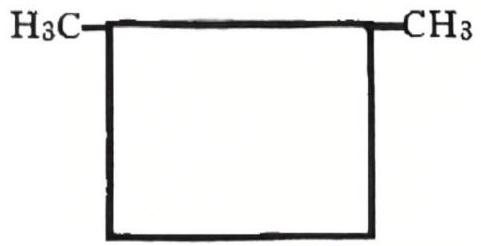
\includegraphics[max width=\textwidth, center]{2025_08_11_1fac7286a628a1b4eedag-39(6)}\\
A) 1.2 -dimetilsiklobutan\\
B) 1.3 -dimetilsiklobutan\\
C) siklobutan\\
D) 1.4-dimetilsiklobutan\\
  \item Quyidagi rasmda berilgan sikloalkanni sistematik nomenklaturada nomlang.\\
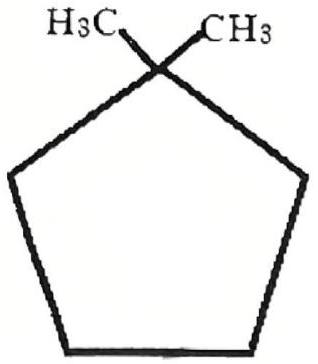
\includegraphics[max width=\textwidth, center]{2025_08_11_1fac7286a628a1b4eedag-40(1)}\\
A) 1.3-dimetilsiklopentan\\
B) 1.2-dimetilsiklopentan\\
C) 1.1-dimetilsiklopentan\\
D) 1.4 -dimetilsiklopentan
  \item Quyidagi rasmda berilgan sikloalkanni sistematik nomenklaturada nomlang.\\
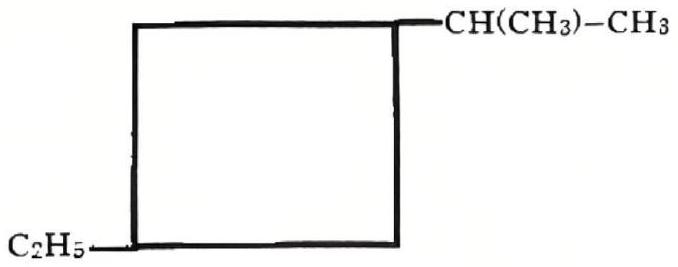
\includegraphics[max width=\textwidth, center]{2025_08_11_1fac7286a628a1b4eedag-40(4)}\\
A) 1-etil-4-izopropilsiklobutan\\
B) 1-etil-3-izopropilsiklobutan\\
C) 3-etil-1-izopropilsiklobutan\\
D) 2-etil-3-izopropilsiklobutan
  \item Quyidagi rasmda berilgan sikloalkanni sistematik nomenklaturada nomlang.\\
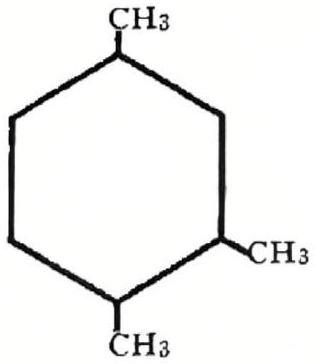
\includegraphics[max width=\textwidth, center]{2025_08_11_1fac7286a628a1b4eedag-40(3)}\\
A) 1.2.3-trimetilsiklogeksan\\
B) 1.2.5-trimetilsiklogeksan\\
C) 1.3.4-trimetilsiklogeksan\\
D) 1.2.4-trimetilsiklogeksan
  \item Quyidagi rasmda berilgan sikloalkanni sistematik nomenklaturada nomlang.\\
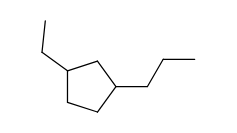
\includegraphics{smile-a9a5a947b19b8370168296fd8d4d28437b04c31d}\\
A) 1-propil-3-etilsiklobutan\\
B) 1-etil-3-propilsiklopentan\\
C) 1-etil-4-propilsiklobutan\\
D) 2-etil-3-propilsiklobutan
  \item Quyidagi rasmda berilgan sikloalkanni sistematik nomenklaturada nomlang.\\
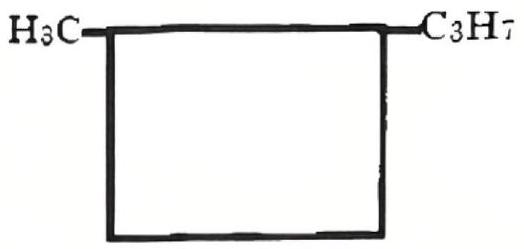
\includegraphics[max width=\textwidth, center]{2025_08_11_1fac7286a628a1b4eedag-40}\\
A) 1-metil-2-propilsiklobutan\\
B) 3-metil-3-propilsiklobutan\\
C) 1-propil-3-metilsiklobutan\\
D) 2 -metil- 3 -propilsiklobutan
  \item Quyidagi rasmda berilgan sikloalkanni sistematik nomenklaturada nomlang.\\
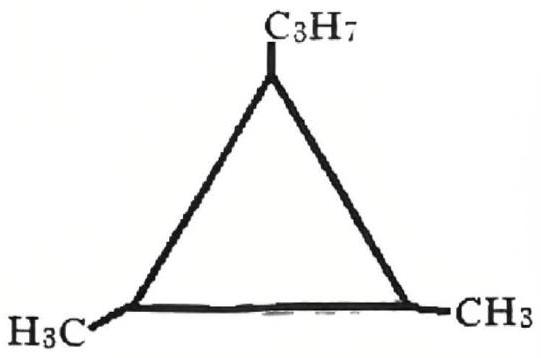
\includegraphics[max width=\textwidth, center]{2025_08_11_1fac7286a628a1b4eedag-40(2)}\\
A) 1.2-dimetil-2-propilsiklobutan\\
B) 1.2-dimetil-4-propilsiklobutan\\
C) 1.2-dimetil-3-propilsiklopropan\\
D) 1.2-dimetil-1-propilsiklobutan
  \item Quyidagi rasmda berilgan sikloalkanni sistematik nomenklaturada nomlang.\\
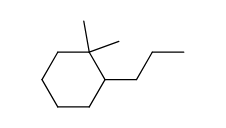
\includegraphics{smile-03cce9bc94dd5929e2007b24c5e925929151fce5}\\
A) 1.1-dimetil-3-propilsiklogeksan\\
B) 1.1 -dimetil-2-propilsiklogeksan\\
C) 1.1 -dimetil-4-propilsiklogeksan\\
D) 1.2 -dimetil-2-propilsiklogeksan
  \item Quyidagi rasmda berilgan sikloalkanni sistematik nomenklaturada nomlang.\\
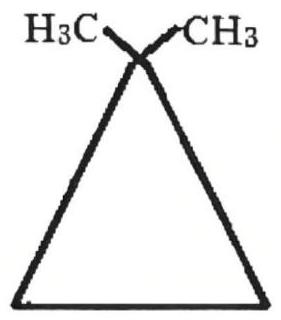
\includegraphics[max width=\textwidth, center]{2025_08_11_1fac7286a628a1b4eedag-41}\\
A) 1.1-dimetilsiklopropan\\
B) 1.2 -dimetilsiklopropan\\
C) 1.3-dimetilsiklopropan\\
D) 1-metilsiklopropan
  \item Quyidagi rasmda berilgan sikloalkanni sistematik nomenklaturada nomlang.\\
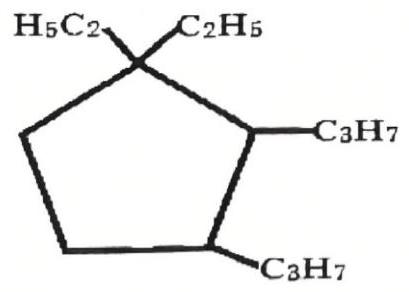
\includegraphics[max width=\textwidth, center]{2025_08_11_1fac7286a628a1b4eedag-41(2)}\\
A) 1.2-dietil-3.4-dipropilsiklopentan\\
B) 1.1 -dietil-3.3-dipropilsiklopentan\\
C) 1.1-dietil-3.4-dipropilsiklopentan\\
D) 1.4-dietil-3.4-dipropilsiklopentan
  \item 1.3-dibrompropanga Mg metali ta'sir ettirilganda qaysi sikloalkan hosil bo'ladi?\\
A) siklopropan\\
B) metilsiklopropan\\
C) 1.2 dimetilsiklobutan\\
D) 1.1-dimetilsiklobutan\\
  \item 1.2-dimetil-1.4-dixlorbutanga Zn metali ta'sir ettirilganda qaysi sikloalkan hosil bo'ladi?\\
A) siklopropan\\
B) metilsiklopropan\\
C) 1.2 -dimetilsiklobutan\\
D) 1.1-dimetilsiklobutan
  \item 1.3-dibrombutanga Mg metali ta'sir ettirilganda qaysi sikloalkan hosil bo'ladi?\\
A) siklopropan\\
B) metilsiklopropan\\
C) 1.2-dimetilsiklobutan\\
D) 1.1-dimetilsiklobutan
  \item 2.2-dimetil-1.4-dixlorbutanga Mg metali ta'sir ettirilganda qaysi sikloalkan hosil bo'ladi?\\
A) siklopropan\\
B) 2.2dimetilsiklopropan\\
C) 1.3 -dimetilsiklobutan\\
D) 1.1 -dimetilsiklobutan
  \item 2.4-dimetil-1.5-dixlorpentanga Mg metali ta'sir ettirilganda qaysi sikloalkan hosil bo'ladi?\\
A) propilsiklopropan\\
B) metilsiklopropan\\
C) 1.3-dimetilsiklopentan\\
D) 1.1-dimetilsiklobutan
  \item 1.3-dibromgeksanga Mg metali ta'sir ettirilganda qaysi sikloalkan hosil bo'ladi?\\
A) propilsiklopropan\\
B) metilsiklopropan\\
C) 1.3-dimetilsiklopentan\\
D) 1.1 -dimetilsiklobutan
  \item 2 -metil-3.5-dixlorpentanga Mg metali ta'sir ettirilganda qaysi sikloalkan hosil bo'ladi?\\
A) 1.3-dimetilsiklopropan\\
B) izopropilsiklopropan\\
C) 1.2 -dimetilsiklobutan\\
D) 1.4 -dimetilsiklobutan
  \item 1.6-dibromgeksanga Mg metali ta'sir ettirilganda qaysi sikloalkan hosil bo'ladi?\\
A) siklopropan\\
B) metilsiklopropan\\
C) metilsiklopentan\\
D) siklogeksan
  \item 1.3-dibrom-2-metilpropanga Mg metali ta'sir ettirilganda qaysi sikloalkan hosil bo'ladi?\\
A) siklopropan\\
B) metilsiklopropan\\
C) 1.2-dimetilsiklobutan\\
D) 1.1-dimetilsiklobutan
  \item 1.3-dibrompentanga Mg metali ta'sir ettirilganda qaysi sikloalkan hosil bo'ladi?\\
A) siklopropan\\
B) etilsiklopropan\\
C) 1.3 -dimetilsiklobutan\\
D) 1.2-dimetilsiklobutan
  \item $0,5 \mathrm{~mol}$ sikloalkanni to'la yondirish uchun da o'lchangan 252 litr havo sarflangan bo'lsa, sikloalkanni toping. (Havo tarkibida kislorodning hajmiy ulushi 20\%)\\
A) siklopropan\\
B) siklopentan\\
C) siklobutan\\
D) metilsiklopentan
  \item $1,5 \mathrm{~mol}$ sikloalkanni to'la yondirish uchun da o'lchangan 1512 litr havo sarflangan bo'lsa, sikloalkanni toping. (Havo tarkibida kislorodning hajmiy ulushi 20\%)\\
A) siklopropan\\
B) siklopentan\\
C) siklobutan\\
D) metilsiklopentan
  \item 1 mol sikloalkanni to'la yondirish uchun da o'lchangan 672 litr havo sarflangan bo'lsa, sikloalkanni toping. (Havo tarkibida kislorodning hajmiy ulushi 20\%)\\
A) siklopropan\\
B) siklopentan\\
C) siklobutan\\
D) metilsiklopentan
  \item $0,5 \mathrm{~mol}$ sikloalkanni to'la yondirish uchun da o'lchangan 420 litr havo sarflangan bo'lsa, sikloalkanni toping. (Havo tarkibida kislorodning hajmiy ulushi 20\%)\\
A) etilsiklopropan\\
B) etilsiklogeksan\\
C) propilsiklobutan\\
D) metilsiklopentan
  \item 2 mol sikloalkanni to'la yondirish uchun da o'lchangan 2352 litr havo sarflangan bo'lsa, sikloalkanni toping. (Havo tarkibida kislorodning hajmiy ulushi 20\%)\\
A) etilsiklopropan\\
B) etilsiklogeksan\\
C) propilsiklobutan\\
D) metilsiklopentan
  \item $0,2 \mathrm{~mol}$ sikloalkanni to'la yondirish uchun da o'lchangan 100,8 litr havo sarflangan bo'lsa, sikloalkanni toping. (Havo tarkibida kislorodning hajmiy ulushi 20\%)\\
A) siklopropan\\
B) siklopentan\\
C) siklobutan\\
D) metilsiklopentan
  \item $0,1 \mathrm{~mol}$ sikloalkanni to'la yondirish uchun da o'lchangan 100,8 litr havo sarflangan bo'lsa, sikloalkanni toping. (Havo tarkibida kislorodning hajmiy ulushi 20\%)\\
A) etilsiklopropan\\
B) etilsiklogeksan\\
C) propilsiklobutan\\
D) metilsiklopentan
  \item $0,4 \mathrm{~mol}$ sikloalkanni to'la yondirish uchun da o'lchangan 201,6 litr havo sarflangan bo'lsa, sikloalkanni toping. (Havo tarkibida kislorodning hajmiy ulushi 20\%)\\
A) siklopropan\\
B) siklopentan\\
C) siklobutan\\
D) metilsiklopentan
  \item $0,3 \mathrm{~mol}$ sikloalkanni to'la yondirish uchun da o'lchangan 252 litr havo sarflangan bo'lsa, sikloalkanni toping. (Havo tarkibida kislorodning hajmiy ulushi 20\%)\\
A) etilsiklopropan\\
B) etilsiklogeksan\\
C) propilsiklobutan\\
D) metilsiklopentan
  \item $0,8 \mathrm{~mol}$ sikloalkanni to'la yondirish uchun da o'lchangan 537,6 litr havo sarflangan bo'lsa, sikloalkanni toping.\\
(Havo tarkibida kislorodning hajmiy ulushi $20 \%$ )\\
A) siklopropan\\
B) siklopentan\\
C) siklobutan\\
D) metilsiklopentan
  \item Molekulasida 40 ta proton saqlagan sikloalkanni 35 g miqdoridan foydalanib necha g alkan olish mumkin?\\
A) 36\\
B) 40\\
C) 42\\
D) 44
  \item Molekulasida 24 ta proton saqlagan sikloalkanni 42 g miqdoridan foydalanib necha g alkan olish mumkin?\\
A) 36\\
B) 40\\
C) 42\\
D) 44
  \item Molekulasida 48 ta proton saqlagan sikloalkanni 168 g miqdoridan foydalanib necha g alkan olish mumkin?\\
A) 170\\
B) 172\\
C) 174\\
D) 176
  \item Molekulasida 32 ta proton saqlagan sikloalkanni $11,2 \mathrm{~g}$ miqdoridan foydalanib necha g alkan olish mumkin?\\
A) 12,4\\
B) 14\\
C) 11,6\\
D) 12,6
  \item Molekulasida 56 ta proton saqlagan sikloalkanni 49 g miqdoridan foydalanib necha g alkan olish mumkin?\\
A) 50\\
B) 53\\
C) 51\\
D) 52
  \item Molekulasida 40 proton saqlagan sikloalkanni 70 g miqdoridan foydalanib necha g alkan olish mumkin?\\
A) 76\\
B) 73\\
C) 72\\
D) 74
  \item Molekulasida 24 proton saqlagan sikloalkanni 21 g miqdoridan foydalanib necha g alkan olish mumkin?\\
A) 24\\
B) 22\\
C) 26\\
D) 23
  \item Molekulasida 32 proton saqlagan sikloalkanni 14 g miqdoridan foydalanib necha g alkan olish mumkin?\\
A) 15,5\\
B) 16\\
C) 15\\
D) 14,5
  \item Molekulasida 48 proton saqlagan sikloalkanni 42 g miqdoridan foydalanib necha g alkan olish mumkin?\\
A) 42\\
B) 45\\
C) 43\\
D) 44
  \item Siklopropan va siklobutandan iborat 49 g aralashma to'la gidrogenlanganda 51 g alkanlar aralashmasi olindi. Dastlabki aralashmadagi siklobutanni massasini (g) aniqlang.\\
A) 28\\
B) 21\\
C) 42\\
D) 24
  \item Siklopropan va siklobutandan iborat 49 g aralashma to'la gidrogenlanganda 51 g alkanlar aralashmasi olindi. Dastlabki aralashmadagi siklopropanni massasini (g) aniqlang.\\
A) 28\\
B) 21\\
C) 42\\
D) 24
  \item Siklopropan va siklobutandan iborat $33,6 \mathrm{~g}$ aralashma to'la gidrogenlanganda 35 g alkanlar aralashmasi olindi. Dastlabki aralashmadagi siklobutanni massasini (g) aniqlang.\\
A) 28\\
B) 22,4\\
C) 16,8\\
D) 5,6
  \item Siklopropan va siklobutandan iborat $25,2 \mathrm{~g}$ aralashma to'la gidrogenlanganda $26,2 \mathrm{~g}$ alkanlar aralashmasi olindi. Dastlabki aralashmadagi siklopropanni massasini ( g ) aniqlang.\\
A) 16,8\\
B) 8,4\\
C) 11,2\\
D) 5,6
  \item Siklopropan va siklobutandan iborat $39,2 \mathrm{~g}$ aralashma to'la gidrogenlanganda $40,8 \mathrm{~g}$ alkanlar aralashmasi olindi.\\
Dastlabki aralashmadagi siklobutanni massasini ( g ) aniqlang.\\
A) 28\\
B) 22,4\\
C) 16,8\\
D) 5,6
  \item Siklopropan va siklobutandan iborat $36,4 \mathrm{~g}$ aralashma to'la gidrogenlanganda 38 g alkanlar aralashmasi olindi. Dastlabki aralashmadagi siklobutanni massasini (g) aniqlang.\\
A) 16,8\\
B) 8,4\\
C) 11,2\\
D) 5,6
  \item Siklopropan va siklobutandan iborat $51,8 \mathrm{~g}$ aralashma to'la gidrogenlanganda 53.8 g alkanlar aralashmasi olindi. Dastlabki aralashmadagi siklopropanni massasini ( g ) aniqlang.\\
A) 12,6\\
B) 25,2\\
C) 14\\
D) 28
  \item Siklopropan va siklobutandan iborat $67,2 \mathrm{~g}$ aralashma to'la gidrogenlanganda 70 g alkanlar aralashmasi olindi. Dastlabki aralashmadagi siklobutanni massasini (g) aniqlang.\\
A) 28\\
B) 44,8\\
C) 33,6\\
D) 22,4
  \item Siklopropan va siklobutandan iborat $43,4 \mathrm{~g}$ aralashma to'la gidrogenlanganda $45,2 \mathrm{~g}$ alkanlar aralashmasi olindi. Dastlabki aralashmadagi siklopropanni massasini (g) aniqlang.\\
A) 28\\
B) 21\\
C) 42\\
D) 24
  \item Siklopropan va siklobutandan iborat $53,2 \mathrm{~g}$ aralashma to'la gidrogenlanganda $55,2 \mathrm{~g}$ alkanlar aralashmasi olindi. Dastlabki aralashmadagi siklobutanni massasini (g) aniqlang.\\
A) 28\\
B) 44,8\\
C) 33,6\\
D) 22,4
  \item Propan va siklopropandan iborat 64 g aralashma to'la gidrogenlanganda 66 g propan hosil bo'lsa, aralashma tarkibidagi siklopropan massasini (g) hisoblang.\\
A) 42\\
B) 21\\
C) 54\\
D) 27\\
  \item Propan va siklopropandan iborat 51,2 g aralashma to'la gidrogenlanganda $52,8 \mathrm{~g}$\\
propan hosil bo'lsa, aralashma tarkibidagi siklopropan massasini (g) hisoblang.\\
A) 22,4\\
B) 33,6\\
C) 44,8\\
D) 67,2
  \item Propan va siklopropandan iborat 21,4 g aralashma to'la gidrogenlanganda 22 g propan hosil bo'lsa, aralashma tarkibidagi propan massasini (g) hisoblang.\\
A) 17,6\\
B) 12,6\\
C) 4,4\\
D) 8,8
  \item Propan va siklopropandan iborat 38,6 g aralashma to'la gidrogenlanganda $39,6 \mathrm{~g}$ propan hosil bo'lsa, aralashma tarkibidagi propan massasini (g) hisoblang.\\
A) 22\\
B) 4,4\\
C) 17,6\\
D) 8,8
  \item Propan va siklopropandan iborat 17,2 g aralashma to'la gidrogenlanganda $17,6 \mathrm{~g}$ propan hosil bo'lsa, aralashma tarkibidagi siklopropan massasini (g) hisoblang.\\
A) 4,2\\
B) 8,4\\
C) 10,5\\
D) 16,8
  \item Butan va siklobutandan iborat $45,6 \mathrm{~g}$ aralashma to'la gidrogenlanganda 46.4 g butan hosil bo'lsa, aralashma tarkibidagi siklobutan massasini (g) hisoblang.\\
A) 5,6\\
B) 11,2\\
C) 22,4\\
D) 33,6
  \item Butan va siklobutandan iborat $28,6 \mathrm{~g}$ aralashma to'la gidrogenlanganda 29 g butan hosil bo'lsa, aralashma tarkibidagi siklobutan massasini (g) hisoblang.\\
A) 5,6\\
B) 11,2\\
C) 22,4\\
D) 33.6
  \item Butan va siklobutandan iborat $39,8 \mathrm{~g}$ aralashma to'la gidrogenlanganda $40,6 \mathrm{~g}$ butan hosil bo'lsa, aralashma tarkibidagi siklobutan massasini (g) hisoblang.\\
A) 5,6\\
B) 11,2\\
C) 22,4\\
D) 33,6
  \item Butan va siklobutandan iborat 57 g aralashma to'la gidrogenlanganda 58 g butan hosil bo'lsa, aralashma tarkibidagi butan massasini (g) hisoblang.\\
A) 29\\
B) 28\\
C) 27\\
D) 30
  \item Butan va siklobutandan iborat $68,8 \mathrm{~g}$ aralashma to'la gidrogenlanganda $69,6 \mathrm{~g}$ butan hosil bo'lsa, aralashma tarkibidagi butan massasini (g) hisoblang.\\
A) 23,2\\
B) 46,4\\
C) 29\\
D) 58
  \item 21 g siklopropan yonishidan hosil bo'lgan $\mathrm{CO}_{2}$ necha g KOH bilan reaksiyaga kirishadi? (Reaksiyadan faqat o'rta tuz hosil bo'lgan)\\
A) 168\\
B) 84\\
C) 56\\
D) 28
  \item 28 g siklobutan yonishidan hosil bo'lgan $\mathrm{CO}_{2}$ necha g KOH bilan reaksiyaga kirishadi? (Reaksiyadan faqat o'rta tuz hosil bo'lgan)\\
A) 168\\
B) 112\\
C) 224\\
D) 280
  \item 56 g metilsiklopropan yonishidan hosil bo'lgan $\mathrm{CO}_{2}$ necha g KOH bilan reaksiyaga kirishadi? (Reaksiyadan faqat o'rta tuz hosil bo'lgan)\\
A) 560\\
B) 448\\
C) 224\\
D) 336
  \item 35 g siklopentan yonishidan hosil bo'lgan $\mathrm{CO}_{2}$ necha g KOH bilan reaksiyaga kirishadi? (Reaksiyadan faqat o'rta tuz hosil bo'lgan)\\
A) 168\\
B) 184\\
C) 560\\
D) 280
  \item 42 g propilsiklopropan yonishidan hosil bo'lgan $\mathrm{CO}_{2}$ necha g KOH bilan reaksiyaga kirishadi? (Reaksiyadan faqat o'rta tuz hosil bo'lgan)\\
A) 560\\
B) 448\\
C) 224\\
D) 336
  \item 70 g metilsiklopropan yonishidan hosil bo'lgan $\mathrm{CO}_{2}$ necha g KOH bilan reaksiyaga kirishadi? (Reaksiyadan faqat o'rta tuz hosil bo'lgan)\\
A) 168\\
B) 184\\
C) 560\\
D) 280
  \item 84 g siklogeksan yonishidan hosil bo'lgan $\mathrm{CO}_{2}$ necha g KOH bilan reaksiyaga kirishadi? (Reaksiyadan faqat o'rta tuz hosil bo'lgan)\\
A) 672\\
B) 448\\
C) 224\\
D) 336
  \item 42 g siklopropan yonishidan hosil bo'lgan $\mathrm{CO}_{2}$ necha g KOH bilan reaksiyaga kirishadi? (Reaksiyadan faqat o'rta tuz hosil bo'lgan)\\
A) 672\\
B) 448\\
C) 224\\
D) 336
  \item 14 g etilsiklopropan yonishidan hosil bo'lgan $\mathrm{CO}_{2}$ necha g KOH bilan reaksiyaga kirishadi? (Reaksiyadan faqat o'rta tuz hosil bo'lgan)\\
A) 168\\
B) 112\\
C) 224\\
D) 280
  \item 56 g etilgeksan yonishidan hosil bo'lgan $\mathrm{CO}_{2}$ necha g KOH bilan reaksiyaga kirishadi? (Reaksiyadan faqat o'rta tuz hosil bo'lgan)\\
A) 672\\
B) 448\\
C) 224\\
D) 336
  \item Molekulasida 16 ta $\mathrm{sp}^{3}$ gibridlangan orbital saqlagan sikloalkanni toping, uning necha g miqdori $2 \mathrm{~mol} \mathrm{Cl}_{2}$ bilan birikish reaksiyasiga kirishadi?\\
A) siklopropan 42\\
B) siklobutan 112\\
C) metilsiklopentan 84\\
D) siklopentan 35
  \item Molekulasida 24 ta $\mathrm{sp}^{3}$ gibridlangan orbital saqlagan sikloalkanni toping, uning necha g miqdori $2 \mathrm{~mol} \mathrm{Cl}_{2}$ bilan birikish reaksiyasiga kirishadi?\\
A) siklopropan 84\\
B) siklobutan 56\\
C) metilsiklopentan 168\\
D) siklopentan 70
  \item Molekulasida 12 ta $\mathrm{sp}^{3}$ gibridlangan orbital saqlagan sikloalkanni toping, uning necha g miqdori $1 \mathrm{~mol} \mathrm{Cl}_{2}$ bilan birikish reaksiyasiga kirishadi?\\
A) siklopropan 42\\
B) siklobutan 112\\
C) metilsiklopentan 84\\
D) siklopentan 35
  \item Molekulasida 16 ta $\mathrm{sp}^{3}$ gibridlangan orbital saqlagan sikloalkanni toping, uning necha g miqdori $1,5 \mathrm{~mol} \mathrm{Cl}_{2}$ bilan birikish reaksiyasiga kirishadi?\\
A) siklopropan 84\\
B) siklogeksan 28\\
C) metilsiklopropan 84\\
D) siklopentan 70
  \item Molekulasida 20 ta $\mathrm{sp}^{3}$ gibridlangan orbital saqlagan sikloalkanni toping, uning necha g miqdori $1 \mathrm{~mol} \mathrm{Cl}_{2}$ bilan birikish reaksiyasiga kirishadi?\\
A) etilsiklopropan 70\\
B) siklobutan 56\\
C) metilsiklopentan 84\\
D) etilsiklopentan 35
  \item Molekulasida 24 ta spi gibridlangan orbital saqlagan sikloalkanni toping, uning necha g miqdori $1.5 \mathrm{~mol} \mathrm{Cl}_{2}$ bilan birikish reaksiyasiga kirishadi?\\
A) siklopropan 63\\
B) etilsiklobutan 126\\
C) metilsiklogegsan 84\\
D) siklopentan 140
  \item Molekulasida 28 ta $\mathrm{sp}^{3}$ gibridlangan orbital saqlagan sikloalkanni toping, uning necha g miqdori $0,5 \mathrm{~mol}, \mathrm{Cl}_{2}$ bilan birikish reaksiyasiga kirishadi?\\
A) etilsiklopropan 84\\
B) metilsiklobutan 49\\
C) propilsiklobutan 49\\
D) siklopentan 35
  \item Molekulasida 24 ta $\mathrm{sp}^{3}$ gibridlangan orbital saqlagan sikloalkanni toping, uning necha g miqdori $0,5 \mathrm{~mol} \mathrm{Cl}_{2}$ bilan birikish reaksiyasiga kirishadi?\\
A) siklopropan 42\\
B) siklobutan 56\\
C) metilsiklopentan 42\\
D) siklopentan 70
  \item Molekulasida 20 ta $\mathrm{sp}^{3}$ gibridlangan orbital saqlagan sikloalkanni toping, uning necha g miqdori $2,5 \mathrm{~mol} \mathrm{Cl}_{2}$ bilan birikish reaksiyasiga kirishadi?\\
A) metilsiklopropan 84\\
B) metilsiklobutan 175\\
C) metilsiklopentan 168\\
D) metilsiklogeksan 140
  \item Molekulasida 24 ta $\mathrm{sp}^{3}$ gibridlangan orbital saqlagan sikloalkanni toping, uning necha g miqdori $3 \mathrm{~mol} \mathrm{Cl}_{2}$ bilan birikish reaksiyasiga kirishadi?\\
A) izopropilsiklopropan 252\\
B) izopropilsiklobutan 252\\
C) etilsiklopentan 86\\
D) siklopentan 84
81. $0,5 \mathrm{~mol}$ sikloalkanni yondirish uchun 96 g ozon-kislorod aralashmasi sarflangan bo'lsa, sikloalkanni toping?\\
A) $\mathrm{C}_{4} \mathrm{H}_{8}$\\
B) $\mathrm{C}_{3} \mathrm{H}_{6}$\\
C) $\mathrm{C}_{5} \mathrm{H}_{10}$\\
D) $\mathrm{C}_{6} \mathrm{H}_{12}$
82. 1 mol sikloalkanni yondirish uchun 288 g ozon-kislorod aralashmasi sarflangan bo'lsa, sikloalkanni toping?\\
A) $\mathrm{C}_{4} \mathrm{H}_{8}$\\
B) $\mathrm{C}_{3} \mathrm{H}_{6}$\\
C) $\mathrm{C}_{5} \mathrm{H}_{10}$\\
D) $\mathrm{C}_{6} \mathrm{H}_{12}$\\
83. $1,5 \mathrm{~mol}$ sikloalkanni yondirish uchun 216 g ozon-kislorod aralashmasi sarflangan bo'lsa, sikloalkanni toping?\\
A) $\mathrm{C}_{1} \mathrm{H}_{8}$\\
B) $\mathrm{C}_{3} \mathrm{H}_{6}$\\
C) $\mathrm{C}_{5} \mathrm{H}_{10}$\\
D) $\mathrm{C}_{6} \mathrm{H}_{12}$\\
84. $1,5 \mathrm{~mol}$ sikloalkanni yondirish uchun 288 g ozon-kislorod aralashmasi sarflangan bo'lsa, sikloalkanni toping?\\
A) $\mathrm{C}_{4} \mathrm{H}_{8}$\\
B) $\mathrm{C}_{3} \mathrm{H}_{6}$\\
C) $\mathrm{C}_{5} \mathrm{H}_{10}$\\
D) $\mathrm{C}_{6} \mathrm{H}_{12}$\\
85. $0,5 \mathrm{~mol}$ sikloalkanni yondirish uchun 120 g ozon-kislorod aralashmasi sarflangan bo'lsa, sikloalkanni toping?\\
A) $\mathrm{C}_{4} \mathrm{H}_{8}$\\
B) $\mathrm{C}_{5} \mathrm{H}_{10}$\\
C) $\mathrm{C}_{7} \mathrm{H}_{14}$\\
D) $\mathrm{C}_{6} \mathrm{H}_{12}$\\
86. $0,1 \mathrm{~mol}$ sikloalkanni yondirish uchun $33,6 \mathrm{~g}$ ozon-kislorod aralashmasi sarflangan bo'lsa, sikloalkanni toping?\\
A) $\mathrm{C}_{4} \mathrm{H}_{8}$\\
B) $\mathrm{C}_{5} \mathrm{H}_{10}$\\
C) $\mathrm{C}_{7} \mathrm{H}_{14}$\\
D) $\mathrm{C}_{6} \mathrm{H}_{12}$\\
87. $0,2 \mathrm{~mol}$ sikloalkanni yondirish uchun $28,8 \mathrm{~g}$ ozon-kislorod aralashmasi sarflangan bo'lsa, sikloalkanni toping?\\
A) $\mathrm{C}_{4} \mathrm{H}_{8}$\\
B) $\mathrm{C}_{3} \mathrm{H}_{6}$\\
C) $\mathrm{C}_{5} \mathrm{H}_{10}$\\
D) $\mathrm{C}_{6} \mathrm{H}_{12}$\\
88. $0,3 \mathrm{~mol}$ sikloalkanni yondirish uchun 72 g ozon-kislorod aralashmasi sarflangan bo'lsa, sikloalkanni toping?\\
A) $\mathrm{C}_{4} \mathrm{H}_{8}$\\
B) $\mathrm{C}_{3} \mathrm{H}_{6}$\\
C) $\mathrm{C}_{5} \mathrm{H}_{10}$\\
D) $\mathrm{C}_{6} \mathrm{H}_{12}$\\
89. $0,8 \mathrm{~mol}$ sikloalkanni yondirish uchun $153,6 \mathrm{~g}$ ozon-kislorod aralashmasi sarflangan bo'lsa, sikloalkanni toping?\\
A) $\mathrm{C}_{4} \mathrm{H}_{8}$\\
B) $\mathrm{C}_{3} \mathrm{H}_{6}$\\
C) $\mathrm{C}_{5} \mathrm{H}_{10}$\\
D) $\mathrm{C}_{6} \mathrm{H}_{12}$\\
90. $0,1 \mathrm{~mol}$ sikloalkanni yondirish uchun $28,8 \mathrm{~g}$ ozon kislorod aralashmasi sarflangan bo'lsa, sikloalkanni toping?\\
A) $\mathrm{C}_{4} \mathrm{H}_{8}$\\
B) $\mathrm{C}_{3} \mathrm{H}_{6}$\\
C) $\mathrm{C}_{5} \mathrm{H}_{10}$\\
D) $\mathrm{C}_{6} \mathrm{H}_{12}$\\
91. 226 g dixloralkanga Mg metali ta'sir ettirilganda, $190 \mathrm{~g} \mathrm{MgCl}_{2}$ hosil bo'lsa, sikloalkanni toping.\\
A) $\mathrm{C}_{4} \mathrm{H}_{5}$\\
B) $\mathrm{C}_{3} \mathrm{H}_{6}$\\
C) $\mathrm{C}_{5} \mathrm{H}_{10}$\\
D) $\mathrm{C}_{6} \mathrm{H}_{12}$
  \item 155 g dixloralkanga Mg metali ta'sir ettirilganda. $95 \mathrm{~g} \mathrm{MgCl}_{2}$ hosil bo'lsa, sikloalkanni toping.\\
A) $\mathrm{C}_{4} \mathrm{H}_{5}$\\
B) $\mathrm{C}_{3} \mathrm{H}_{6}$\\
C) $\mathrm{C}_{5} \mathrm{H}_{10}$\\
D) $\mathrm{C}_{6} \mathrm{H}_{12}$
  \item 254 g dixloralkanga Mg metali ta'sir ettirilganda, $190 \mathrm{~g} \mathrm{MgCl}_{2}$ hosil bo'lsa, sikloalkanni toping.\\
A) $\mathrm{C}_{4} \mathrm{H}_{5}$\\
B) $\mathrm{C}_{3} \mathrm{H}_{6}$\\
C) $\mathrm{C}_{5} \mathrm{H}_{10}$\\
D) $\mathrm{C}_{6} \mathrm{H}_{12}$
  \item 56.5 g dixloralkanga Mg metali ta'sir ettirilganda, $47,5 \mathrm{~g} \mathrm{MgCl}_{2}$ hosil bo'lsa, sikloalkanni toping.\\
A) $\mathrm{C}_{4} \mathrm{H}_{5}$\\
B) $\mathrm{C}_{3} \mathrm{H}_{6}$\\
C) $\mathrm{C}_{5} \mathrm{H}_{10}$\\
D) $\mathrm{C}_{6} \mathrm{H}_{12}$
  \item 282 g dixloralkanga Mg metali ta'sir ettirilganda, $190 \mathrm{~g} \mathrm{MgCl}_{2}$ hosil bo'lsa, sikloalkanni toping.\\
A) $\mathrm{C}_{4} \mathrm{H}_{8}$\\
B) $\mathrm{C}_{3} \mathrm{H}_{6}$\\
C) $\mathrm{C}_{5} \mathrm{H}_{10}$\\
D) $\mathrm{C}_{6} \mathrm{H}_{12}$
  \item 310 g dixloralkanga Mg metali ta'sir ettirilganda, $190 \mathrm{~g} \mathrm{MgCl}_{2}$ hosil bo'lsa, sikloalkanni toping.\\
A) $\mathrm{C}_{4} \mathrm{H}_{8}$\\
B) $\mathrm{C}_{3} \mathrm{H}_{6}$\\
C) $\mathrm{C}_{5} \mathrm{H}_{10}$\\
D) $\mathrm{C}_{6} \mathrm{H}_{12}$
  \item 183 g dixloralkanga Mg metali ta'sir ettirilganda, $95 \mathrm{~g} \mathrm{MgCl}_{2}$ hosil bo'lsa, sikloalkanni toping.\\
A) $\mathrm{C}_{7} \mathrm{H}_{14}$\\
B) $\mathrm{C}_{5} \mathrm{H}_{10}$\\
C) $\mathrm{C}_{8} \mathrm{H}_{16}$\\
D) $\mathrm{C}_{6} \mathrm{H}_{12}$
  \item 564 g dixloralkanga Mg metali ta'sir ettirilganda, $380 \mathrm{~g} \mathrm{MgCl}_{2}$ hosil bo'lsa, sikloalkanni toping.\\
A) $\mathrm{C}_{7} \mathrm{H}_{14}$\\
B) $\mathrm{C}_{5} \mathrm{H}_{10}$\\
C) $\mathrm{C}_{8} \mathrm{H}_{16}$\\
D) $\mathrm{C}_{6} \mathrm{H}_{12}$
  \item 169 g dixloralkanga Mg metali ta'sir ettirilganda, $95 \mathrm{~g} \mathrm{MgCl}_{2}$ hosil bo'lsa, sikloalkanni toping.\\
A) $\mathrm{C}_{7} \mathrm{H}_{14}$\\
B) $\mathrm{C}_{5} \mathrm{H}_{10}$\\
C) $\mathrm{C}_{8} \mathrm{H}_{16}$\\
D) $\mathrm{C}_{6} \mathrm{H}_{12}$
  \item 127 g dixloralkanga Mg metali ta'sir ettirilganda, $95 \mathrm{~g} \mathrm{MgCl}_{2}$ hosil bo'lsa, sikloalkanni toping.\\
A) $\mathrm{C}_{4} \mathrm{H}_{8}$\\
B) $\mathrm{C}_{3} \mathrm{H}_{6}$\\
C) $\mathrm{C}_{5} \mathrm{H}_{10}$\\
D) $\mathrm{C}_{6} \mathrm{H}_{12}$
  \item Quyidagi alkenni ratsional nomenklatura bo'yicha nomlang.\\
$\mathrm{CH}_{2}=\mathrm{CH}-\mathrm{CH}_{3}$\\
A) metileten\\
B) dimetileten\\
C) 1 -metileten\\
D) propen
2. Quyidagi alkenni ratsional nomenklatura bo'yicha nomlang.\\
$\mathrm{CH}_{2}=\mathrm{CH}-\mathrm{CH}_{2}-\mathrm{CH}_{3}$\\
A) dimetileten\\
B) dietileten\\
C) etileten\\
D) buten-1\\
3. Quyidagi alkenni ratsional nomenklatura bo'yicha nomlang.\\
$\mathrm{CH}_{3}-\mathrm{CH}=\mathrm{C}-\mathrm{CH}_{3}$\\
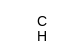
\includegraphics{smile-aeca3c740429068b3137485827915284fcd7e5fc}\\
A) dimetileten\\
B) trimetileten\\
C) 2-metilbuten-2\\
D) penten\\
4. Quyidagi alkenni ratsional nomenklatura bo'yicha nomlang.\\
$\mathrm{CH}_{3}-\mathrm{CH}=\mathrm{CH}-\mathrm{CH}-\mathrm{CH}_{3}$\\
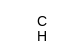
\includegraphics{smile-cb5f6e9e2c3630d16d8f572df3706b19916f223e}\\
A) trimetileten\\
B) 4-metilpenten-2\\
C) metil-propileten\\
D) metil-izopropileten\\
5. Quyidagi alkenni ratsional nomenklatura bo'yicha nomlang.\\
$\mathrm{CH}_{2}=\mathrm{CH}-\mathrm{CH}-\mathrm{CH}_{3}$\\
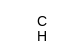
\includegraphics{smile-e050a21fe156978fa866065e229f13b0b224a2ca}\\
A) 3-metilbuten-1\\
B) dimetileten\\
C) trimetileten\\
D) izopropileten\\
8. Quyidagi alkenni ratsional nomenklatura bo'yicha nomlang.\\
$\mathrm{CH}_{3}-\mathrm{CH}_{2}-\mathrm{CH}=\mathrm{CH}-\mathrm{CH}_{3}$\\
A) metiletileten\\
B) dimetileten\\
C) metileten\\
D) penten-2\\
9. Quyidagi alkenni ratsional nomenklatura bo'yicha nomlang.\\
$\mathrm{CH}_{3}-\mathrm{C}=\mathrm{CH}-\mathrm{CH}_{2}-\mathrm{CH}_{3}$\\
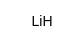
\includegraphics{smile-29d2b66b222f4c67ff47dfe19d333c0d4582ff78}\\
A) 4-metilgepten-3\\
B) dimetiletileten\\
C) metiletileten\\
D) metiletilpropileten\\
10. Quyidagi alkenni ratsional nomenklatura bo'yicha nomlang.\\
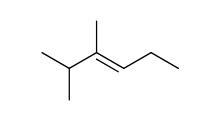
\includegraphics{smile-6f255e8b76173799ef22ae46ec5b21d06af9a753}\\
A) metiletileten\\
B) metiletilizopropileten\\
C) 2.3-dimetilgeksen-3\\
D) dimetiletileten
11. Quyidagi alkenni sistematik nomenklatura bo'yicha nomlang.\\
$\mathrm{CH}_{2}=\mathrm{CH}-\mathrm{CH}_{3}$\\
A) 1-metileten-1\\
B) 1.1 -dimetileten-1\\
C) 1-metileten-2\\
D) propen\\$\mathrm{CH}_{2}=\mathrm{CH}-\mathrm{CH}_{3}$\\
12. Quyidagi alkenni sistematik nomenklatura bo'yicha nomlang.\\
$\mathrm{CH}_{2}=\mathrm{CH}-\mathrm{CH}_{2}-\mathrm{CH}_{3}$\\
A) buten-1\\
B) buten-3\\
C) buten-2\\
D) buten-4\\
13. Quyidagi alkenni sistematik nomenklatura bo'yicha nomlang.\\
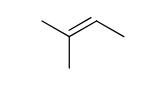
\includegraphics{smile-7a934ab3ee393367e795b3c50e4a5f9358382d59}\\
A) 3-metilbuten-2\\
B) 3-metilbuten-1\\
C) 2-metilbuten-2\\
D) penten\\
14. Quyidagi alkenni sistematik nomenklatura bo'yicha nomlang.\\
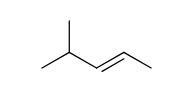
\includegraphics{smile-dafad08282609b7708f126c464532456b440294c}\\
A) 3-metilpenten-2 
B) 4 -metilpenten-2\\
C) 2 -metilpenten-2\\ 
D) 4 -metilpenten-1\\
15. Quyidagi alkenni sistematik nomenklatura bo'yicha nomlang.\\
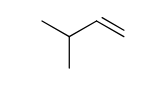
\includegraphics{smile-d4c833d58b867c5c3bf63391bc1fcb400ff887b6}\\
A) 3-metilbuten-1\\
B) 2 -metilbuten- 1\\
C) 2-metilbuten-2\\
D) 3 -metilbuten- 2\\
16. Quyidagi alkenni sistematik nomenklatura bo'yicha nomlang.\\
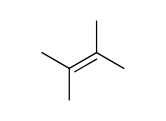
\includegraphics{smile-f3e62238eb6994e416f7e9284ae4f70721fd6afe}\\
A) 2.3 -dimetilbuten-2 
B) $2.4^{-}$ dimetilbuten-1\\
C) 2.4 -dimetilbuten-2 
D) 2.2 -dimetilbuten-2\\
17. Quyidagi alkenni sistematik nomenklatura bo'yicha nomlang.\\
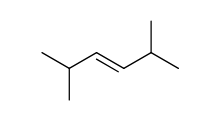
\includegraphics{smile-951b55e03cd339d5fe3deb892d3ac262f0e264a4}\\
A) 2.5 -dimetilgeksen- 1\\
B) 2.4 -dimetilgeksen- 2\\
C) 2.4 -dimetilgeksen- 3\\
D) 2.5 -dimetilgeksen-3\\
18. Quyidagi alkenni sistematik nomenklatura bo'yicha nomlang.\\
$\mathrm{CH}_{3}-\mathrm{CH}-\mathrm{CH}_{2}=\mathrm{CH}-\mathrm{CH}_{3}$\\
A) penten-2\\ 
B) penten-3\\
C) penten-1\\ 
D) penten-4\\
19. Quyidagi alkenni sistematik nomenklatura bo'yicha nomlang.\\
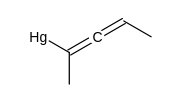
\includegraphics{smile-7fca49f24062868c39a1da6f8deab147e6208863}\\
A) 4-metilgepten-3\\
B) 2 -propilpenten- 2\\
C) 2 -propilpenten- 2\\
D) 4 -metilgepten- 2\\
20. Quyidagi alkenni sistematik nomenklatura bo'yicha nomlang.\\
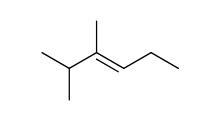
\includegraphics{smile-f063ef4bfcfd2d0ffed2258f3aafd1901288188f}\\
A) 2.3-dimetilgeksen-2\\
B) 2-izopropilpenten-2\\
C) 2.3 -dimetilgeksen-3\\
D) 2-izopropilpenten-1
  \item Molekulasida 18 ta neytron saqlagan alkenning necha g miqdori yonganda 66 g $\mathrm{CO}_{2}$ hosil bo'ladi?\\
A) 21\\ 
B) 42\\
C) 56\\
D) 112\\
  \item Molekulasida 24 ta neytron saqlagan alkenning necha g miqdori yonganda 88 g $\mathrm{CO}_{2}$ hosil bo'ladi?\\
A) 21\\
B) 28\\
C) 56\\
D) 11,2
  \item Molekulasida 30 ta neytron saqlagan alkenning necha g miqdori yonganda 220 g $\mathrm{CO}_{2}$ hosil bo'ladi?\\
A) 14\\
B) 35\\
C) 140\\
D) 70
  \item Molekulasida 36 ta neytron saqlagan alkenning necha g miqdori yonganda 132 g $\mathrm{CO}_{2}$ hosil bo'ladi?\\
A) 21\\
B) 42\\
C) 56\\
D) 112
  \item Molekulasida 42 ta neytron saqlagan alkenning necha g miqdori yonganda 154 g $\mathrm{CO}_{2}$ hosil bo'ladi?\\
A) 49\\
B) 98\\
C) 56\\
D) 112
  \item Molekulasida 30 ta neytron saqlagan alkenning necha g miqdori yonganda 44 g $\mathrm{CO}_{2}$ hosil boladi?\\
A) 7\\
B) 28\\
C) 14\\
D) 56
  \item Molekulasida 24 ta neytron saqlagan alkenning necha g miqdori yonganda 132 g $\mathrm{CO}_{2}$ hosil bo'ladi?\\
A) 21\\
B) 42\\
C) 56\\
D) 112
  \item Molekulasida 48 ta neytron saqlagan alkenning necha g miqdori yonganda 22 g $\mathrm{CO}_{2}$ hosil bo'ladi?\\
A) 7\\
B) 28\\
C) 14\\
D) 56
  \item Molekulasida 36 ta neytron saqlagan alkenning necha g miqdori yonganda 11 g $\mathrm{CO}_{2}$ hosil bo'ladi?\\
A) 7\\
B) 3,5\\
C) 14\\
D) 5,6
  \item Molekulasida 30 ta neytron saqlagan alkenning necha g miqdori yonganda 110 g $\mathrm{CO}_{2}$ hosil bo'ladi?\\
A) 14\\
B) 35\\
C) 140\\
D) 70
  \item Massasi 157 g bo'lgan $\mathrm{C}_{3} \mathrm{H}_{7} \mathrm{Cl}$ ga KOH ning spirtdagi eritmasini ta'sir ettirib necha g alken olish mumkin?\\
A) 84\\
B) 42\\
C) 56\\
D) 112
  \item Massasi $92,5 \mathrm{~g}$ bo'lgan $\mathrm{C}_{4} \mathrm{H}_{9} \mathrm{Cl}$ ga KOH ning spirtdagi eritmasini ta'sir ettirib necha g alken olish mumkin?\\
A) 84\\
B) 42\\
C) 56\\
D) 112
  \item Massasi 213 g bo'lgan $\mathrm{C}_{5} \mathrm{H}_{11} \mathrm{Cl}$ ga KOH ning spirtdagi eritmasini ta'sir ettirib necha g alken olish mumkin?\\
A) 140\\
B) 84\\
C) 56\\
D) 112
  \item Massasi 120.5 g bo'lgan $\mathrm{C}_{6} \mathrm{H}_{13} \mathrm{Cl}$ ga KOH ning spirtdagi eritmasini ta'sir ettirib necha g alken olish mumkin?\\
A) 84\\
B) 42\\
C) 56\\
D) 112
  \item Massasi $106,5 \mathrm{~g}$ bo'lgan $\mathrm{C}_{5} \mathrm{H}_{11} \mathrm{Cl}$ ga KOH ning spirtdagi eritmasini ta'sir ettirib necha g alken olish mumkin?\\
A) 84\\
B) 35\\
C) 56\\
D) 70
  \item Massasi $78,5 \mathrm{~g}$ bo'lgan $\mathrm{C}_{3} \mathrm{H}_{7} \mathrm{Cl}$ ga KOH ning spirtdagi eritmasini ta'sir ettirib necha g alken olish mumkin?\\
A) 84\\
B) 42\\
C) 56\\
D) 112
  \item Massasi 185 g bo'lgan $\mathrm{C}_{4} \mathrm{H}_{9} \mathrm{Cl}$ ga KOH ning spirtdagi eritmasini ta'sir ettirib necha $g$ alken olish mumkin?\\
A) 84\\
B) 42\\
C) 56\\
D) 112
  \item Massasi $134,5 \mathrm{~g}$ bo'lgan $\mathrm{C}_{7} \mathrm{H}_{15} \mathrm{Cl}$ ga KOH ning spirtdagi eritmasini ta'sir ettirib necha g alken olish mumkin?\\
A) 49\\
B) 98\\
C) 56\\
D) 112
  \item Massasi $21,3 \mathrm{~g}$ bo'lgan $\mathrm{C}_{5} \mathrm{H}_{13} \mathrm{Cl}$ ga KOH ning spirtdagi eritmasini ta'sir ettirib necha g alken olish mumkin?\\
A) 14\\
B) 2,8\\
C) 5,6\\
D) 11,2
  \item Massasi $18,5 \mathrm{~g}$ bo'lgan $\mathrm{C}_{4} \mathrm{H}_{9} \mathrm{Cl}$ ga KOH ning spirtdagi eritmasini ta'sir ettirib necha g alken olish mumkin?\\
A) 14\\
B) 2,8\\
C) 5,6\\
D) 11,2
  \item $16,8 \mathrm{~g}$ noma'lum alken $\mathrm{KMnO}_{4}$ ning suvli eritmasidan o'tkazilganda $0,2 \mathrm{~mol}$ cho'kma hosil boldi. Noma'lum alkenni toping.\\
A) $\mathrm{C}_{4} \mathrm{H}_{8}$\\
B) $\mathrm{C}_{3} \mathrm{H}_{6}$\\
C) $\mathrm{C}_{5} \mathrm{H}_{10}$\\
D) $\mathrm{C}_{6} \mathrm{H}_{12}$
  \item 42 g noma'lum alken $\mathrm{KMnO}_{4}$ ning suvli eritmasidan o'tkazilganda $0,4 \mathrm{~mol}$ cho'kma hosil boldi. Noma'lum alkenni toping.\\
A) $\mathrm{C}_{4} \mathrm{H}_{8}$\\
B) $\mathrm{C}_{3} \mathrm{H}_{6}$\\
C) $\mathrm{C}_{5} \mathrm{H}_{10}$\\
D) $\mathrm{C}_{6} \mathrm{H}_{12}$
  \item 12,6 g noma'lum alken $\mathrm{KMnO}_{4}$ ning suvli eritmasidan o'tkazilganda $0,2 \mathrm{~mol}$ cho'kma hosil boldi. Noma'lum alkenni toping.\\
A) $\mathrm{C}_{4} \mathrm{H}_{8}$\\
B) $\mathrm{C}_{3} \mathrm{H}_{6}$\\
C) $\mathrm{C}_{5} \mathrm{H}_{10}$\\
D) $\mathrm{C}_{6} \mathrm{H}_{12}$
  \item $8,4 \mathrm{~g}$ noma'lum alken $\mathrm{KMnO}_{4}$ ning suvli eritmasidan o'tkazilganda $0,1 \mathrm{~mol}$ cho'kma hosil boldi. Noma'lum alkenni toping.\\
A) $\mathrm{C}_{4} \mathrm{H}_{8}$\\
B) $\mathrm{C}_{3} \mathrm{H}_{6}$\\
C) $\mathrm{C}_{5} \mathrm{H}_{10}$\\
D) $\mathrm{C}_{6} \mathrm{H}_{12}$
  \item $50,4 \mathrm{~g}$ noma'lum alken $\mathrm{KMnO}_{4}$ ning suvli eritmasidan o'tkazilganda $0,4 \mathrm{~mol}$ cho'kma hosil boldi. Noma'lum alkenni toping.\\
A) $\mathrm{C}_{4} \mathrm{H}_{8}$\\
B) $\mathrm{C}_{3} \mathrm{H}_{6}$\\
C) $\mathrm{C}_{5} \mathrm{H}_{10}$\\
D) $\mathrm{C}_{6} \mathrm{H}_{12}$
  \item 21 g noma'lum alken $\mathrm{KMnO}_{4}$ ning suvli eritmasidan o'tkazilganda $0,2 \mathrm{~mol}$ cho'kma hosil boldi. Noma'lum alkenni toping.\\
A) $\mathrm{C}_{4} \mathrm{H}_{8}$\\
B) $\mathrm{C}_{3} \mathrm{H}_{6}$\\
C) $\mathrm{C}_{5} \mathrm{H}_{10}$\\
D) $\mathrm{C}_{6} \mathrm{H}_{12}$
  \item 42 g noma'lum alken $\mathrm{KMnO}_{4}$ ning suvli eritmasidan o'tkazilganda $0,5 \mathrm{~mol}$ cho'kma hosil boldi. Noma'lum alkenni toping.\\
A) $\mathrm{C}_{4} \mathrm{H}_{8}$\\
B) $\mathrm{C}_{3} \mathrm{H}_{6}$\\
C) $\mathrm{C}_{5} \mathrm{H}_{10}$\\
D) $\mathrm{C}_{6} \mathrm{H}_{12}$
  \item $25,2 \mathrm{~g}$ noma'lum alken $\mathrm{KMnO}_{4}$ ning suvli eritmasidan o'tkazilganda $0,4 \mathrm{~mol}$ cho'kma hosil boldi. Noma'lum alkenni toping.\\
A) $\mathrm{C}_{4} \mathrm{H}_{8}$\\
B) $\mathrm{C}_{3} \mathrm{H}_{6}$\\
C) $\mathrm{C}_{5} \mathrm{H}_{10}$\\
D) $\mathrm{C}_{6} \mathrm{H}_{12}$
  \item $52,5 \mathrm{~g}$ noma'lum alken $\mathrm{KMnO}_{4}$ ning suvli eritmasidan o'tkazilganda $0,5 \mathrm{~mol}$ cho'kma hosil boldi. Noma'lum alkenni toping.\\
A) $\mathrm{C}_{4} \mathrm{H}_{8}$\\
B) $\mathrm{C}_{3} \mathrm{H}_{6}$\\
C) $\mathrm{C}_{5} \mathrm{H}_{10}$\\
D) $\mathrm{C}_{6} \mathrm{H}_{12}$
  \item 84 g noma'lum alken $\mathrm{KMnO}_{4}$ ning suvli eritmasidan o'tkazilganda 1 mol cho'kma hosil boldi. Noma'lum alkenni toping.\\
A) $\mathrm{C}_{4} \mathrm{H}_{8}$\\
B) $\mathrm{C}_{3} \mathrm{H}_{6}$\\
C) $\mathrm{C}_{5} \mathrm{H}_{10}$\\
D) $\mathrm{C}_{6} \mathrm{H}_{12}$
  \item Butan va alkendan iborat $0,4 \mathrm{~mol}$ aralashma bromli suvdan o'tkazilganda idish massasi $8,4 \mathrm{~g}$ ga ortdi gazlarning\\
molekulalar soni esa 2 marta kamaydi. Alken molekulasidagi atomlar sonini aniqlang.\\
A) 9\\
B) 6\\
C) 12\\
D) 15
52. Propan va alkendan iborat $0,6 \mathrm{~mol}$ aralashma bromli suvdan o'tkazilganda idish massasi $5,6 \mathrm{~g}$ ga ortdi gazlarning molekulalar soni esa 1,5 marta kamaydi. Alken molekulasidagi atomlar sonini aniqlang.\\
A) 9\\
B) 6\\
C) 12\\
D) 15\\
53. Butan va alkendan iborat $0,5 \mathrm{~mol}$ aralashma bromli suvdan o'tkazilganda idish massasi 21 g ga ortdi gazlarning molekulalar soni esa 2,5 marta kamaydi. Alken molekulasidagi atomlar sonini aniqlang.\\
A) 9\\
B) 6\\
C) 12\\
D) 15\\
54. Butan va alkendan iborat $0,8 \mathrm{~mol}$ aralashma bromli suvdan o'tkazilganda idish massasi $16,8 \mathrm{~g}$ ga ortdi gazlarning molekulalar soni esa 4 marta kamaydi. Alken molekulasidagi atomlar sonini aniqlang.\\
A) 9\\
B) 6\\
C) 12\\
D) 15\\
55. Butan va alkendan iborat 1 mol aralashma bromli suvdan o'tkazilganda idish massasi $33,6 \mathrm{~g}$ ga ortdi gazlarning molekulalar soni esa 2,5 marta kamaydi. Alken molekulasidagi atomlar sonini aniqlang.\\
A) 9\\
B) 6\\
C) 12\\
D) 15\\
56. Butan va alkendan iborat $1,5 \mathrm{~mol}$ aralashma bromlí suvdan o'tkazilganda idish massasi 14 g ga ortdi gazlarning molekulalar soni esa 1,5 marta kamaydi. Alken molekulasidagi atomlar sonini aniqlang.\\
A) 9\\
B) 6\\
C) 12\\
D) 15\\
57. Butan va alkendan iborat $1,2 \mathrm{~mol}$ aralashma bromli suvdan o'tkazilganda idish massasi 70 g ga ortdi gazlarning molekulalar soni esa 6 marta kamaydi. Alken molekulasidagi atomlar sonini aniqlang.\\
A) 9\\
B) 6\\
C) 12\\
D) 15\\
58. Butan va alkendan iborat $0,6 \mathrm{~mol}$ aralashma bromli suvdan o'tkazilganda idish massasi $16,8 \mathrm{~g}$ ga ortdi gazlarning molekulalar soni esa 3 marta kamaydi. Alken molekulasidagi atomlar sonini aniqlang.\\
A) 9\\
B) 6\\
C) 12\\
D) 15\\
59. Butan va alkendan iborat $0,7 \mathrm{~mol}$ aralashma bromli suvdan o'tkazilganda idish massasi 14 g ga ortdi gazlarning molekulalar soni esa 3,5 marta kamaydi. Alken molekulasidagi atomlar sonini aniqlang.\\
A) 9\\
B) 6\\
C) 12\\
D) 15\\
60. Butan va alkendan iborat $0,75 \mathrm{~mol}$ aralashma bromli suvdan o'tkazilganda idish massasi 14 g ga ortdi gazlarning molekulalar soni esa 1,5 marta kamaydi. Alken molekulasidagi atomlar sonini aniqlang.\\
A) 9\\
B) 6\\
C) 12\\
D) 15
61. Massasi $14,7 \mathrm{~g}$ bo'lgan alken $5 \%$ li 480 g bromli suvni rangsizlantiradi. Alkenni toping.\\
A) buten\\
B) gepten\\
C) geksen\\
D) penten
  \item Massasi $11,2 \mathrm{~g}$ bo'lgan alken $2 \% \mathrm{li}$ 1600 g bromli suvni rangsizlantiradi. Alkenni toping.\\
A) buten\\
B) gepten\\
C) geksen\\
D) penten
  \item Massumi 7 o bo'lgan alken $4 \%$ li 400 g bromlj auvni rangsizlantiradi. Alkenni Loping.\\
A) buten\\
B) gepten\\
C) geksen\\
D) penten
  \item Massasi $8,4 \mathrm{~g}$ bo'lgan alken $5 \%$ lí 640 g bromli suvni rangsizlantíradi. Alkenni toping.\\
A) eten\\
B) propen\\
C) buten\\
D) penten
  \item Massasi 1.4 g bo'lgan alken $5 \%$ li 160 g bromli suvni rangsizlantiradi. Alkenni toping.\\
A) eten\\
B) propen\\
C) buten\\
D) penten
  \item Massasi $5,6 \mathrm{~g}$ bo'lgan alken $8 \%$ li 200 g bromli suvni rangsizlantiradi. Alkenni toping.\\
A) buten\\
B) gepten\\
C) geksen\\
D) penten
  \item Massasi $16,8 \mathrm{~g}$ bo'lgan alken $3,2 \%$ li 1000 g bromli suvni rangsizlantiradi. Alkenni toping.\\
A) buten\\
B) gepten\\
C) geksen\\
D) penten
  \item Massasi $29,4 \mathrm{~g}$ bo'lgan alken $10 \% \mathrm{li}$ 480 g bromli suvni rangsizlantiradi. Alkenni toping.\\
A) buten\\
B) gepten\\
C) geksen\\
D) penten
  \item Massasi $16,8 \mathrm{~g}$ bo'lgan alken $4,8 \% \mathrm{li}$ 1000 g bromli suvni rangsizlantiradi. Alkenni toping.\\
A) buten\\
B) gepten\\
C) geksen\\
D) penten
  \item Massasi 140 g bo'lgan alken $32 \%$ li 1000 g bromli suvni rangsizlantiradi. Alkenni toping.\\
A) buten\\
B) gepten\\
C) geksen\\
D) penten
71. Molekulasida 8 ta $\mathrm{sp}^{3}$ ta gibridlangan orbital saqlagan 112 g noma'lum alkenni\\
necha $g$ dixloralkandan sintez qilish mumkin?\\
A) 254\\
B) 127\\
C) 117\\
D) 234
72. Molekulasida 4 ta $\mathrm{sp}^{3}$ ta gibridlangan orbital saqlagan 42 g noma'lum alkenni necha g dixloralkandan sintez qilish mumkin?\\
A) 57\\
B) 114\\
C) 113\\
D) 226\\
73. Molekulasida 12 ta $\mathrm{sp}^{3}$ ta gibridlangan orbital saqlagan 140 g noma'lum alkenni necha g dixloralkandan sintez qilish mumkin?\\
A) 100,5\\
B) 211\\
C) 282\\
D) 140\\
74. Molekulasida 16 ta $\mathrm{sp}^{3}$ ta gibridlangan orbital saqlagan 168 g noma'lum alkenni necha g dixloralkandan sintez qilish mumkin?\\
A) 131\\
B) 262\\
C) 155\\
D) 310\\
75. Molekulasida 8 ta $\mathrm{sp}^{3}$ ta gibridlangan orbital saqlagan 56 g noma'lum alkenni necha g dixloralkandan sintez qilish mumkin?\\
A) 127\\
B) 114\\
C) 113\\
D) 226\\
76. Molekulasida 16 ta $\mathrm{sp}^{3}$ ta gibridlangan orbital saqlagan 84 g noma'lum alkenni necha g dixloralkandan sintez qilish mumkin?\\
A) 131\\
B) 262\\
C) 155\\
D) 310\\
77. Molekulasida 8 ta $\mathrm{sp}^{3}$ ta gibridlangan orbital saqlagan 14 g noma'lum alkenni necha g dixloralkandan sintez qilish mumkin?\\
A) 35,5\\
B) 63,5\\
C) 71\\
D) 31,75\\
78. Molekulasida 4 ta $\mathrm{sp}^{3}$ ta gibridlangan orbital saqlagan 21 g noma'lum alkenni necha g dixloralkandan sintez qilish mumkin?\\
A) 113\\
B) 35,4\\
C) 56,5\\
D) 23,4\\
79. Molekulasida 20 ta $\mathrm{sp}^{3}$ ta gibridlangan orbital saqlagan 49 g noma'lum alkenni necha g dixloralkandan sintez qilish mumkin?\\
A) 169\\
B) 84,5\\
C) 117\\
D) 234\\
80. Molekulasida 24 ta $\mathrm{sp}^{3}$ ta gibridlangan orbital saqlagan 112 g noma'lum alkenni necha g dixloralkandan sintez qilish mumkin?\\
A) 183\\
B) 255\\
C) 176\\
D) 211
  \item Labaratoriya sharoitida etilenni etil spirtidan olinadi. Necha g etil spirit parchalanganda hosil bo'lgan alken va suv massa farqi 20 g ga teng bo'ladi?\\
A) 92\\
B) 23\\
C) 46\\
D) 138
  \item Labaratoriya sharoitida etilenni etil spirtidan olinadi. Necha g etil spirit parchalanganda hosil bo'lgan alken va suv massa farqi 15 g ga teng bo'ladi?\\
A) 54\\
B) 27\\
C) 69\\
D) 138
  \item Labaratoriya sharoitida etilenni etil spirtidan olinadi. Necha g etil spirit parchalanganda hosil bo'lgan alken va suv massa farqi 30 g ga teng bo'ladi?\\
A) 92\\
B) 23\\
C) 46\\
D) 138
  \item Labaratoriya sharoitida etilenni etil spirtidan olinadi. Necha g etil spirit parchalanganda hosil bo'lgan alken va suv massa farqi 5 g ga teng bo'ladi?\\
A) 92\\
B) 23\\
C) 46\\
D) 138
  \item Labaratoriya sharoitida etilenni etil spirtidan olinadi. Necha g etil spirit parchalanganda hosil bo'lgan alken va suv massa farqi 45 g ga teng bo'ladi?\\
A) 105\\
B) 210\\
C) 103,5\\
D) 207
  \item Labaratoriya sharoitida etilenni etil spirtidan olinadi. Necha g etil spirit parchalanganda hosil bo'lgan alken va suv massa farqi 50 g ga teng bo'ladi?\\
A) 115\\
B) 92\\
C) 230\\
D) 460
  \item Labáratoriya sharoitida etilenni etil spirtidan olinadi. Necha g etil spirit parchalanganda hosil bo'lgan alken va suv massa farqi 8 g ga teng bo'ladi?\\
A) 36,8\\
B) 18,4\\
C) 73,6\\
D) 13,8
  \item Labaratoriya sharoitida etilenni etil spirtidan olinadi. Necha g etil spirit parchalanganda hosil bo'lgan alken va suv massa farqi 25 g ga teng bo'ladi?\\
A) 115\\
B) 92\\
C) 230\\
D) 460
  \item Labaratoriya sharoitida etilenni etil spirtidan olinadi. Necha g etil spirit parchalanganda hosil bo'lgan alken va suv massa farqi $2,5 \mathrm{~g}$ ga teng bo'ladi?\\
A) 9,2\\
B) 23\\
C) 11,5\\
D) 13,8
  \item Labaratoriya sharoitida etilenni etil spirtidan olinadi. Necha g etil spirit parchalanganda hosil bo'lgan alken va suv massa farqi 40 g ga teng bo'ladi?\\
A) 92\\
B) 184\\
C) 230\\
D) 138
  \item Quyidagi alkadiyenni sistematik nomenklaturada nomlang.\\
$\mathrm{CH}_{2}=\mathrm{CH}-\mathrm{CH}=\mathrm{CH}_{2}$\\
A) butadiyen-1.3\\
B) butadiyen- 1.4\\
C) butadiyen-1.1\\
D) butadiyen- 1.5\\
2. Quyidagi alkadiyenni sistematik nomenklaturada nomlang.\\
$\mathrm{CH}_{2}=\mathrm{C}\left(\mathrm{CH}_{3}\right)-\mathrm{CH}=\mathrm{CH}_{2}$\\
A) butadiyen- 1.3\\
B) 2 -metil butadiyen- 1.4\\
C) 2-metilbutadiyen-1.3\\
D) butadiyen-1.3\\
3. Quyidagi alkadiyenni sistematik nomenklaturada nomlang.\\
$\mathrm{CH}_{2}=\mathrm{C}\left(\mathrm{CH}_{3}\right)-\mathrm{C}\left(\mathrm{CH}_{3}\right)=\mathrm{CH}_{2}$\\
A) 2.2 -dimetibutadiyen- 1.2\\
B) 2.3-dimetibutadiyen- 1.4\\
C) 2.4-dimetibutadiyen-1.1\\
D) 2.3-dimetilbutadiyen-1.3\\
4. Quyidagi alkadiyenni sistematik nomenklaturada nomlang.\\
$\mathrm{CH}_{2}=\mathrm{C}\left(\mathrm{C}_{4} \mathrm{H}_{9}\right)-\mathrm{CH}=\mathrm{CH}-\mathrm{CH}_{3}$\\
A) 2-butilbutadiyen-1.3\\
B) 3-butilbutadiyen- 1.4\\
C) 2.3-dimetilbutadiyen-1.3\\
D) 2.4-dimetibutadiyen-1.1\\
5. Quyidagi alkadiyenni sistematik nomenklaturada nomlang.\\
$\mathrm{CH}_{2}=\mathrm{C}=\mathrm{CH}-\mathrm{CH}_{3}$\\
A) butadiyen-1.2\\
B) butadiyen-1.4\\
C) butadiyen-1.1\\
D) butadiyen-1.5\\
6. Quyidagi alkadiyenni sistematik nomenklaturada nomlang.\\
$\mathrm{CH}_{2}=\mathrm{CH}-\mathrm{CH}=\mathrm{CH}-\mathrm{CH}_{3}$\\
A) pentadiyen-1.2\\
B) pentadiyen-1.1\\
C) pentadiyen-1.3\\
D) pentadiyen-1.4\\
7. Quyidagi alkadiyenni sistematik nomenklaturada nomlang.\\
$\mathrm{CH}_{2}=\mathrm{C}\left(\mathrm{CH}_{3}\right)-\mathrm{C}\left(\mathrm{CH}_{3}\right)=\mathrm{CH}-\mathrm{CH}_{3}$\\
A) 2.3 -dimetilpentadiyen- 1.2\\
B) 2.3 -dimetilpentadiyen- 1.1\\
C) 2.3 -dimetilpentadiyen- 1.4\\
D) 2.3-dimetilpentadiyen-1.3\\
8. Quyidagi alkadiyenni sistematik nomenklaturada nomlang.\\
$\mathrm{CH}_{2}=\mathrm{C}=\mathrm{C}\left(\mathrm{CH}_{3}\right)-\mathrm{CH}_{2}$\\
A) 3 -metilbutadiyen- 1.2\\
B) 2-metilbutadiyen-1.2\\
C) 3-metilbutadiyen-1.3\\
D) 3-metilbutadiyen-1.4\\
9. Quyidagi alkadiyenni sistematik nomenklaturada nomlang.\\
$\mathrm{CH}_{2}=\mathrm{C}\left(\mathrm{C}_{2} \mathrm{H}_{5}\right)-\mathrm{CH}=\mathrm{CH}-\mathrm{CH}\left(\mathrm{CH}_{3}\right)-\mathrm{CH}_{3}$\\
A) 2 -etil- 5 -metilgeksadiyen-1.1\\
B) 2-etil-5-metilgeksadiyen-1.3\\
C) 2-etil-5-metilgeksadiyen-1.2\\
D) 2-etil-5-metilgeksadiyen-1.4\\
10. Quyídagi alkadiyenni sistematik nomenklaturada nomlang.\\
$\mathrm{CH}_{2}=\mathrm{CH}-\mathrm{CH}=\mathrm{CH}_{2}-\mathrm{CH}\left(\mathrm{CH}_{3}\right)-\mathrm{CH}_{3}$\\
A) 2 -metilgeksadiyen -1.3\\
B) 2-metilgeksadiyen-1.2\\
C) 5 -metilgeksadiyen- 1.2\\
D) 5 -metilgeksadiyen- 1.3
11. 46 g etil spirtidan foydalanib $80 \%$ unum bilan necha $g$ butadiyen- 1.3 olish mumkin?\\
A) 43,2\\
B) 54\\
C) 23\\
D) 21,6
  \item 92 g etil spirtidan foydalanib $90 \%$ unum bilan necha g butadiyen-1.3 olish mumkin?\\
A) 22,1\\
B) 48,6\\
C) 44,2\\
D) 24,3
  \item 23 g etil spirtidan foydalanib $60 \%$ unum bilan necha g butadiyen-1.3 olish mumkin?\\
A) 11,1\\
B) 22,2\\
C) 16,2\\
D) 8,1
  \item 92 g etil spirtidan foydalanib $50 \%$ unum bilan necha g butadiyen-1.3 olish mumkin?\\
A) 23\\
B) 54\\
C) 27\\
D) 46
  \item 69 g etil spirtidan foydalanib $40 \%$ unum bilan necha $g$ butadiyen- 1.3 olish mumkin?\\
A) 11,1\\
B) 22,2\\
C) 16,2\\
D) 8,1
  \item 46 g etil spirtidan foydalanib $75 \%$ unum bilan necha g butadiyen-1.3 olish mumkin?\\
A) 20,25\\
B) 40,5\\
C) 23,24\\
D) 46,48
  \item $9,2 \mathrm{~g}$ etil spirtidan foydalanib $80 \%$ unum bilan necha $g$ butadiyen- 1.3 olish mumkin?\\
A) 4,32\\
B) 5,4\\
C) 2,3\\
D) 4,46
  \item $4,6 \mathrm{~g}$ etil spirtidan foydalanib $70 \%$ unum bilan necha $g$ butadiyen- 1.3 olish mumkin?\\
A) 4,1\\
B) 1,89\\
C) 2,3\\
D) 0,9
  \item 69 g etil spirtidan foydalanib $50 \%$ unum bilan necha g butadiyen-1.3 olish mumkin?\\
A) 20,25\\
B) 40,5\\
C) 23,24\\
D) 46,48
  \item 92 g etil spirtidan foydalanib $100 \%$ unum bilan necha g butadiyen-1.3 olish mumkin?\\
A) 43,2\\
B) 54\\
C) 23\\
D) 44,6
  \item $1000 \mathrm{~g} 8 \%$ li bromli suvni rangsizlantirish uchun $12,1 \mathrm{~g}$ propadiyen va butadiyen aralashmasi sarflangan bo'lsa, aralashma tarkibidagi propadiyen massasini (g) aniqlang.\\
A) 4\\
B) 8\\
C) 2\\
D) 6\\
  \item $1000 \mathrm{~g} 25,6 \%$ li bromli suvni rangsizlantirish uchun $40,4 \mathrm{~g}$ propadiyen va butadiyen aralashmasi sarflangan bo'lsa, aralashma tarkibidagi propadiyen massasini (g) aniqlang.\\
A) 4\\
B) 8\\
C) 2\\
D) 6
  \item $1000 \mathrm{~g} 19,2 \%$ li bromli suvni rangsizlantirish uchun $29,6 \mathrm{~g}$ propadiyen va butadiyen aralashmasi sarflangan bo'lsa, aralashma tarkibidagi propadiyen massasini (g) aniqlang.\\
A) 4\\
B) 8\\
C) 2\\
D) 6
  \item $1000 \mathrm{~g} 19,2 \%$ li bromli suvni rangsizlantirish uchun 31 g propadiyen va butadiyen aralashmasi sarflangan bo'lsa, aralashma tarkibidagi propadiyen massasini (g) aniqlang.\\
A) 4\\
B) 8\\
C) 2\\
D) 6
  \item $1000 \mathrm{~g} 6,4 \%$ li bromli suvni rangsizlantirish uchun 10 g propadiyen va butadiyen aralashmasi sarflangan bo'lsa, aralashma tarkibidagi propadiyen massasini (g) aniqlang.\\
A) 4\\
B) 8\\
C) 2\\
D) 6
  \item $1000 \mathrm{~g} 3,2 \%$ li bromli suvni rangsizlantirish uchun $9,4 \mathrm{~g}$ propadiyen va butadiyen aralashmasi sarflangan\\
bo'lsa, aralashma tarkibidagi butadiyen massasini (g) aniqlang.\\
A) 5,4\\
B) 8,1\\
C) 10,8\\
D) 21,6
  \item $1000 \mathrm{~g} 19,2 \%$ li bromli suvni rangsizlantirish uchun $29,6 \mathrm{~g}$ propadiyen va butadiyen aralashmasi sarflangan bo'lsa, aralashma tarkibidagi butadiyen massasini (g) aniqlang.\\
A) 5,4\\
B) 8,1\\
C) 10,8\\
D) 21,6
  \item $1000 \mathrm{~g} 12,8 \%$ li bromli suvni rangsizlantirish uchun $36,2 \mathrm{~g}$ propadiyen va butadiyen aralashmasi sarflangan bo'lsa, aralashma tarkibidagi butadiyen massasini (g) aniqlang.\\
A) 5,4\\
B) 8,1\\
C) 10,8\\
D) 16,2
  \item $1000 \mathrm{~g} 9,6 \%$ li bromli suvni rangsizlantirish uchun $14,1 \mathrm{~g}$ propadiyen va butadiyen aralashmasi sarflangan bo'lsa, aralashma tarkibidagi butadiyen massasini (g) aniqlang.\\
A) 5,4\\
B) 8,1\\
C) 10,8\\
D) 21,6
  \item $1000 \mathrm{~g} 32 \%$ li bromli suvni rangsizlantirish uchun $49,4 \mathrm{~g}$ propadiyen va butadiyen aralashmasi sarflangan bo'lsa, aralashma tarkibidagi butadiyen massasini (g) aniqlang.\\
A) 5,4\\
B) 8,1\\
C) 10,8\\
D) 21,6
  \item $5,4 \mathrm{~g}$ butadiyen- 1.3 to'liq yonishidan hosil bo'lgan $\mathrm{CO}_{2}$ necha g $28 \%$ li KOH eritmasini to'la neytrallashga yetadi?\\
(Reaksiyada faqat o'rta tuz hosil bo'lgan)\\
A) 160\\
B) 200\\
C) 250\\
D) 300
  \item 27 g butadiyen- 1.3 to'liq yonishidan hosil bo'lgan $\mathrm{CO}_{2}$ necha $\mathrm{g} 14 \%$ li KOH eritmasini to'la neytrallashga yetadi? (Reaksiyada faqat o'rta tuz hosil bo'Igan)\\
A) 200\\
B) 400\\
C) 600\\
D) 1600
  \item $2,7 \mathrm{~g}$ butadiyen- 1.3 to'liq yonishidan hosil bo'lgan $\mathrm{CO}_{2}$ necha g 56 \% li KOH eritmasini to'la neytrallashga yetadi?\\
(Reaksiyada faqat o'rta tuz hosil bo'lgan)\\
A) 20\\
B) 40\\
C) 28\\
D) 56
  \item 4 g propadiyen to'liq yonishidan hosil bo'lgan $\mathrm{CO}_{2}$ necha g $28 \%$ li KOH eritmasini to'la neytrallashga yetadi?\\
(Reaksiyada faqat o'rta tuz hosil bo'lgan)\\
A) 120\\
B) 200\\
C) 240\\
D) 400
  \item 20 g propadiyen to'liq yonishidan hosil bo'lgan $\mathrm{CO}_{2}$ necha g $56 \%$ li KOH eritmasini to'la neytrallashga yetadi?\\
(Reaksiyada faqat o'rta tuz hosil bo'lgan)\\
A) 160\\
B) 200\\
C) 250\\
D) 300
  \item 8 g propadiyen to'liq yonishidan hosil bo'lgan $\mathrm{CO}_{2}$ necha g $28 \%$ li KOH eritmasini to'la neytrallashga yetadi? (Reaksiyada faqat o'rta tuz hosil bo'lgan)\\
A) 120\\
B) 200\\
C) 240\\
D) 400
  \item $3,4 \mathrm{~g}$ pentadiyen ${ }^{-1.3}$ to'liq yonishidan hosil bo'lgan $\mathrm{CO}_{2}$ necha g $2,8 \%$ li KOH eritmasini to'la neytrallashga yetadi? (Reaksiyada faqat o'rta tuz hosil bo'lgan)\\
A) 560\\
B) 600\\
C) 800\\
D) 1000
  \item $6,8 \mathrm{~g}$ pentadiyen- 1.3 to'liq yonishidan hosil bo'lgan $\mathrm{CO}_{2}$ necha g $56 \%$ li KOH eritmasini to'la neytrallashga yetadi? (Reaksiyada faqat o'rta tuz hosil bo'lgan)\\
A) 160\\
B) 100\\
C) 80\\
D) 200
  \item $13,6 \mathrm{~g}$ pentadiyen $\cdot 1.3$ to'liq yonishidan hosil bo'lgan $\mathrm{CO}_{2}$ necha $\mathrm{g} 56 \%$ li KOH eritmasini to'la neytrallashga yetadi? (Reaksiyada faqat o'rta tuz hosil bo'lgan)\\
A) 160\\
B) 200\\
C) 250\\
D) 300
  \item $4,1 \mathrm{~g}$ geksadiyen-1.3 to'liq yonishidan hosil bo'lgan $\mathrm{CO}_{2}$ necha g $56 \%$ li KOH eritmasini to'la neytrallashga yetadi? (Reaksiyada faqat o'rta tuz hosil bo'lgan)\\
A) 60\\
B) 30\\
C) 120\\
D) 90
  \item Butandan yuqori tempiratura va katalizator ishtirokida 54 g butadiyen\\
olindi. Reaksiya natijasida hosil bo'lgan vodorod bilan necha g propadiyenni to'la gidrogenlash mumkin?\\
A) 40\\
B) 30\\
C) 60\\
D) 90
  \item Butandan yuqori tempiratura va katalizator ishtirokida 27 g butadiyen olindi. Reaksiya natijasida hosil bo'lgan vodorod bilan necha g propadiyenni to'la gidrogenlash mumkin?\\
A) 25\\
B) 30\\
C) 20\\
D) 80
  \item Butandan yuqori tempiratura va katalizator ishtirokida 108 g butadiyen olindi. Reaksiya natijasida hosil bo'lgan vodorod bilan necha g propadiyenni to'la gidrogenlash mumkin?\\
A) 120\\
B) 30\\
C) 60\\
D) 80
  \item Butandan yuqori tempiratura va katalizator ishtirokida $5,4 \mathrm{~g}$ butadiyen olindi. Reaksiya natijasida hosil bo'lgan vodorod bilan necha g propadiyenni to'la gidrogenlash mumkin?\\
A) 4\\
B) 2\\
C) 6\\
D) 8
  \item Butandan yuqori tempiratura va katalizator ishtirokida $13,5 \mathrm{~g}$ butadiyen olindi. Reaksiya natijasida hosil bo'lgan vodorod bilan necha g propadiyenni to'la gidrogenlash mumkin?\\
A) 6\\
B) 8\\
C) 15\\
D) 10
  \item Butandan yuqori tempiratura va katalizator ishtirokida $10,8 \mathrm{~g}$ butadiyen olindi. Reaksiya natijasida hosil bo'lgan vodorod bilan necha g propadiyenni to'la gidrogenlash mumkin?\\
A) 6\\
B) 8\\
C) 15\\
D) 10
  \item Butandan yuqori tempiratura va katalizator ishtirokida $21,6 \mathrm{~g}$ butadiyen olindi. Reaksiya natijasida hosil bo'lgan vodorod bilan necha g propadiyenni to'la gidrogenlash mumkin?\\
A) 16\\
B) 32\\
C) 24\\
D) 40
  \item Butandan yuqori tempiratura va katalizator ishtirokida 43.2 g butadiyen olindi. Reaksiya natijasida hosil bo'lgan vodorod bilan necha g propadiyenni to'la gidrogenlash mumkin?\\
A) 16\\
B) 32\\
C) 24\\
D) 40
  \item Butandan yuqori tempiratura va katalizator ishtirokida 32.4 g butadiyen olindi. Reaksiya natijasida hosil bo'lgan vodorod bilan necha g propadiyenni to'la gidrogenlash mumkin?\\
A) 16\\
B) 32\\
C) 24\\
D) 40
  \item Butandan yuqori tempiratura va katalizator ishtirokida 270 g butadiyen olindi. Reaksiya natijasida hosil bo'lgan vodorod bilan necha g propadiyenni to'la gidrogenlash mumkin?\\
A) 200\\
B) 300\\
C) 400\\
D) 240
51. 17 g noma'lum alkadiyenni to'liq yondirilganda $55 \mathrm{~g} \mathrm{CO}_{2}$ hosil bo'ldi. Noma'lum alkadiyenni toping.\\
A) butadiyen-1.3\\
B) pentadiyen-1.2\\
C) propadiyen\\
D) geksadiyen-1.3
  \item 20 g noma'lum alkadiyenni to'liq yondirilganda $66 \mathrm{~g} \mathrm{CO}_{2}$ hosil bo'ldi. Noma'lum alkadiyenni toping.\\
A) butadiyen-1.3\\
B) pentadiyen-1.2\\
C) propadiyen\\
D) geksadiyen-1.3
  \item $6,8 \mathrm{~g}$ noma'lum alkadiyenni to'liq yondirilganda $22 \mathrm{~g} \mathrm{CO}_{2}$ hosil bo'ldi. Noma'lum alkadiyenni toping.\\
A) butadiyen-1.3\\
B) pentadiyen-1.2\\
C) propadiyen\\
D) geksadiyen-1.3
  \item 41 g noma'lum alkadiyenni to'liq yondirilganda $132 \mathrm{~g} \mathrm{CO}_{2}$ hosil bo'ldi. Noma'lum alkadiyenni toping.\\
A) butadiyen-1.3\\
B) pentadiyen-1.2\\
C) propadiyen\\
D) geksadiyen-1.3
  \item 10 g noma'lum alkadiyenni to'liq yondirilganda $33 \mathrm{~g} \mathrm{CO}_{2}$ hosil bo'ldi. Noma'lum alkadiyenni toping.\\
A) butadiyen-1.3\\
B) pentadiyen-1.2\\
C) propadiyen\\
D) geksadiyen-1.3
  \item $21,6 \mathrm{~g}$ noma'lum alkadiyenni to'liq yondirilganda $70,4 \mathrm{~g} \mathrm{CO}_{2}$ hosil bo'ldi. Noma'lum alkadiyenni toping.\\
A) butadiyen-1.3\\
B) pentadiyen-1.2\\
C) propadiyen\\
D) geksadiyen-1.3
  \item 34 g noma'lum alkadiyenni to'liq yondirilganda $110 \mathrm{~g} \mathrm{CO}_{2}$ hosil bo'ldi. Noma'lum alkadiyenni toping.\\
A) butadiyen-1.3\\
B) pentadiyen-1.2\\
C) propadiyen\\
D) geksadiyen-1.3
  \item 8 g noma'lum alkadiyenni to'liq yondirilganda $26,4 \mathrm{~g} \mathrm{CO}_{2}$ hosil bo'ldi. Noma'lum alkadiyenni toping.\\
A) butadiyen-1.3\\
B) pentadiyen-1.2\\
C) propadiyen\\
D) geksadiyen-1.3
  \item $8,2 \mathrm{~g}$ noma'lum alkadiyenni to'liq yondirilganda $26,4 \mathrm{~g} \mathrm{CO}_{2}$ hosil bo'ldi. Noma'lum alkadiyenni toping.\\
A) butadiyen-1.3\\
B) pentadiyen-1.2\\
C) propadiyen\\
D) geksadiyen-1.3
  \item 40 g noma'lum alkadiyenni to'liq yondirilganda $132 \mathrm{~g} \mathrm{CO}_{2}$ hosil bo'ldi. Noma'lum alkadiyenni toping.\\
A) butadiyen-1.3\\
B) pentadiyen-1.2\\
C) propadiyen\\
D) geksadiyen-1.3
  \item Etan va noma'lum alkadiyendan iborat 55 g aralashma bromli suv solingan idishdan o'tkazilganda idish massasi 40 g ga ortdi. Huddi shunday aralashma to'liq yondirilganda $176 \mathrm{~g} \mathrm{CO}_{2}$ hosil bo'lsa, noma'lum alkadiyenni toping.\\
A) butadiyen-1.3\\
B) pentadiyen-1.2\\
C) propadiyen\\
D) geksadiyen-1.3
  \item Metan va noma'lum alkadiyendan iborat 43 g aralashma bromli suv solingan idishdan o'tkazilganda idish massasi 27 g ga ortdi. Huddi shunday aralashma to'liq yondirilganda $132 \mathrm{~g} \mathrm{CO}_{2}$ hosil bo'lsa, noma'lum alkadiyenni toping.\\
A) butadiyen-1.3\\
B) pentadiyen-1.2\\
C) propadiyen\\
D) geksadiyen-1.3
  \item Propan va noma'lum alkadiyendan iborat 56 g aralashma bromli suv solingan idishdan o'tkazilganda idish massasi 34 g ga ortdi. Huddi shunday aralashma to'liq yondirilganda $176 \mathrm{~g} \mathrm{CO}_{2}$ hosil bo'lsa, noma'lum alkadiyenni toping.\\
A) butadiyen- 1.3\\
B) pentadiyen-1.2\\
C) propadiyen\\
D) geksadiyen-1.3
  \item Etan va noma'lum alkadiyendan iborat $27,6 \mathrm{~g}$ aralashma bromli suv solingan idishdan o'tkazilganda idish massasi 21,6 g ga ortdi. Huddi shunday aralashma to'liq yondirilganda $88 \mathrm{~g} \mathrm{CO}_{2}$ hosil bo'lsa, noma'lum alkadiyenni toping.\\
A) butadiyen- 1.3\\
B) pentadiyen-1.2\\
C) propadiyen\\
D) geksadiyen-1.3
  \item Butan va noma'lum alkadiyendan iborat 45 g aralashma bromli suv solingan idishdan o'tkazilganda idish massasi 16 g ga ortdi. Huddi shunday aralashma to'liq yondirilganda $140,8 \mathrm{~g} \mathrm{CO}_{2}$ hosil bo'lsa, noma'lum alkadiyenni toping.\\
A) butadiyen-1.3\\
B) pentadiyen-1.2\\
C) propadiyen\\
D) geksadiyen-1.3
  \item Metan va noma'lum alkadiyendan iborat 7 g aralashma bromli suv solingan idishdan o'tkazilganda idish massasi $5,4 \mathrm{~g}$ ga ortdi. Huddi shunday aralashma to'liq\\
yondirilganda $22 \mathrm{~g} \mathrm{CO}_{2}$ hosil bo'lsa, noma'lum alkadiyenni toping.\\
A) butadiyen- 1.3\\
B) pentadiyen-1.2\\
C) propadiyen\\
D) geksadiyen-1.3
  \item Propan va noma'lum alkadiyendan iborat $16,8 \mathrm{~g}$ aralashma bromli suv solingan idishdan o'tkazilganda idish massasi 8 g ga ortdi. Huddi shunday aralashma to'liq yondirilganda $52,8 \mathrm{~g} \mathrm{CO}_{2}$ hosil bo'lsa, noma'lum alkadiyenni toping.\\
A) butadiyen- 1.3\\
B) pentadiyen-1.2\\
C) propadiyen\\
D) geksadiyen-1.3
  \item Metan va noma'lum alkadiyendan iborat $9,8 \mathrm{~g}$ aralashma bromli suv solingan idishdan o'tkazilganda idish massasi $8,2 \mathrm{~g}$ ga ortdi. Huddi shunday aralashma to'liq yondirilganda $30,8 \mathrm{~g} \mathrm{CO}_{2}$ hosil bo'lsa, noma'lum alkadiyenni toping.\\
A) butadiyen- 1.3\\
B) pentadiyen-1.2\\
C) propadiyen\\
D) geksadiyen-1.3
  \item Etan va noma'lum alkadiyendan iborat 55 g aralashma bromli suv solingan idishdan o'tkazilganda idish massasi 40 g ga ortdi. Huddi shunday aralashma to'liq yondirilganda $176 \mathrm{~g} \mathrm{CO}_{2}$ hosil bo'lsa, noma'lum alkadiyenni toping.\\
A) butadiyen- 1.3\\
B) pentadiyen-1.2\\
C) propadiyen\\
D) geksadiyen-1.3
  \item Propan va noma'lum alkadiyendan iborat $9,8 \mathrm{~g}$ aralashma bromli suv solingan idishdan o'tkazilganda idish massasi $5,4 \mathrm{~g}$ ga ortdi. Huddi shunday aralashma to'liq yondirilganda $30,8 \mathrm{~g} \mathrm{CO}_{2}$ hosil bo'lsa, noma'lum alkadiyenni toping.\\
A) butadiyen- 1.3\\
B) pentadiyen-1.2\\
C) propadiyen\\
D) geksadiyen-1.3
  \item $\mathrm{C}_{20} \mathrm{H}_{38}$ tarkibli alkadiyen molekulasida 2 ta sp gibridlangan orbital bo'lsa, molekula tarkibidagi $\mathrm{sp}^{3}$ gibridlangan orbitallar sonini aniqlang.\\
A) 68\\
B) 56\\
C) 16\\
D) 44
72. $\mathrm{C}_{32} \mathrm{H}_{60}$ tarkibli alkadiyen molekulasida 12 ta $\mathrm{sp}^{2}$ gibridlangan orbital bo'lsa, molekula tarkibidagi sp ${ }^{3}$ gibridlangan orbitallar sonini aniqlang.\\
A) 118\\
B) 110\\
C) 116\\
D) 112\\
73. $\mathrm{C}_{25} \mathrm{H}_{48}$ tarkibli alkadiyen molekulasida 2 ta sp gibridlangan orbital bo'lsa, molekula tarkibidagi $\mathrm{sp}^{3}$ gibridlangan orbitallar sonini aniqlang.\\
A) 84\\
B) 88\\
C) 16\\
D) 44\\
74. $\mathrm{C}_{33} \mathrm{H}_{64}$ tarkibli alkadiyen molekulasida 12 ta $\mathrm{sp}^{2}$ gibridlangan orbital bo'lsa, molekula tarkibidagi sp ${ }^{3}$ gibridlangan orbitallar sonini aniqlang.\\
A) 118\\
B) 110\\
C) 116\\
C) 112\\
75. $\mathrm{C}_{22} \mathrm{H}_{42}$ tarkibli alkadiyen molekulasida 2 ta sp gibridlangan orbital bo'lsa, molekula tarkibidagi sp ${ }^{3}$ gibridlangan orbitallar sonini aniqlang.\\
A) 76\\
B) 80\\
C) 78\\
D) 84\\
76. $\mathrm{C}_{15} \mathrm{H}_{28}$ tarkibli alkadiyen molekulasida 12 ta $\mathrm{sp}^{2}$ gibridlangan orbital bo'lsa, molekula tarkibidagi $\mathrm{sp}^{3}$ gibridlangan orbitallar sonini aniqlang.\\
A) 68\\
B) 56\\
C) 16\\
D) 44\\
77. $\mathrm{C}_{50} \mathrm{H}_{98}$ tarkibli alkadiyen molekulasida 2 ta sp gibridlangan orbital bo'lsa, molekula tarkibidagi sp ${ }^{3}$ gibridlangan orbitallar sonini aniqlang.\\
A) 168\\
B) 156\\
C) 188\\
D) 176\\
78. $\mathrm{C}_{12} \mathrm{H}_{22}$ tarkibli alkadiyen molekulasida 12 ta sp² gibridlangan orbital bo'lsa, molekula tarkibidagi sp ${ }^{3}$ gibridlangan orbitallar sonini aniqlang.\\
A) 36\\
B) 32\\
C) 28\\
D) 40\\
79. $\mathrm{C}_{27} \mathrm{H}_{52}$ tarkibli alkadiyen molekulasida 2 ta sp gibridlangan orbital bo'lsa, molekula tarkibidagi sp ${ }^{3}$ gibridlangan orbitallar sonini aniqlang.\\
A) 96\\
B) 92\\
C) 88\\
D) 84\\
80. $\mathrm{C}_{14} \mathrm{H}_{26}$ tarkibli alkadiyen molekulasida 12 ta $\mathrm{sp}^{2}$ gibridlangan orbital bo'lsa, molekula tarkibidagi $\mathbf{s p}^{3}$ gibridlangan orbitallar sonini aniqlang.\\
A) 36\\
B) 34\\
C) 38\\
D) 40
  \item Molekulasi tarkibidagi protonlaridan neytronlari soni ayirmasi 4 ga teng bo'lgan alkadiyenning necha g miqdorini to'liq yonishidan hosil bo'lgan karbonat angidirid $500 \mathrm{~g} 48 \%$ li NaOH eritmasini to'liq neytrallaydi? (Reaksiyada faqat o'rta tuz hosil bo'lgan)\\
A) 36\\
B) 34\\
C) 38\\
D) 40
  \item Molekulasi tarkibidagi protonlaridan neytronlari soni ayirmasi 6 ga teng bo'lgan alkadiyenning necha g miqdorini to'liq yonishidan hosil bo'lgan karbonat angidirid $500 \mathrm{~g} 44,8 \%$ li KOH eritmasini to'liq neytrallaydi? (Reaksiyada faqat o'rta tuz hosil bo'lgan)\\
A) 27\\
B) 54\\
C) 10,8\\
D) 108
  \item Molekulasi tarkibidagi protonlaridan neytronlari soni ayirmasi 6 ga teng bo'lgan alkadiyenning necha g miqdorini to'liq yonishidan hosil bo'lgan karbonat angidirid $500 \mathrm{~g} 64 \%$ li NaOH eritmasini to'liq neytrallaydi?\\
A) 27\\
B) 54\\
C) 10,8\\
D) 108
  \item Molekulasi tarkibidagi protonlaridan neytronlari soni ayirmasi 8 ga teng bo'lgan\\
alkadiyenning necha g miqdorini to'liq yonishidan hosil bo'lgan karbonat angidirid $500 \mathrm{~g} 16 \%$ li NaOH eritmasini to'liq neytrallaydi? (Reaksiyada faqat o'rta tuz hosil bo'lgan)\\
A) 34\\
B) 68\\
C) 13,6\\
D) 6,8
  \item Molekulasi tarkibidagi protonlaridan neytronlari soni ayirmasi 8 ga teng bo'lgan alkadiyenning necha g miqdorini to'liq yonishidan hosil bo'lgan karbonat angidirid $500 \mathrm{~g} 56 \%$ li KOH eritmasini to'liq neytrallaydi? (Reaksiyada faqat o'rta tuz hosil bo'lgan)\\
A) 36\\
B) 34\\
C) 38\\
D) 40
  \item Molekulasi tarkibidagi protonlaridan neytronlari soni ayirmasi 4 ga teng bo'lgan alkadiyenning necha g miqdorini to'liq yonishidan hosil bo'lgan karbonat angidirid $500 \mathrm{~g} 24 \%$ li NaOH eritmasini to'liq neytrallaydi? (Reaksiyada faqat o'rta tuz hosil bo'lgan)\\
A) 10\\
B) 40\\
C) 30\\
D) 20
  \item Molekulasi tarkibidagi protonlaridan neytronlari soni ayirmasi 10 ga teng bo'lgan alkadiyenning necha g miqdorini to'liq yonishidan hosil bo'lgan karbonat angidirid 500 g 67,2 \% li KOH eritmasini to'liq neytrallaydi? (Reaksiyada faqat o'rta tuz hosil bo'lgan)\\
A) 41\\
B) 34\\
C) 82\\
D) 40
  \item Molekulasi tarkibidagi protonlaridan neytronlari soni ayirmasi 10 ga teng bo'lgan alkadiyenning necha g miqdorini to'liq yonishidan hosil bo'lgan karbonat angidirid $500 \mathrm{~g} 19,2 \%$ li NaOH eritmasini to'liq neytrallaydi? (Reaksiyada faqat o'rta tuz hosil bo'lgan)\\
A) 32,8\\
B) 16,4\\
C) 8,2\\
D) 24,6
  \item Molekulasi tarkibidagi protonlaridan neytronlari soni ayirmasi 12 ga teng bo'lgan alkadiyenning necha g miqdorini to'liq yonishidan hosil bo'lgan karbonat angidirid $500 \mathrm{~g} 11,2 \%$ li NaOH eritmasini to'liq neytrallaydi?\\
A) 19.2\\
B) 11,2\\
C) 9,6\\
D) 22,4
  \item Molekulasi tarkibidagi protonlaridan neytronlari soni ayirmasi 12 ga teng bo'lgan alkadiyenning necha g miqdorini to'liq yonishidan hosil bo'lgan karbonat angidirid $500 \mathrm{~g} 31,36 \%$ li KOH eritmasini to'liq neytrallaydi? (Reaksiyada faqat o'rta tuz hosil bo'lgan)\\
A) 19,2\\
B) 11,2\\
C) 9,6\\
D) 22,4
  \item 80 g propadiyenni to'liq xlorlash uchun kerak bo'ladigan xlorni necha g $\mathrm{MnO}_{2}$ ni HCl eritmasiga eritib olish mumkin? (Alkadiyen xlor bilan faqat birikish reaksiyasiga kirishgan deb olinsin)\\
A) 348\\
B) 174\\
C) 69,6\\
D) 87
  \item 54 g butadiyenni to'liq xlorlash uchun kerak bo'ladigan xlorni necha g $\mathrm{MnO}_{2}$ ni HCl eritmasiga eritib olish mumkin? (Alkadiyen xlor bilan faqat birikish reaksiyasiga kirishgan deb olinsin)\\
A) 348\\
B) 174\\
C) 69,6\\
D) 87
  \item 68 g pentadiyenni to'liq xlorlash uchun kerak bo'ladigan xlorni necha g $\mathrm{MnO}_{2}$ ni HCl eritmasiga eritib olish mumkin? (Alkadiyen xlor bilan faqat birikish reaksiyasiga kirishgan deb olinsin)\\
A) 348\\
B) 174\\
C) 69,6\\
D) 87
  \item 8,2 g geksadiyenni to'liq xlorlash uchun kerak bo'ladigan xlorni necha g $\mathrm{MnO}_{2}$ ni HCl eritmasiga eritib olish mumkin? (Alkadiyen xlor bilan faqat birikish reaksiyasiga kirishgan deb olinsin)\\
A) 34,8\\
B) 174\\
C) 69,6\\
D) 17,4
  \item 48 g geptadiyenni to'liq xlorlash uchun kerak bo'ladigan xlorni necha g $\mathrm{MnO}_{2}$ ni HCl eritmasiga eritib olish mumkin? (Alkadiyen xlor bilan faqat birikish reaksiyasiga kirishgan deb olinsin)\\
A) 348\\
B) 174\\
C) 69,6\\
D) 87
  \item $2,4 \mathrm{~g}$ propadiyenni to'liq xlorlash uchun kerak bo'ladigan xlorni necha g $\mathrm{MnO}_{2}$ ni HCl eritmasiga eritib olish mumkin? (Alkadiyen xlor bilan faqat birikish reaksiyasiga kirishgan deb olinsin)\\
A) 10,44\\
B) 17,4\\
C) 6,96\\
D) 8,7
  \item $4,1 \mathrm{~g}$ geksadiyenni to'liq xlorlash uchun kerak bo'ladigan xlorni necha g $\mathrm{MnO}_{2}$ ni HCl eritmasiga éritib olish mumkin? (Alkadiyen xlor bilan faqat birikish reaksiyasiga kirishgan deb olinsin)\\
A) 34,8\\
B) 87\\
C) 17,4\\
D) 8,7
  \item 17 g pentadiyenni to'liq xlorlash uchun kerak bo'ladigan xlorni necha $\mathrm{g} \mathrm{MnO}_{2}$ ni HCl eritmasiga eritib olish mumkin? (Alkadiyen xlor bilan faqat birikish reaksiyasiga kirishgan deb olinsin)\\
A) 34,8\\
B) 17,4\\
C) 43,5\\
D) 87
  \item 27 g butadiyenni to'liq xlorlash uchun kerak bo'ladigan xlorni necha $\mathrm{g} \mathrm{MnO}_{2}$ ni HCl eritmasiga eritib olish mumkin? (Alkadiyen xlor bilan faqat birikish reaksiyasiga kirishgan deb olinsin)\\
A) 348\\
B) 174\\
C) 69,6\\
D) 87
  \item 20 g propadiyenni to'liq xlorlash uchun kerak bo'ladigan xlorni necha $g$ $\mathrm{MnO}_{2}$ ni HCl eritmasiga eritib olish mumkin? (Alkadiyen xlor bilan faqat birikish reaksiyasiga kirishgan deb olinsin)\\
A) 348\\
B) 174\\
C) 69,6\\
D) 87
  \item Quyidagi alkinni ratsional nomenklatura bo'yicha nomlang. $\mathrm{CH} 3-$ $\mathrm{C} \equiv \mathrm{C}-\mathrm{CH}_{3}$\\
A) dimetilasetilen\\
B) metilizopropilasetilen\\
C) metiletilasetilen\\
D) butin-2\\
  \item Quyidagi alkinni ratsional nomenklatura bo'yicha nomlang. $\mathrm{CH} 3-$ $\mathrm{C} \equiv \mathrm{C}-\mathrm{C}_{2} \mathrm{H}_{5}$\\
A) dimetilasetilen\\
B) pentin-2\\
C) metiletilasetilen\\
D) metilizopropilasetilen
  \item Quyidagi alkinni ratsional nomenklatura bo'yicha nomlang. $\mathrm{HC} \equiv \mathrm{C}-$ $\mathrm{CH}_{3}$\\
A) metilasetilen\\
B) metilizopropilasetilen\\
C) propin\\
D) etilasetilen
  \item Quyidagi alkinni ratsional nomenklatura bo'yicha nomlang. $\mathrm{CH} 3-$ $\mathrm{C} \equiv \mathrm{C}-\mathrm{CH}\left(\mathrm{CH}_{3}\right)_{2}$\\
A) 4-metipentin-2\\
B) metilizopropilasetilen\\
C) dimetilasetilen\\
D) etilasetilen
  \item Quyidagi alkinni ratsional nomenklatura bo'yicha nomlang.\\$\left(\mathrm{CH}_{3}\right)_{2} \mathrm{CH}-\mathrm{C} \equiv \mathrm{C}-\mathrm{CH}\left(\mathrm{CH}_{3}\right)_{2}$\\
A) diizopropilasetilen\\
B) 2.5 -dimetilge $\mathrm{ksin}-3$\\
C) metiletilasetilen\\
D) metilizopropilasetilen
  \item Quyidagi alkinni ratsional nomenklatura bo'yicha nomlang.\\
$\left(\mathrm{CH}_{3}\right)_{3} \mathrm{C}-\mathrm{C} \equiv \mathrm{C}-\mathrm{C}\left(\mathrm{CH}_{3}\right)_{3}$\\
A) trimetilasetilen\\
B) dimetilizopropilasetilen\\
C) diuchlamchibutilasetilen\\
D) 2.2.5.5-tetrametilgeksin-3
  \item Quyidagi alkinni ratsional nomenklatura bo'yicha nomlang.\\
$\mathrm{C}_{2} \mathrm{H}_{5}-\mathrm{C} \equiv \mathrm{C}-\mathrm{C}\left(\mathrm{CH}_{3}\right)_{3}$\\
A) etilikkilamchibutilasetilen\\
B) etiluchlamchibutilasetilen\\
C) metiletilasetilen\\
D) 2.2 dimetilgeksin- 3
  \item Quyidagi alkinni ratsional nomenklatura bo'yicha nomlang.\\
$\mathrm{C}_{2} \mathrm{H}_{5}-\mathrm{C} \equiv \mathrm{C}-\mathrm{C}_{2} \mathrm{H}_{5}$\\
A) dietilasetilen\\
B) geksin-3\\
C) metiletilasetilen\\
D) dimetilizopropilasetilen
  \item Quyidagi alkinni ratsional nomenklatura bo'yicha nomlang. $\mathrm{CH} 3-$ $\mathrm{C} \equiv \mathrm{C}-\mathrm{C}_{3} \mathrm{H}_{7}$\\
A) dimetilasetilen\\
B) metilpropilasetilen\\
C) dimetiletilasetilen\\
D) geksin-2
  \item Quyidagi alkinni ratsional nomenklatura bo'yicha nomlang. $\mathrm{C}_{2} \mathrm{H} 5-$ $\mathrm{C} \equiv \mathrm{C}-\mathrm{C}_{3} \mathrm{H}_{7}$\\
A) etilpropilasetilen\\
B) geptin-3\\
C) metiletilasetilen\\
D) etilizopropilasetilen
  \item Quyidagi alkinni sistematik nomenklatura bo'yicha nomlang.\\
$\mathrm{CH} 3-\mathrm{C} \equiv \mathrm{C}-\mathrm{CH}_{3}$\\
A) butin- 2\\
B) butin-1\\
C) butin-3\\
D) butin-4\\
12. Quyidagi alkinni sistematik nomenklatura bo'yicha nomlang.\\
$\mathrm{CH} 3-\mathrm{C} \unrhd \mathrm{C}-\mathrm{C}_{2} \mathrm{H}_{5}$\\
A) pentin-4\\
B) pentin-3\\
C) pentin-2\\
D) pentin-1\\
13. Quyidagi alkinni sistematik nomenklatura bo'yicha nomlang. $\mathrm{HC}=\mathrm{C}-\mathrm{CH}_{3}$\\
A) etin\\
B) butin-1\\
C) propin\\
D) propin-2\\
14. Quyidagi alkinni sistematik nomenklatura bo'yicha nomlang.\\
$\mathrm{CH} 3-\mathrm{C} \equiv \mathrm{C}-\mathrm{CH}\left(\mathrm{CH}_{3}\right)_{2}$\\
A) 3-metipentin-2\\
B) 2 -metipentin- 2\\
C) 4 -metipentin-1\\
D) 4 -metipentin-2\\
15. Quyidagi alkinni sistematik nomenklatura bo'yicha nomlang.\\
$\left(\mathrm{CH}_{3}\right)_{2} \mathrm{CH}-\mathrm{C} \equiv \mathrm{C}-\mathrm{CH}\left(\mathrm{CH}_{3}\right)_{2}$\\
A) 2.5 -dimetilgeksin- 2\\
B) 2.5 dimetilgeksin- 3\\
C) 2.5 -dimetilgeksin- 1\\
D) 2.4 -dimetilgeksin- 3\\
16. Quyidagi alkinni sistematik nomenklatura bo'yicha nomlang. $\left(\mathrm{CH}_{3}\right)_{3} \mathrm{C}-\mathrm{C} \equiv \mathrm{C}-\mathrm{C}\left(\mathrm{CH}_{3}\right)_{3}$\\
A) 2.2.5.5-tetrametilgeksin-1\\
B) 2.3.5.5-tetrametilgeksin-3\\
C) 2.2 .5 .5 -tetrametilgeksin-2\\
D) 2.2.5.5-tetrametilgeksin-3\\
17. Quyidagi alkinni sistematik nomenklatura bo'yicha nomlang. $\mathrm{C}_{2} \mathrm{H}_{5}-\mathrm{C} \equiv \mathrm{C}-\mathrm{C}\left(\mathrm{CH}_{3}\right)_{3}$\\
A) 2.2 -dimetilgeksin $\cdot 2$\\
B) 2.2-dimetilgeksin-3\\
C) 2.3 -dimetilgeksin- 3\\
D) 2.2-dimetilgeksin-1\\
18. Quyidagi alkinni sistematik nomenklatura bo'yicha nomlang. $\mathrm{C}_{2} \mathrm{H}_{5}-\mathrm{C} \equiv \mathrm{C}-\mathrm{C}_{2} \mathrm{H}_{5}$\\
A) geksin-3\\
B) geksin 4\\
C) geksin-2\\
D) geksin-1\\
19. Quyidagi alkinni sistematik nomenklatura bo'yicha nomlang. $\mathrm{CH} 3-\mathrm{C} \equiv \mathrm{C}-\mathrm{C}_{3} \mathrm{H}_{7}$\\
A) geksin-3\\
B) geksin -4\\
C) geksin-2\\
D) geksin 1\\
20. Quyidagi alkinni sistematik nomenklatura bo'yicha nomlang.\\
$\mathrm{C}_{2} \mathrm{H}_{5}-\mathrm{C} \equiv \mathrm{C}-\mathrm{C}_{3} \mathrm{H}_{7}$\\
A) geptin-1\\
B) geptin-3\\
C) geptin-4\\
D) geptin-2
  \item $64 \mathrm{~g} \mathrm{CaC}_{2}$ foydalanib necha g asetilen olish mumkin? (reaksiya unumi $80 \%$ ga teng)\\
A) 20,8\\
B) 13\\
C) 52\\
D) 10,4
  \item $64 \mathrm{~g} \mathrm{CaC}_{2}$ foydalanib necha g asetilen olish mumkin? (reaksiya unumi $50 \%$ ga teng)\\
A) 20,8\\
B) 13\\
C) 52\\
D) 10,4
  \item $64 \mathrm{~g} \mathrm{CaC}_{2}$ foydalanib necha g asetilen olish mumkin? (reaksiya unumi $70 \%$ ga teng)\\
A) 19,4\\
B) 13\\
C) 18,2\\
D) 10,4
  \item $64 \mathrm{~g} \mathrm{CaC}_{2}$ foydalanib necha mol asetilen olish mumkin? (reaksiya unumi $40 \%$ ga teng)\\
A) 0,4\\
B) 0,5\\
C) 0,6\\
D) 0,7
  \item $64 \mathrm{~g} \mathrm{CaC}_{2}$ foydalanib necha mol asetilen olish mumkin? (reaksiya unumi $60 \%$ ga teng)\\
A) 0,4\\
B) 0,5\\
C) 0,6\\
D) 0,7
  \item $64 \mathrm{~g} \mathrm{CaC}_{2}$ foydalanib necha mol asetilen olish mumkin? (reaksiya unumi 50 \% ga teng)\\
A) 0,4\\
B) 0,5\\
C) 0,6\\
D) 0,7
  \item $64 \mathrm{~g} \mathrm{CaC}_{2}$ foydalanib da o'lchangan necha litr asetilen olish mumkin? (reaksiya unumi $50 \%$ ga teng)\\
A) 11,2\\
B) 22,4\\
C) 13,44\\
D) 17,92
  \item $64 \mathrm{~g} \mathrm{CaC}_{2}$ foydalanib da o'lchangan necha litr asetilen olish mumkin? (reaksiya unumi $60 \%$ ga teng)\\
A) 11,2\\
B) 22,4\\
C) 13,44\\
D) 17,92
  \item $64 \mathrm{~g} \mathrm{CaC}_{2}$ foydalanib da o'lchangan necha litr asetilen olish mumkin? (reaksiya unumi $80 \%$ ga teng)\\
A) 11,2\\
B) 22,4\\
C) 13.44\\
D) 17,92
  \item $64 \mathrm{~g} \mathrm{CaC}_{2}$ foydalanib da o'lchangan necha litr asetilen olish mumkin? (reaksiya unumi $100 \%$ ga teng)\\
A) 11,2\\
B) 22,4\\
C) 13,44\\
D) 17,92
  \item $1 \mathrm{~mol} \mathrm{CH}_{4}$ asetilen hosil qilib parchalandi. Harorat dastlabki xolatga keltirilganda bosim 1,5 marta oshgan bo'lsa, reaksiya natijasida necha $g$ asetilen hosil bo'lgan?\\
A) 6,5\\
B) 13\\
C) 26\\
D) 52\\
  \item $2 \mathrm{~mol} \mathrm{CH}_{4}$ asetilen hosil qilib parchalandi. Harorat dastlabki xolatga keltirilganda bosim 2 marta oshgan bo'lsa, reaksiya natijasida necha $g$ asetilen hosil bo'lgan?\\
A) 6,5\\
B) 13\\
C) 26\\
D) 52
  \item $1,5 \mathrm{~mol} \mathrm{CH}_{4}$ asetilen hosil qilib parchalandi. Harorat dastlabki xolatga keltirilganda bosim 1,5 marta oshgan bo'lsa, reaksiya natijasida necha $g$ asetilen hosil bo'lgan?\\
A) 13\\
B) 19,5\\
C) 26\\
D) 9,75
  \item $4 \mathrm{~mol} \mathrm{CH}_{4}$ asetilen hosil qilib parchalandi. Harorat dastlabki xolatga keltirilganda bosim 1,2 marta oshgan bo'lsa, reaksiya natijasida necha $g$ asetilen hosil bo'lgan?\\
A) 5,2\\
B) 10,4\\
C) 20,8\\
D) 6,5
  \item $1 \mathrm{~mol} \mathrm{CH}_{4}$ asetilen hosil qilib parchalandi. Harorat dastlabki xolatga keltirilganda bosim 1,6 marta oshgan\\
bo'lsa, reaksiya natijasida necha g asetilen hosil bo'lgan?\\
A) 6.5\\
B) 5.2\\
C) 7.8\\
D) 2,6
  \item $2 \mathrm{~mol} \mathrm{CH}_{4}$ asetilen hosil qilib parchalandi. Harorat dastlabki xolatga keltirilganda bosim 1,4 marta oshgan bo'lsa, reaksiya natijasida necha $g$ asetilen hosil bo'lgan?\\
A) 5,2\\
B) 10,4\\
C) 20.8\\
D) 6,5
  \item $1,5 \mathrm{~mol} \mathrm{CH}_{4}$ asetilen hosil qilib parchalandi. Harorat dastlabki xolatga keltirilganda bosim 2 marta oshgan bo'lsa, reaksiya natijasida necha $g$ asetilen hosil bo'lgan?\\
A) 19,5\\
B) 13\\
C) 26\\
D) 9,75
  \item $1 \mathrm{~mol} \mathrm{CH}_{4}$ asetilen hosil qilib parchalandi. Harorat dastlabki xolatga keltirilganda bosim 1,3 marta oshgan bo'lsa, reaksiya natijasida necha g asetilen hosil bo'lgan?\\
A) 7,8\\
B) 3,9\\
C) 2,6\\
D) 5,2
  \item $1,2 \mathrm{~mol} \mathrm{CH}_{4}$ asetilen hosil qilib parchalandi. Harorat dastlabki xolatga keltirilganda bosim 1,5 marta oshgan bo'lsa, reaksiya natijasida necha $g$ asetilen hosil bo'lgan?\\
A) 7,8\\
B) 3,9\\
C) 2,6\\
D) 5,2
  \item $2,4 \mathrm{~mol} \mathrm{CH}_{4}$ asetilen hosil qilib parchalandi. Harorat dastlabki xolatga keltirilganda bosim 1,5 marta oshgan bo'lsa, reaksiya natijasida necha $g$ asetilen hosil bo'lgan?\\
A) 6,5\\
B) 10,4\\
C) 7,8\\
D) 15,6
  \item Molekulasi tarkibida 12 ta $\mathrm{sp}^{3}$ gibridlangan orbital saqlagan alkinning $13,6 \mathrm{~g}$ miqdori yonishidan hosil bo'lgan $\mathrm{CO}_{2}$ necha g $20 \%$ li KOH eritmasini to liq neytrallaydi? (Reaksiyada faqat o'rta tuz hosil bo'lgan)\\
A) 112\\
B) 560\\
C) 280\\
D) 140
  \item Molekulasi tarkibida 8 ta $\mathrm{sp}^{3}$ gibridlangan orbital saqlagan alkinning $2,7 \mathrm{~g}$ miqdori yonishidan hosil bo'lgan $\mathrm{CO}_{2}$ necha g $40 \%$ li KOH eritmasini to'liq neytrallaydi? (Reaksiyada faqat o'rta tuz hosil bo'lgan)\\
A) 112\\
B) 56\\
C) 28\\
D) 14
  \item Molekulasi tarkibida 4 ta $\mathrm{sp}^{3}$ gibridlangan orbital saqlagan alkinning 10 g miqdori yonishidan hosil bo'lgan $\mathrm{CO}_{2}$ necha g $40 \%$ li KOH eritmasini to'liq neytrallaydi? (Reaksiyada faqat o'rta tuz hosil bo'lgan)\\
A) 105\\
B) 280\\
C) 140\\
D) 210
  \item Molekulasi tarkibida 16 ta $\mathrm{sp}^{3}$ gibridlangan orbital saqlagan alkinning $8,2 \mathrm{~g}$ miqdori yonishidan hosil bo'lgan $\mathrm{CO}_{2}$ necha g 67,2 \% li KOH eritmasini to'liq neytrallaydi? (Reaksiyada faqat o'rta tuz hosil bo'lgan)\\
A) 100\\
B) 250\\
C) 200\\
D) 150
  \item Molekulasi tarkibida 20 ta $\mathrm{sp}^{3}$ gibridlangan orbital saqlagan alkinning $9,6 \mathrm{~g}$ miqdori yonishidan hosil bo'lgan $\mathrm{CO}_{2}$ necha g $50 \%$ li KOH eritmasini to'liq neytrallaydi? (Reaksiyada faqat o'rta tuz hosil bo'Igan)\\
A) 112\\
B) 39,2\\
C) 156,8\\
D) 78,4
  \item Molekulasi tarkibida 12 ta $\mathrm{sp}^{3}$ gibridlangan orbital saqlagan alkinning $3,4 \mathrm{~g}$ miqdori yonishidan hosil bo'lgan $\mathrm{CO}_{2}$ necha g 28 \% li KOH eritmasini to'liq neytrallaydi? (Reaksiyada faqat o'rta tuz hosil bo'lgan)\\
A) 60\\
B) 120\\
C) 180\\
D) 90
  \item Molekulasi tarkibida 8 ta $\mathrm{sp}^{3}$ gibridlangan orbital saqlagan alkinning $10,8 \mathrm{~g}$ miqdori yonishidan hosil bo'lgan CO 2 necha $\mathrm{g} 28 \%$ li KOH eritmasini to'liq neytrallaydi? (Reaksiyada faqat o'rta tuz hosil bo'lgan)\\
A) 320\\
B) 160\\
C) 240\\
D) 160
  \item Molekulasi tarkibida 4 ta $\mathrm{sp}^{3}$ gibridlangan orbital saqlagan alkinning 2 g miqdori yonishidan hosil bo'lgan $\mathrm{CO}_{2}$ necha g $14 \%$ li KOH eritmasini to'liq neytrallaydi? (Reaksiyada faqat o'rta tuz hosil bo'lgan)\\
A) 30\\
B) 24\\
C) 120\\
D) 60
  \item Molekulasi tarkibida 24 ta $\mathrm{sp}^{3}$ gibridlangan orbital saqlagan alkinning $2,2 \mathrm{~g}$ miqdori yonishidan hosil bo'lgan $\mathrm{CO}_{2}$ necha g $40 \%$ li KOH eritmasini to'liq neytrallaydi? (Reaksiyada faqat o'rta tuz hosil bo'lgan)\\
A) 11,2\\
B) 56\\
C) 44,8\\
D) 22,4
  \item Molekulasi tarkibida 12 ta $\mathrm{sp}^{3}$ gibridlangan orbital saqlagan alkinning $6,8 \mathrm{~g}$ miqdori yonishidan hosil bo'lgan $\mathrm{CO}_{2}$ necha g $50 \%$ li KOH eritmasini to'liq neytrallaydi? (Reaksiyada faqat o'rta tuz hosil bo'lgan)\\
A) 112\\
B) 560\\
C) 280\\
D) 140
  \item $\mathrm{CH}_{4}$ va noma'lum alkindan iborat 0,5 mol gazlar aralashmasi bromli suvdan o'tkazilganda idish massasi $6,5 \mathrm{~g}$ ga ortdi. Gazlar aralashmasidagi molekulalar soni 2 marta kamaysa, alkinni toping.\\
A) $\mathrm{C}_{2} \mathrm{H}_{2}$\\
B) $\mathrm{C}_{3} \mathrm{H}_{4}$\\
C) $\mathrm{C}_{4} \mathrm{H}_{6}$\\
D) $\mathrm{C}_{5} \mathrm{H}_{8}$
53. $\mathrm{CH}_{1}$ va noma'lum alkindan iborat 0.4 mol gazlar aralashmasi bromli suvdan o'tkazilganda idish massasi $5,2 \mathrm{~g}$ ga ortdi. Gazlar aralashmasidagi molekulalar soni 2 marta kamaysa, alkinni toping.\\
A) $\mathrm{C}_{2} \mathrm{H}_{2}$\\
B) $\mathrm{C}_{3} \mathrm{H}_{4}$\\
C) $\mathrm{C}_{4} \mathrm{H}_{6}$\\
D) $\mathrm{C}_{5} \mathrm{H}_{8}$\\
54. $\mathrm{CH}_{4}$ va noma'lum alkindan iborat 1,5 mol gazlar aralashmasi bromli suvdan o'tkazilganda idish massasi 54 g ga ortdi. Gazlar aralashmasidagi molekulalar soni 3 marta kamaysa, alkinni toping.\\
A) $\mathrm{C}_{2} \mathrm{H}_{2}$\\
B) $\mathrm{C}_{3} \mathrm{H}_{4}$\\
C) $\mathrm{C}_{4} \mathrm{H}_{6}$\\
D) $\mathrm{C}_{5} \mathrm{H}_{8}$\\
55. $\mathrm{C}_{3} \mathrm{H}_{8}$ va noma'lum alkindan iborat 2 mol gazlar aralashmasi bromli suvdan o'tkazilganda idish massasi 60 g ga ortdi. Gazlar aralashmasidagi molekulalar soni 4 marta kamaysa, alkinni toping.\\
A) $\mathrm{C}_{2} \mathrm{H}_{2}$\\
B) $\mathrm{C}_{3} \mathrm{H}_{4}$\\
C) $\mathrm{C}_{4} \mathrm{H}_{6}$\\
D) $\mathrm{C}_{5} \mathrm{H}_{8}$\\
56. $\mathrm{C}_{3} \mathrm{H}_{8}$ va noma'lum alkindan iborat 3 mol gazlar aralashmasi bromli suvdan o'tkazilganda idish massasi 68 g ga ortdi. Gazlar aralashmasidagi molekulalar soni 1,5 marta kamaysa, alkinni toping.\\
A) $\mathrm{C}_{2} \mathrm{H}_{2}$\\
B) $\mathrm{C}_{3} \mathrm{H}_{4}$\\
C) $\mathrm{C}_{4} \mathrm{H}_{6}$\\
D) $\mathrm{C}_{5} \mathrm{H}_{8}$\\
57. $\mathrm{CH}_{4}$ va noma'lum alkindan iborat 2 mol gazlar aralashmasi bromli suvdan o'tkazilganda idish massasi $46,8 \mathrm{~g}$ ga ortdi. Gazlar aralashmasidagi molekulalar soni 10 marta kamaysa, alkinni toping.\\
A) $\mathrm{C}_{2} \mathrm{H}_{2}$\\
B) $\mathrm{C}_{3} \mathrm{H}_{4}$\\
C) $\mathrm{C}_{4} \mathrm{H}_{6}$\\
D) $\mathrm{C}_{5} \mathrm{H}_{8}$\\
58. $\mathrm{C}_{2} \mathrm{H}_{6}$ va noma'lum alkindan iborat 1 mol gazlar aralashmasi bromli suvdan o'tkazilganda idish massasi 27 g ga ortdi. Gazlar aralashmasidagi molekulalar soni 2 marta kamaysa, alkinni toping.\\
A) $\mathrm{C}_{2} \mathrm{H}_{2}$\\
B) $\mathrm{C}_{3} \mathrm{H}_{4}$\\
C) $\mathrm{C}_{4} \mathrm{H}_{6}$\\
D) $\mathrm{C}_{5} \mathrm{H}_{8}$\\
59. $\mathrm{CH}_{4}$ va noma'lum alkindan iborat 0,7 mol gazlar aralashmasi bromli suvdan o'tkazilganda idish massasi 14 g ga ortdi. Gazlar aralashmasidagi molekulalar soni 2 marta kamaysa, alkinni toping.\\
A) $\mathrm{C}_{2} \mathrm{H}_{2}$\\
B) $\mathrm{C}_{3} \mathrm{H}_{4}$\\
C) $\mathrm{C}_{4} \mathrm{H}_{6}$\\
D) $\mathrm{C}_{5} \mathrm{H}_{8}$\\
60. $\mathrm{CH}_{4}$ va noma'lum alkindan iborat 0,9 mol gazlar aralashmasi bromli suvdan o'tkazilganda idish massasi $54,4 \mathrm{~g}$ ga ortdi. Gazlar aralashmasidagi molekulalar soni 9 marta kamaysa, alkinni toping.\\
A) $\mathrm{C}_{2} \mathrm{H}_{2}$\\
B) $\mathrm{C}_{3} \mathrm{H}_{4}$\\
C) $\mathrm{C}_{4} \mathrm{H}_{6}$\\
D) $\mathrm{C}_{5} \mathrm{H}_{8}$
  \item 44,8 litr da o'lchangan asetilen kumush oksidining ammiakdagi eritmasidan o'tkazilganda necha g cho'kma hosil bo'ladi?\\
A) 480\\
B) 240\\
C) 120\\
D) 60
  \item 11,2 litr da o'lchangan asetilen kumush oksidining ammiakdagi eritmasidan o'tkazilganda necha g cho'kma hosil bo'ladi?\\
A) 480\\
B) 240\\
C) 120\\
D) 60
  \item 22,4 litr da o'lchangan asetilen kumush oksidining ammiakdagi eritmasidan o'tkazilganda necha g cho'kma hosil bo'ladi?\\
A) 480\\
B) 240\\
C) 120\\
D) 60
  \item 11,2 litr da o'lchangan propin kumush oksidining ammiakdagi eritmasidan o'tkazilganda necha g cho'kma hosil bo'ladi?\\
A) 147\\
B) 294\\
C) 73,5\\
D) 29,4
  \item 44,8 litr da o'lchangan propin kumush oksidining ammiakdagi eritmasidan o'tkazilganda necha g cho'kma hosil bo'ladi?\\
A) 147\\
B) 294\\
C) 73,5\\
D) 29,4
  \item 22,4 litr da o'lchangan propin kumush oksidining ammiakdagi eritmasidan o'tkazilganda necha $g$ cho'kma hosil bo'ladi?\\
A) 147\\
B) 294\\
C) 73,5\\
D) 29,4
  \item 5,6 litr da o'lchangan propin kumush oksidining ammiakdagi eritmasidan o'tkazilganda necha g cho'kma hosil bo'ladi?\\
A) 36,75\\
B) 14,7\\
C) 73,5\\
D) 29,4
  \item 44,8 litr da o'lchangan butin- 1 kumush oksidining ammiakdagi eritmasidan o'tkazilganda necha g cho'kma hosil bo'ladi?\\
A) 80,5\\
B) 322\\
C) 161\\
D) 32,2
  \item 22,4 litr da o'lchangan butin-1 kumush oksidining ammiakdagi eritmasidan o'tkazilganda necha g cho'kma hosil bo'ladi?\\
A) 80,5\\
B) 322\\
C) 161\\
D) 32,2
70. 11,2 litr da o'lchangan butin-1 kumush oksidining ammiakdagi eritmasidan o'tkazilganda necha g cho'kma hosil bo'ladi?\\
A) 80,5\\
B) 322\\
C) 161\\
D) 32,2
  \item $11,3 \mathrm{~g}$ dixloralkanga KOH ning spirtdagi eritmasi ta'sir ettirilganda 4 g alkin hosil bo'lsa, alkinni toping.\\
A) $\mathrm{C}_{2} \mathrm{H}_{2}$\\
B) $\mathrm{C}_{3} \mathrm{H}_{4}$\\
C) $\mathrm{C}_{4} \mathrm{H}_{6}$\\
D) $\mathrm{C}_{5} \mathrm{H}_{8}$
  \item $49,5 \mathrm{~g}$ dixloralkanga KOH ning spirtdagi eritmasi ta'sir ettirilganda 13 g alkin hosil bo'lsa, alkinni toping.\\
A) $\mathrm{C}_{2} \mathrm{H}_{2}$\\
B) $\mathrm{C}_{3} \mathrm{H}_{4}$\\
C) $\mathrm{C}_{4} \mathrm{H}_{6}$\\
D) $\mathrm{C}_{5} \mathrm{H}_{8}$
  \item $28,2 \mathrm{~g}$ dixloralkanga KOH ning spirtdagi eritmasi ta'sir ettirilganda $13,6 \mathrm{~g}$ alkin hosil bo'lsa, alkinni toping.\\
A) $\mathrm{C}_{2} \mathrm{H}_{2}$\\
B) $\mathrm{C}_{3} \mathrm{H}_{4}$\\
C) $\mathrm{C}_{4} \mathrm{H}_{6}$\\
D) $\mathrm{C}_{5} \mathrm{H}_{8}$
  \item $56,5 \mathrm{~g}$ dixloralkanga KOH ning spirtdagi eritmasi ta'sir ettirilganda 20 g alkin hosil bo'lsa, alkinni toping.\\
A) $\mathrm{C}_{2} \mathrm{H}_{2}$\\
B) $\mathrm{C}_{3} \mathrm{H}_{4}$\\
C) $\mathrm{C}_{4} \mathrm{H}_{6}$\\
D) $\mathrm{C}_{5} \mathrm{H}_{8}$
  \item $63,5 \mathrm{~g}$ dixloralkanga KOH ning spirtdagi eritmasi ta'sir ettirilganda 27 g alkin hosil bo'lsa, alkinni toping.\\
A) $\mathrm{C}_{2} \mathrm{H}_{2}$\\
B) $\mathrm{C}_{3} \mathrm{H}_{4}$\\
C) $\mathrm{C}_{4} \mathrm{H}_{6}$\\
D) $\mathrm{C}_{5} \mathrm{H}_{8}$
  \item $19,8 \mathrm{~g}$ dixloralkanga KOH ning spirtdagi eritmasi ta'sir ettirilganda $5,2 \mathrm{~g}$ alkin hosil bo'lsa, alkinni toping.\\
A) $\mathrm{C}_{2} \mathrm{H}_{2}$\\
B) $\mathrm{C}_{3} \mathrm{H}_{4}$\\
C) $\mathrm{C}_{4} \mathrm{H}_{6}$\\
D) $\mathrm{C}_{5} \mathrm{H}_{8}$
  \item $14,1 \mathrm{~g}$ dixloralkanga KOH ning spirtdagi eritmasi ta'sir ettirilganda $6,8 \mathrm{~g}$ alkin hosil bo'lsa, alkinni toping.\\
A) $\mathrm{C}_{2} \mathrm{H}_{2}$\\
B) $\mathrm{C}_{3} \mathrm{H}_{4}$\\
C) $\mathrm{C}_{4} \mathrm{H}_{6}$\\
D) $\mathrm{C}_{5} \mathrm{H}_{8}$
  \item $39,6 \mathrm{~g}$ dixloralkanga KOH ning spirtdagi eritmasi ta'sir ettirilganda $10,4 \mathrm{~g}$ alkin hosil bo'lsa, alkinni toping.\\
A) $\mathrm{C}_{2} \mathrm{H}_{2}$\\
B) $\mathrm{C}_{3} \mathrm{H}_{4}$\\
C) $\mathrm{C}_{4} \mathrm{H}_{6}$\\
D) $\mathrm{C}_{5} \mathrm{H}_{8}$
  \item $25,4 \mathrm{~g}$ dixloralkanga KOH ning spirtdagi eritmasi ta'sir ettirilganda $10,8 \mathrm{~g}$ alkin hosil bo'lsa, alkinni toping.\\
A) $\mathrm{C}_{2} \mathrm{H}_{2}$\\
B) $\mathrm{C}_{3} \mathrm{H}_{4}$\\
C) $\mathrm{C}_{4} \mathrm{H}_{6}$\\
D) $\mathrm{C}_{5} \mathrm{H}_{8}$
  \item $5,65 \mathrm{~g}$ dixloralkanga KOH ning spirtdagi eritmasi ta'sir ettirilganda 2 g alkin hosil bo'lsa, alkinni toping.\\
A) $\mathrm{C}_{2} \mathrm{H}_{2}$\\
B) $\mathrm{C}_{3} \mathrm{H}_{4}$\\
C) $\mathrm{C}_{4} \mathrm{H}_{6}$\\
D) $\mathrm{C}_{5} \mathrm{H}_{8}$
  \item Noma'lum alkinni to'liq yondirish uchun $22,4 \mathrm{~g}$ ozon sarflandi. Reaksiya natijasida $7,2 \mathrm{~g}$ suv hosil bo'lgan bo'lsa, noma'lum alkinni toping.\\
A) $\mathrm{C}_{2} \mathrm{H}_{2}$\\
B) $\mathrm{C}_{3} \mathrm{H}_{4}$\\
C) $\mathrm{C}_{4} \mathrm{H}_{6}$\\
D) $\mathrm{C}_{5} \mathrm{H}_{8}$
  \item Noma'lum alkinni to'liq yondirish uchun $12,8 \mathrm{~g}$ ozon sarflandi. Reaksiya natijasida $3,6 \mathrm{~g}$ suv hosil bo'lgan bo'lsa, noma'lum alkinni toping.\\
A) $\mathrm{C}_{2} \mathrm{H}_{2}$\\
B) $\mathrm{C}_{3} \mathrm{H}_{4}$\\
C) $\mathrm{C}_{4} \mathrm{H}_{6}$\\
D) $\mathrm{C}_{5} \mathrm{H}_{8}$
  \item Noma'lum alkinni to'liq yondirish uchun $17,6 \mathrm{~g}$ ozon sarflandi. Reaksiya natijasida $5,4 \mathrm{~g}$ suv hosil bo'lgan bo'lsa, noma'lum alkinni toping.\\
A) $\mathrm{C}_{2} \mathrm{H}_{2}$\\
B) $\mathrm{C}_{3} \mathrm{H}_{4}$\\
C) $\mathrm{C}_{4} \mathrm{H}_{6}$\\
D) $\mathrm{C}_{5} \mathrm{H}_{8}$
  \item Noma'lum alkinni to'liq yondirish uchun $11,2 \mathrm{~g}$ ozon sarflandi. Reaksiya natijasida $3,6 \mathrm{~g}$ suv hosil bo'lgan bo'lsa, noma'lum alkinni toping.\\
A) $\mathrm{C}_{2} \mathrm{H}_{2}$\\
B) $\mathrm{C}_{3} \mathrm{H}_{4}$\\
C) $\mathrm{C}_{4} \mathrm{H}_{6}$\\
D) $\mathrm{C}_{5} \mathrm{H}_{8}$
  \item Noma'lum alkinni to'liq yondirish uchun 8 g ozon sarflandi. Reaksiya natijasida $1,8 \mathrm{~g}$ suv hosil bo'lgan bo'lsa, noma'lum alkinni toping.\\
A) $\mathrm{C}_{2} \mathrm{H}_{2}$\\
B) $\mathrm{C}_{3} \mathrm{H}_{4}$\\
C) $\mathrm{C}_{4} \mathrm{H}_{6}$\\
D) $\mathrm{C}_{5} \mathrm{H}_{8}$
  \item Noma'lum alkinni to'liq yondirish uchun 64 g ozon sarflandi. Reaksiya natijasida 18 g suv hosil bo'lgan bo'lsa, noma'lum alkinni toping.\\
A) $\mathrm{C}_{2} \mathrm{H}_{2}$\\
B) $\mathrm{C}_{3} \mathrm{H}_{4}$\\
C) $\mathrm{C}_{4} \mathrm{H}_{6}$\\
D) $\mathrm{C}_{5} \mathrm{H}_{8}$
  \item Noma'lum alkinni to'liq yondirish uchun 88 g ozon sarflandi. Reaksiya natijasida 27 g suv hosil bo'lgan bo'lsa, noma'lum alkinni toping.\\
A) $\mathrm{C}_{2} \mathrm{H}_{2}$\\
B) $\mathrm{C}_{3} \mathrm{H}_{4}$\\
C) $\mathrm{C}_{4} \mathrm{H}_{6}$\\
D) $\mathrm{C}_{5} \mathrm{H}_{8}$
  \item Noma'lum alkinni to'liq yondirish uchun 112 g ozon sarflandi. Reaksiya natijasida 36 g suv hosil bo'lgan bo'lsa, noma'lum alkinni toping.\\
A) $\mathrm{C}_{2} \mathrm{H}_{2}$\\
B) $\mathrm{C}_{3} \mathrm{H}_{4}$\\
C) $\mathrm{C}_{4} \mathrm{H}_{6}$\\
D) $\mathrm{C}_{5} \mathrm{H}_{8}$
  \item Noma'lum alkinni to'liq yondirish uchun 80 g ozon sarflandi. Reaksiya natijasida 18 g suv hosil bo'lgan bo'lsa, noma'lum alkinni toping.\\
A) $\mathrm{C}_{2} \mathrm{H}_{2}$\\
B) $\mathrm{C}_{3} \mathrm{H}_{4}$\\
C) $\mathrm{C}_{4} \mathrm{H}_{6}$\\
D) $\mathrm{C}_{5} \mathrm{H}_{8}$
  \item Noma'lum alkinni to'liq yondirish uchun 128 g ozon sarflandi. Reaksiya natijasida 36 g suv hosil bo'lgan bo'l-a, noma'lum alkinni toping.\\
A) $\mathrm{C}_{2} \mathrm{H}_{2}$\\
B) $\mathrm{C}_{3} \mathrm{H}_{4}$\\
C) $\mathrm{C}_{4} \mathrm{H}_{6}$\\
D) $\mathrm{C}_{5} \mathrm{H}_{8}$
  \item 11,2 litr da o'lchangan etan va etin aralashmasi $\mathrm{Ag}_{2} \mathrm{O}$ ning ammiakdagi eritmasidan o'tkazilganda 24 g cho'kma tushdi. Aralashmadagi etanning massasini (g) aniqlang.\\
A) 12\\
B) 3\\
C) 6\\
D) 9
  \item 22,4 litr da o'lchangan etan va propin aralashmasi $\mathrm{Ag}_{2} \mathrm{O}$ ning ammiakdagi eritmasidan o'tkazilganda $14,7 \mathrm{~g}$ cho'kma tushdi. Aralashmadagi propinning massasini (g) aniqlang.\\
A) 8\\
B) 12\\
C) 4\\
D) 16
  \item 5,6 litr da o'lchangan metan va etin aralashmasi $\mathrm{Ag}_{2} \mathrm{O}$ ning ammiakdagi eritmasidan o'tkazilganda 48 g cho'kma tushdi. Aralashmadagi metanning massasini ( g ) aniqlang.\\
A) 1,2\\
B) 0,8\\
C) 1,6\\
D) 0,4
  \item 11,2 litr da o'lchangan etan va butin-1 aralashmasi $\mathrm{Ag}_{2} \mathrm{O}$ ning ammiakdagi eritmasidan o'tkazilganda $32,2 \mathrm{~g}$ cho'kma tushdi. Aralashmadagi butin-1 ning massasini ( g ) aniqlang.\\
A) 27\\
B) 13,5\\
C) 5,4\\
D) 10,8
  \item 17,92 litr da o'lchangan etan va etin aralashmasi $\mathrm{Ag}_{2} \mathrm{O}$ ning ammiakdagi eritmasidan o'tkazilganda 48 g cho'kma tushdi. Aralashmadagi etinning massasini (g) aniqlang.\\
A) 5,2\\
B) 10,4\\
C) 2,6\\
D) 13
  \item 13,44 litr da o'lchangan etan va propin aralashmasi $\mathrm{Ag}_{2} \mathrm{O}$ ning ammiakdagi eritmasidan o'tkazilganda 24 g cho'kma tushdi. Aralashmadagi etanning massasini (g) aniqlang.\\
A) 15\\
B) 30\\
C) 6\\
D) 9
  \item 8,96 litr da o'lchangan etan va butin-1 aralashmasi $\mathrm{Ag}_{2} \mathrm{O}$ ning ammiakdagi eritmasidan o'tkazilganda $16,1 \mathrm{~g}$ cho'kma tushdi. Aralashmadagi butin-1 ning massasini (g) aniqlang.\\
A) 2,7\\
B) 13,5\\
C) 5,4\\
D) 10,8
99. 44,8 litr da o'lchangan etan va propin aralashmasi $\mathrm{Ag}_{2} \mathrm{O}$ ning ammiakdagi eritmasidan o'tkazilganda 147 g cho'kma tushdi. Aralashmadagi propinning massasini ( g ) aniqlang.\\
A) 20\\
B) 30\\
C) 60\\
D) 40\\
100. 6,72 litr da o'lchangan etan va butin $\cdot 1$ aralashmasi $\mathrm{Ag}_{2} \mathrm{O}$ ning ammiakdagi eritmasidan o'tkazilganda $32,2 \mathrm{~g}$ cho'kma tushdi. Aralashmadagi etanning massasini (g) aniqlang.\\
A) 12\\
B) 3\\
C) 6\\
D) 9
  \item Quyidagi rasmda ko'rsatilgan benzol gomologini sistematik nomenklatura bo'yicha nomlang.\\
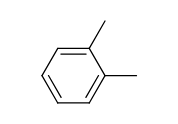
\includegraphics{smile-332d2586713d7a4857fe03cacd56f36c3681f473}\\
A) 1.2-dimetilbenzol\\
B) $1.1^{-}$ dimetilbenzol\\
C) 1.3-dimetilbenzol dimetilbenzol\\
D) $1.4^{-}$\\
2. Quyidagi rasmda ko'rsatilgan benzol gomologini sistematik nomenklatura bo'yicha nomlang.\\
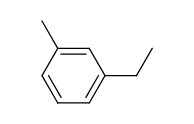
\includegraphics{smile-6f86e7ace3b936043e6826dd405aed27eecdad23}\\
A) 3-metil-1-propilbenzol\\
B) 1-metil-2-propilbenzol\\
C) 2-metil-3-propilbenzol\\
D) 1-metil-3-propilbenzol\\
3. Quyidagi rasmda ko'rsatilgan benzol gomologini sistematik nomenklatura bo'yicha nomlang.\\
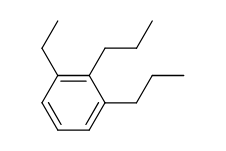
\includegraphics{smile-d9ebc1b306eaceca04cc94ba4352d8a438f0fc7e}\\
A) 1.3-dietil-3-propilbenzol\\
B) 1.2-dietil-3-propilbenzol\\
C) 2.3-dietil-1-propilbenzol\\
D) 1.2 -dietil-4-propilbenzol\\
4. Quyidagi rasmda ko'rsatilgan benzol gomologini sistematik nomenklatura bo'yicha nomlang.\\
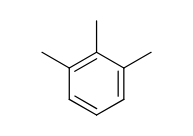
\includegraphics{smile-e4e8ee60606d912921d1376848a1a8a9f1e34bab}\\
A) 1.2.4-trimetilbenzol\\
B) 1.2.2-trimetilbenzol\\
C) 1.2.3-trimetilbenzol\\
D) 1.3.3-trimetilbenzol\\
5. Quyidagi rasmda ko'rsatilgan benzol gomologini sistematik nomenklatura bo'yicha nomlang.\\
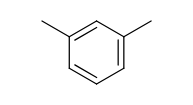
\includegraphics{smile-d7df328d45dcd3f892bf5b11abd7693569f69bc2}\\
A) 1.4-dimetil-3-propilbenzol\\
B) 1.3-dimetil-2-propilbenzol\\
C) 1.2-dimetil-4-propilbenzol\\
D) 1.3-dimetil-5-propilbenzol\\
6. Quyidagi rasmda ko'rsatilgan benzol gomologini sistematik nomenklatura bo'yicha nomlang.\\
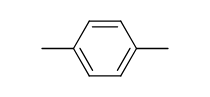
\includegraphics{smile-853d14a4fb5b6600a32dc20c41824260b3a8357d}\\
A) 1.2-dimetilbenzol B) 1.1 -dimetilbenzol\\
C) 1.3-dimetilbenzol D) 1.4-dimetilbenzol\\
7. Quyidagi rasmda ko'rsatilgan benzol gomologini sistematik nomenklatura bo'yicha nomlang.\\
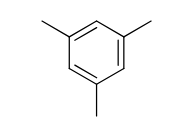
\includegraphics{smile-460e091dc223882c2fb2e2eef01ee7b96ff8061c}\\
A) 1.3.5-trimetilbenzol\\
B) 1.3.4-trimetilbenzol\\
C) 1.2.5-trimetilbenzol\\
D) 1.3.6-trimetilbenzol\\
8. Quyidagi rasmda ko'rsatilgan benzol gomologini sistematik nomenklatura bo'yicha nomlang.\\
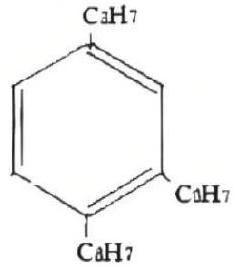
\includegraphics[max width=\textwidth, center]{2025_08_11_1fac7286a628a1b4eedag-74}\\
A) 1.2.5-tripropilbenzol\\
B) 1.2.4-tripropilbenzol\\
C) 1.3.4-tripropilbenzol\\
D) 1.3.5-tripropilbenzol\\
9. Quyidagi rasmda ko'rsatilgan benzol gomologini sistematik nomenklatura bo'yicha nomlang.\\
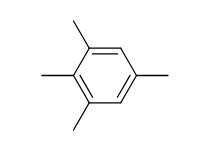
\includegraphics{smile-50e9185f02af0d929f0942a9eb8585a4722c49a4}\\
A) 1.2.3.5-tetrametilbenzol\\
B) 1.2.3.6-tetrametilbenzol\\
C) 1.4.3.5-tetrametilbenzol\\
D) 1.2.3.4-tetrametilbenzol\\
10. Quyidagi rasmda ko'rsatilgan benzol gomologini sistematik nomenklatura bo'yicha nomlang.\\
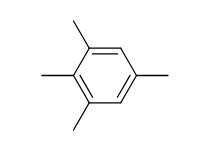
\includegraphics{smile-437c1a04ecbaf6400097e62e8c452b1b84d1133b}\\
A) 1.2.3-trimetil-5-propilbenzol\\
B) 1.2.3-trimetil-5-propilbenzol\\
C) 1.2 .3 -trimetil- 5 -propilbenzol\\
D) 1.2 .3 -trimetil- 5 -propilbenzol
  \item Siklogeksandan benzol olish reaksiyasi natijasida da o'lchangan 67,2 litr vodorod ajralib chiqqan bo'lsa necha ml benzol hosil bo'lgan. (benzolning zichligi $0,78 \mathrm{~g} / \mathrm{ml}$ )\\
A) 78\\
B) 100\\
C) 94\\
D) 156
  \item Siklogeksandan benzol olish reaksiyasi natijasida da o'lchangan 33,6 litr vodorod ajralib chiqqan bo'lsa necha ml benzol hosil bo'lgan. (benzolning zichligi $0,78 \mathrm{~g} / \mathrm{ml}$ )\\
A) 50\\
B) 100\\
C) 150\\
D) 200
  \item Siklogeksandan benzol olish reaksiyasi natijasida da o'lchangan 6,72 litr vodorod ajralib chiqqan bo'lsa necha ml benzol hosil bo'lgan. (benzolning zichligi $0,78 \mathrm{~g} / \mathrm{ml}$ )\\
A) 8\\
B) 9\\
C) 12\\
D) 10
  \item Siklogeksandan benzol olish reaksiyasi natijasida da o'lchangan 13,44 litr vodorod ajralib chiqqan bo'lsa necha ml benzol hosil bolgan. (benzolning zichligi $0,78 \mathrm{~g} / \mathrm{ml}$ )\\
A) 15\\
B) 20\\
C) 14\\
D) 12
  \item Siklogeksandan benzol olish reaksiyasi natijasida da o'lchangan 134,4 litr vodorod ajralib chiqqan bo'lsa necha ml benzol hosil bo'lgan. (benzolning zichligi $0,78 \mathrm{~g} / \mathrm{ml}$ )\\
A) 140\\
B) 150\\
C) 180\\
D) 200
  \item Metilsiklogeksandan toluol olish reaksiyasi natijasida da o'lchangan 67,2 litr vodorod ajralib chiqqan bo'lsa necha ml benzol hosil bo'lgan. (benzolning zichligi $0,92 \mathrm{~g} / \mathrm{ml}$ )\\
A) 92\\
B) 100\\
C) 184\\
D) 156
  \item Metilsiklogeksandan toluol olish reaksiyasi natijasida da o'lchangan 26,88 litr vodorod ajralib chiqqan bo'lsa nechá ml benzol hosil bo'lgan. (benzolning zichligi $0,92 \mathrm{~g} / \mathrm{ml}$ )\\
A) 70\\
B) 50\\
C) 60\\
D) 40
  \item Metilsiklogeksandan toluol olish reaksiyasi natijasida da o'lchangan 20,16 litr vodorod ajralib chiqqan bo'lsa necha ml benzol hosil bo'lgan. (benzolning zichligi $0,92 \mathrm{~g} / \mathrm{ml}$ )\\
A) 30\\
B) 40\\
C) 50\\
D) 60
  \item Metilsiklogeksandan toluol olish reaksiyasi natijasida da o'lchangan 134,4 litr vodorod ajralib chiqqan bo'lsa necha ml benzol hosil bo'lgan. (benzolning zichligi $0,92 \mathrm{~g} / \mathrm{ml}$ )\\
A) 150\\
B) 200\\
C) 180\\
D) 190
  \item Metilsiklogeksandan toluol olish reaksiyasi natijasida da o'lchangan 168 litr vodorod ajralib chiqqan bo'lsa necha ml benzol hosil bo'lgan. (benzolning zichligi $0,92 \mathrm{~g} / \mathrm{ml}$ )\\
A) 250\\
B) 210\\
C) 194\\
D) 156
  \item $\mathrm{CaC}_{2}$ dan ikki boshqichda benzol sintez qilinadi. $64 \mathrm{~g} \mathrm{CaC}_{2}$ dan necha g benzol sintez qilingan? ( reaksiya unumi mos ravishda birinchi va ikkinchi boshqich uchun $50 \%$ va $80 \%$ ga teng)\\
A) 13\\
B) 10,4\\
C) 5,2\\
D) 7,8
  \item $\mathrm{CaC}_{2}$ dan ikki boshqichda benzol sintez qilinadi. $32 \mathrm{~g} \mathrm{CaC}_{2}$ dan necha g benzol sintez qilingan? ( reaksiya unumi mos ravishda birinchi va ikkinchi boshqich uchun $40 \%$ va $50 \%$ ga teng)\\
A) 1,3\\
B) 2,6\\
C) 5,2\\
D) 7,8
  \item $\mathrm{Ca} \mathrm{C}_{2}$ dan ikki boshqichda benzol sintez qilinadi. $128 \mathrm{~g} \mathrm{CaC}_{2}$ dan necha g benzol sintez qilingan? (reaksiya unumi mos ravishda birinchi va ikkinchi boshqich uchun $50 \%$ va $100 \%$ ga teng)\\
A) 26\\
B) 104\\
C) 52\\
D) 78
  \item $\mathrm{CaC}_{2}$ dan ikki boshqichda benzol sintez qilinadi. $192 \mathrm{~g} \mathrm{CaC}_{2}$ dan necha g benzol sintez qilingan? ( reaksiya unumi mos ravishda birinchi va ikkinchi boshqich uchun $80 \%$ va $80 \%$ ga teng)\\
A) 28,84\\
B) 54,28 ।\\
C) 54,44\\
D) 49,92
  \item $\mathrm{CaC}_{2}$ dan ikki boshqichda benzol sintez qilinadi. $96 \mathrm{~g} \mathrm{CaC}_{2}$ dan necha g benzol sintez qilingan? ( reaksiya unumi mos ravishda birinchi va ikkinchi boshqich uchun $50 \%$ va $40 \%$ ga teng)\\
A) 13\\
B) 10,4\\
C) 5,2\\
D) 7,8
  \item $\mathrm{CaC}_{2}$ dan ikki boshqichda benzol sintez qilinadi. $12,8 \mathrm{~g} \mathrm{CaC}_{2}$ dan necha g benzol sintez qilingan? ( reaksiya unumi mos ravishda birinchi va ikkinchi boshqich uchun $80 \%$ va $100 \%$ ga teng)\\
A) 5,2\\
B) 6,44\\
C) 4,16\\
D) 7,8
  \item $\mathrm{CaC}_{2}$ dan ikki boshqichda benzol sintez qilinadi. $16 \mathrm{~g} \mathrm{CaC}_{2}$ dan necha g benzol sintez qilingan? (reaksiya unumi mos ravishda birinchi va ikkinchi boshqich uchun $50 \%$ va $90 \%$ ga teng)\\
A) 12,42\\
B) 10,43\\
C) 5,85\\
D) 2,925
  \item $\mathrm{CaC}_{2}$ dan ikki boshqichda benzol sintez qilinadi. $25,6 \mathrm{~g} \mathrm{CaC}_{2}$ dan necha g benzol sintez qilingan? ( reaksiya unumi mos ravishda birinchi va ikkinchi boshqich uchun $100 \%$ va $80 \%$ ga teng)\\
A) 8,32\\
B) 4,16\\
C) 5,2\\
D) 10,4
  \item $\mathrm{CaC}_{2}$ dan ikki boshqichda benzol sintez qilinadi. $256 \mathrm{~g} \mathrm{CaC}_{2}$ dan necha g benzol sintez qilingan? ( reaksiya unumi mos ravishda birinchi va ikkinchi boshqich uchun $50 \%$ va $80 \%$ ga teng)\\
A) 83,2\\
B) 41,6\\
C) 52\\
D) 104
  \item $\mathrm{CaC}_{2}$ dan ikki boshqichda benzol sintez qilinadi. $128 \mathrm{~g} \mathrm{CaC}_{2}$ dan necha g benzol sintez qilingan? ( reaksiya unumi mos ravishda birinchi va ikkinchi boshqich uchun $100 \%$ val00 \% ga teng)\\
A) 13\\
B) 104\\
C) 52\\
D) 78
  \item Toluol kislotali $\left(\mathrm{H}_{2} \mathrm{SO}_{4}\right)$ muhitda $\mathrm{KMnO}_{4}$ bilan oksidlanganda benzoy kislota hosil bo'ladi. Ushbu reaksiya bo'yicha 92 g toluoldan $80 \%$ unum bilan necha g benzoy kislota olish mumkin?\\
A) 97,6\\
B) 122\\
C) 48,8\\
D) 92
  \item Toluol kislotali $\left(\mathrm{H}_{2} \mathrm{SO}_{4}\right)$ muhitda $\mathrm{KMnO}_{4}$ bilan oksidlanganda benzoy kislota hosil bo'ladi. Ushbu reaksiya\\
bo'yicha 184 g toluoldan $50 \%$ unum bilan necha g benzoy kislota olish mumkin?\\
A) 97,6\\
B) 122\\
C) 48,8\\
D) 92
  \item Toluol kislotali $\left(\mathrm{H}_{2} \mathrm{SO}_{4}\right)$ muhitda $\mathrm{KMnO}_{4}$ bilan oksidlanganda benzoy kislota hosil bo'ladi. Ushbu reaksiya bo'yicha $18,4 \mathrm{~g}$ toluoldan $40 \%$ unum bilan necha g benzoy kislota olish mumkin?\\
A) 9,76\\
B) 12,2\\
C) 4,88\\
D) 9,2
  \item Toluol kislotali $\left(\mathrm{H}_{2} \mathrm{SO}_{4}\right)$ muhitda $\mathrm{KMnO}_{4}$ bilan oksidlanganda benzoy kislota hosil bo'ladi. Ushbu reaksiya bo'yicha 276 g toluoldan $50 \%$ unum bilan necha g benzoy kislota olish mumkin?\\
A) 976\\
B) 122\\
C) 366\\
D) 183
  \item Toluol kislotali $\left(\mathrm{H}_{2} \mathrm{SO}_{4}\right)$ muhitda $\mathrm{KMnO}_{4}$ bilan oksidlanganda benzoy kislota hosil bo'ladi. Ushbu reaksiya bo'yicha 92 g toluoldan $100 \%$ unum bilan necha g benzoy kislota olish mumkin?\\
A) 97,6\\
B) 122\\
C) 48,8\\
D) 92
  \item Toluol kislotali $\left(\mathrm{H}_{2} \mathrm{SO}_{4}\right)$ muhitda $\mathrm{KMnO}_{4}$ bilan oksidlanganda benzoy kislota hosil bo'ladi. Ushbu reaksiya bo'yicha $36,8 \mathrm{~g}$ toluoldan $40 \%$ unum bilan necha g benzoy kislota olish mumkin?\\
A) 19,76\\
B) 19,52\\
C) 48,8\\
D) 12,2
  \item Toluol kislotali $\left(\mathrm{H}_{2} \mathrm{SO}_{4}\right)$ muhitda $\mathrm{KMnO}_{4}$ bilan oksidlanganda benzoy kislota hosil bo'ladi. Ushbu reaksiya bo'yicha 46 g toluoldan $50 \%$ unum bilan necha g benzoy kislota olish mumkin?\\
A) 61\\
B) 12,2\\
C) 122\\
D) 30,5
  \item Toluol kislotali $\left(\mathrm{H}_{2} \mathrm{SO}_{4}\right)$ muhitda $\mathrm{KMnO}_{4}$ bilan oksidlanganda benzoy kislota hosil bo'ladi. Ushbu reaksiya bo'yicha 46 g toluoldan $100 \%$ unum bilan necha g benzoy kislota olish mumkin?\\
A) 97,6\\
B) 12,2\\
C) 122\\
D) 61
  \item Toluol kislotali $\left(\mathrm{H}_{2} \mathrm{SO}_{4}\right)$ muhitda $\mathrm{KMnO}_{4}$ bilan oksidlanganda benzoy kislota hosil bo'ladi. Ushbu reaksiya bo'yicha 23 g toluoldan $50 \%$ unum bilan necha g benzoy kislota olish mumkin?\\
A) 15,25\\
B) 12,2\\
C) 4,88\\
D) 9,2
  \item Toluol kislotali $\left(\mathrm{H}_{2} \mathrm{SO}_{4}\right)$ muhitda $\mathrm{KMnO}_{4}$ bilan oksidlanganda benzoy kislota hosil bo'ladi. Ushbu reaksiya bo'yicha 184 g toluoldan $100 \%$ unum bilan necha g benzoy kislota olish mumkin?\\
A) 122\\
B) 183\\
C) 366\\
D) 244
  \item $7,8 \mathrm{~g}$ benzol katalizator ishtirokida monoxlorlanish reaksiyasiga kirishdi. Reaksiya natijasida xosil bo'lgan kislota necha g $20 \%$ li NaOH eritmasini to'liq neytrallashga yetadi?\\
A) 20\\
B) 40\\
C) 30\\
D) 60
  \item 39 g benzol katalizator ishtirokida monoxlorlanish reaksiyasiga kirishdi. Reaksiya natijasida xosil bo'lgan kislota necha g $40 \%$ li NaOH eritmasini to'liq neytrallashga yetadi?\\
A) 20\\
B) 30\\
C) 40\\
D) 50
  \item 78 g benzol katalizator ishtirokida monoxlorlanish reaksiyasiga kirishdi. Reaksiya natijasida xosil bo'lgan kislota necha g $10 \%$ li NaOH eritmasini to'liq neytrallashga yetadi?\\
A) 200\\
B) 400\\
C) 300\\
D) 600
  \item $15,6 \mathrm{~g}$ benzol katalizator ishtirokida monoxlorlanish reaksiyasiga kirishdi. Reaksiya natijasida xosil bo'lgan kislota necha g $25 \%$ li NaOH eritmasini to'liq neytrallashga yetadi?\\
A) 32\\
B) 48\\
C) 64\\
D) 80
  \item $3,9 \mathrm{~g}$ benzol katalizator ishtirokida monoxlorlanish reaksiyasiga kirishdi. Reaksiya natijasida xosil bo'lgan kislota necha g $40 \%$ li NaOH eritmasini to'liq neytrallashga yetadi?\\
A) 2\\
B) 3\\
C) 5\\
D) 4
  \item 156 g benzol katalizator ishtirokida monoxlorlanish reaksiyasiga kirishdi. Reaksiya natijasida xosil bo'lgan kislota necha g $50 \%$ li NaOH eritmasini to'liq neytrallashga yetadi?\\
A) 160\\
B) 200\\
C) 80\\
D) 120
  \item $31,2 \mathrm{~g}$ benzol katalizator ishtirokida monoxlorlanish reaksiyasiga kirishdi. Reaksiya natijasida xosil bo'lgan kislota necha g $25 \%$ li NaOH eritmasini to'liq neytrallashga yetadi?\\
A) 32\\
B) 48\\
C) 64\\
D) 16
  \item $23,4 \mathrm{~g}$ benzol katalizator ishtirokida monoxlorlanish reaksiyasiga kirishdi. Reaksiya natijasida xosil bo'lgan kislota necha g $50 \%$ li NaOH eritmasini to'liq neytrallashga yetadi?\\
A) 24\\
B) 48\\
C) 12\\
D) 16
  \item 39 g benzol katalizator ishtirokida monoxlorlanish reaksiyasiga kirishdi. Reaksiya natijasida xosil bo'lgan kislota necha g $25 \%$ li NaOH eritmasini to'liq neytrallashga yetadi?\\
A) 160\\
B) 200\\
C) 80\\
D) 120
  \item 78 g benzol katalizator ishtirokida monoxlorlanish reaksiyasiga kirishdi. Reaksiya natijasida xosil bo'lgan kislota necha g $20 \%$ li NaOH eritmasini to'liq neytrallashga yetadi?\\
A) 160\\
B) 200\\
C) 80\\
D) 120
  \item $1,2 \mathrm{~g}$ benzol gomologi konsentirlangan sulfat kislota ishtirokida nitrolanganda 50 $\%$ unum bilan $0,825 \mathrm{~g}$ mononitro birikmalar aralashmasi hosil bo'ldi.\\
Reaksiya uchun olingan benzol gomologini aniqlang.\\
A) $\mathrm{C}_{6} \mathrm{H}_{6}$\\
B) $\mathrm{C}_{7} \mathrm{H}_{8}$\\
C) $\mathrm{C}_{8} \mathrm{H}_{10}$\\
D) $\mathrm{C}_{9} \mathrm{H}_{12}$
  \item $1,84 \mathrm{~g}$ benzol gomologi konsentirlangan sulfat kislota ishtirokida nitrolanganda $60 \%$ unum bilan $1,644 \mathrm{~g}$ mononitro birikmalar aralashmasi hosil bo'ldi. Reaksiya uchun olingan benzol gomologini aniqlang.\\
A) $\mathrm{C}_{6} \mathrm{H}_{6}$\\
B) $\mathrm{C}_{7} \mathrm{H}_{8}$\\
C) $\mathrm{C}_{8} \mathrm{H}_{10}$\\
D) $\mathrm{C}_{9} \mathrm{H}_{12}$
  \item $9,75 \mathrm{~g}$ benzol gomologi konsentirlangan sulfat kislota ishtirokida nitrolanganda $80 \%$ unum bilan $12,3 \mathrm{~g}$ mononitro birikmalar aralashmasi hosil bo'ldi. Reaksiya uchun olingan benzol gomologini aniqlang.\\
A) $\mathrm{C}_{6} \mathrm{H}_{6}$\\
B) $\mathrm{C}_{7} \mathrm{H}_{8}$\\
C) $\mathrm{C}_{8} \mathrm{H}_{10}$\\
D) $\mathrm{C}_{9} \mathrm{H}_{12}$
  \item $1,06 \mathrm{~g}$ benzol gomologi konsentirlangan sulfat kislota ishtirokida nitrolanganda $100 \%$ unum bilan $1,51 \mathrm{~g}$ mononitro birikmalar aralashmasi hosil bo'ldi. Reaksiya uchun olingan benzol gomologini aniqlang.\\
A) $\mathrm{C}_{6} \mathrm{H}_{6}$\\
B) $\mathrm{C}_{7} \mathrm{H}_{8}$\\
C) $\mathrm{C}_{8} \mathrm{H}_{10}$\\
D) $\mathrm{C}_{9} \mathrm{H}_{12}$
  \item 6 g benzol gomologi konsentirlangan sulfat kislota ishtirokida nitrolanganda 40 $\%$ unum bilan $3,3 \mathrm{~g}$ mononitro birikmalar aralashmasi hosil bo'ldi. Reaksiya uchun olingan benzol gomologini aniqlang.\\
A) $\mathrm{C}_{6} \mathrm{H}_{6}$\\
B) $\mathrm{C}_{7} \mathrm{H}_{8}$\\
C) $\mathrm{C}_{8} \mathrm{H}_{10}$\\
D) $\mathrm{C}_{9} \mathrm{H}_{12}$
  \item $2,12 \mathrm{~g}$ benzol gomologi konsentirlangan sulfat kislota ishtirokida nitrolanganda $50 \%$ unum bilan $1,51 \mathrm{~g}$ mononitro birikmalar aralashmasi hosil bo'ldi. Reaksiya uchun olingan benzol gomologini aniqlang.\\
A) $\mathrm{C}_{6} \mathrm{H}_{6}$\\
B) $\mathrm{C}_{7} \mathrm{H}_{8}$\\
C) $\mathrm{C}_{8} \mathrm{H}_{10}$\\
D) $\mathrm{C}_{9} \mathrm{H}_{12}$
  \item 156 g benzol gomologi konsentirlangan sulfat kislota ishtirokida nitrolanganda 50 $\%$ unum bilan 123 g mononitro birikmalar aralashmasi hosil bo'ldi. Reaksiya uchun olingan benzol gomologini aniqlang.\\
A) $\mathrm{C}_{6} \mathrm{H}_{6}$\\
B) $\mathrm{C}_{7} \mathrm{H}_{8}$\\
C) $\mathrm{C}_{8} \mathrm{H}_{10}$\\
D) $\mathrm{C}_{9} \mathrm{H}_{12}$
  \item $0,6 \mathrm{~g}$ benzol gomologi konsentirlangan sulfat kislota ishtirokida nitrolanganda 80 $\%$ unum bilan $0,66 \mathrm{~g}$ mononitro birikmalar\\
aralashmasi hosil bo'ldi. Reaksiya uchun olingan benzol gomologini aniqlang.\\
A) $\mathrm{C}_{6} \mathrm{H}_{6}$\\
B) $\mathrm{C}_{7} \mathrm{H}_{8}$\\
C) $\mathrm{C}_{8} \mathrm{H}_{10}$\\
D) $\mathrm{C}_{4} \mathrm{H}_{12}$
  \item $18,4 \mathrm{~g}$ benzol gomologi konsentirlangan sulfat kislota ishtirokida nitrolanganda $40 \%$ unum bilan $10,96 \mathrm{~g}$ mononitro birikmalar aralashmasi hosil bo'ldi. Reaksiya uchun olingan benzol gomologini aniqlang.\\
A) $\mathrm{C}_{6} \mathrm{H}_{6}$\\
B) $\mathrm{C}_{7} \mathrm{H}_{8}$\\
C) $\mathrm{C}_{8} \mathrm{H}_{10}$\\
D) $\mathrm{C}_{9} \mathrm{H}_{12}$
  \item $2,4 \mathrm{~g}$ benzol gomologi konsentirlangan sulfat kislota ishtirokida nitrolanganda 60 $\%$ unum bilan $1,98 \mathrm{~g}$ mononitro birikmalar aralashmasi hosil bo'ldi. Reaksiya uchun olingan benzol gomologini aniqlang.\\
A) $\mathrm{C}_{6} \mathrm{H}_{6}$\\
B) $\mathrm{C}_{7} \mathrm{H}_{8}$\\
C) $\mathrm{C}_{8} \mathrm{H}_{10}$\\
D) $\mathrm{C}_{9} \mathrm{H}_{12}$
  \item Benzol va toluoldan iborat $24,8 \mathrm{~g}$ aralashma $200 \mathrm{~g} 24 \%$ li bromli suvni rangsizlantirsa, aralashma tarkibida necha g benzol bor?\\
A) 15,6\\
B) 7,8\\
C) 3,9\\
D) 23,4
  \item Benzol va toluoldan iborat 17 g aralashma $1000 \mathrm{~g} 4,8 \%$ li bromli suvni rangsizlantirsa, aralashma tarkibida necha g benzol bor?\\
A) 15,6\\
B) 7,8\\
C) 3,9\\
D) 23,4
  \item Benzol va toluoldan iborat $49,6 \mathrm{~g}$ aralashma $500 \mathrm{~g} 19,2 \%$ li bromli suvni rangsizlantirsa, aralashma tarkibida necha g benzol bor?\\
A) 15,6\\
B) 39\\
C) 31,2\\
D) 23,4
  \item Benzol va toluoldan iborat $60,2 \mathrm{~g}$ aralashma $1000 \mathrm{~g} 19,2 \%$ li bromli suvni rangsizlantirsa, aralashma tarkibida necha g benzol bor?\\
A) 15,6\\
B) 31,2\\
C) 39\\
D) 23,4
  \item Benzol va toluoldan iborat $92,8 \mathrm{~g}$ aralashma $1000 \mathrm{~g} 24 \%$ li bromli suvni\\
rangsizlantirsa, aralashma tarkíbida necha g benzol bor?\\
A) 46,8\\
B) 39\\
C) 15,6\\
D) 23,4
  \item Benzol va toluoldan iborat 51 g aralashma $200 \mathrm{~g} 72 \%$ li bromli suvní rangsizlantirsa, aralashma tarkibida necha g benzol bor?\\
A) 15,6\\
B) 7,8\\
C) 3,9\\
D) 23,4
  \item Benzol va toluoldan iborat $58,8 \mathrm{~g}$ aralashma $1000 \mathrm{~g} 14,4 \%$ li bromli suvní rangsizlantirsa, aralashma tarkibida necha g benzol bor?\\
A) 19,5\\
B) 39\\
C) 31,2\\
D) 23,4
  \item Benzol va toluoldan iborat 119 g aralashma $1000 \mathrm{~g} 33,6 \%$ li bromli suvni rangsizlantirsa, aralashma tarkibida necha g benzol bor?\\
A) 31,2\\
B) 54,6\\
C) 23,4\\
D) 39
  \item Benzol va toluoldan iborat $76,5 \mathrm{~g}$ aralashma 1000 g 21,6 \% li bromli suvni rangsizlantirsa, aralashma tarkibida necha g benzol bor?\\
A) 54,6\\
B) 23,4\\
C) 31,2\\
D) 35,1
  \item Benzol va toluoldan iborat $42,5 \mathrm{~g}$ aralashma $500 \mathrm{~g} 24 \%$ li bromli suvni rangsizlantirsa, aralashma tarkibida necha $g$ benzol bor?\\
A) 19,5\\
B) 78\\
C) 39\\
D) 23,4
  \item 17 g benzol va toluoldan iborat aralashmani to'liq yondirish uchun $52,8 \mathrm{~g}$ ozon-kislorod aralashmasi sarflangan bo'lsa aralashma tarkibidagi toluol massasini (g) hisoblang.\\
A) 9,2\\
B) 4,6\\
C) 2,3\\
D) 4,9
  \item $43,2 \mathrm{~g}$ benzol va toluoldan iborat aralashmani to'liq yondirish uchun $134,4 \mathrm{~g}$ ozon-kislorod aralashmasi sarflangan bo'lsa aralashma tarkibidagi toluol massasini (g) hisoblang.\\
A) 18,4\\
B) 9,2\\
C) 27,6\\
D) 36,8
  \item $44,6 \mathrm{~g}$ benzol va toluoldan iborat aralashmani to'liq yondirish uchun $139,2 \mathrm{~g}$ ozon-kislorod aralashmasi sarflangan bo'lsa aralashma tarkibidagi toluol massasini (g) hisoblang.\\
A) 18,4\\
B) 9,2\\
C) 27,6\\
D) 36,8
  \item 51 g benzol va toluoldan iborat aralashmani to'liq yondirish uchun $158,4 \mathrm{~g}$ ozon-kislorod aralashmasi sarflangan bo'lsa aralashma tarkibidagi toluol massasini (g) hisoblang.\\
A) 18,4\\
B) 9,2\\
C) 27,6\\
D) 36.8
  \item $40,4 \mathrm{~g}$ benzol va toluoldan iborat aralashmani to'liq yondirish uchun $124,8 \mathrm{~g}$ ozon-kislorod aralashmasi sarflangan bo'lsa aralashma tarkibidagi toluol massasini (g) hisoblang.\\
A) 9,2\\
B) 4,6\\
C) 2,3\\
D) 4,9
  \item $53,8 \mathrm{~g}$ benzol va toluoldan iborat aralashmani to'liq yondirish uchun 168 g ozon-kislorod aralashmasi sarflangan bo'lsa aralashma tarkibidagi benzol massasini (g) hisoblang.\\
A) 15,6\\
B) 3,9\\
C) 7,8\\
D) 39
  \item 85 g benzol va toluoldan iborat aralashmani to'liq yondirish uchun 264 g ozon-kislorod aralashmasi sarflangan bo'lsa aralashma tarkibidagi benzol massasini ( g ) hisoblang.\\
A) 15,6\\
B) 3,9\\
C) 7,8\\
D) 39
  \item $75,8 \mathrm{~g}$ benzol va toluoldan iborat aralashmani to'liq yondirish uchun $235,2 \mathrm{~g}$ ozon-kislorod aralashmasi sarflangan\\
bo'lsa aralashma tarkibidagi benzol massasini (g) hisoblang.\\
A) 15,6\\
B) 3,9\\
C) 7.8\\
D) 39
  \item $52,4 \mathrm{~g}$ benzol va toluoldan iborat aralashmani to'liq yondirish uchun 163.2 g ozon-kislorod aralashmasi sarflangan bo'lsa aralashma tarkibidagi benzol massasini (g) hisoblang.\\
A) 15,6\\
B) 3,9\\
C) 7,8\\
D) 39
  \item $70,8 \mathrm{~g}$ benzol va toluoldan iborat aralashmani to'liq yondirish uchun $220,8 \mathrm{~g}$ ozon-kislorod aralashmasi sarflangan bo'lsa aralashma tarkibidagi benzol massasini (g) hisoblang.\\
A) 15,6\\
B) 3,9\\
C) 7,8\\
D) 39
  \item 100 ml zichligi $0,832 \mathrm{~g} / \mathrm{ml}$ bo'lgan stirolning benzoldagi eritmasi $1000 \mathrm{~g} 8 \%$ li bromli suvni rangsizlantirsa, stirolning eritmadagi foiz konsentratsiyasini aniqlang.\\
A) 62,5\\
B) 78\\
C) 42,4\\
D) 50
  \item 100 ml zichligi $0,884 \mathrm{~g} / \mathrm{ml}$ bo'lgan stirolning benzoldagi eritmasi $1000 \mathrm{~g} 6,4$ \% li bromli suvni rangsizlantirsa, stirolning eritmadagi foiz konsentratsiyasini aniqlang.\\
A) 53\\
B) 46\\
C) 47\\
D) 54
  \item 160 ml zichligi $0,8125 \mathrm{~g} / \mathrm{ml}$ bo'lgan stirolning benzoldagi eritmasi $1000 \mathrm{~g} 12,8$ \% li bromli suvni rangsizlantirsa, stirolning eritmadagi foiz konsentratsiyasini aniqlang.\\
A) 55\\
B) 45\\
C) 36\\
D) 64
  \item 150 ml zichligi $0,728 \mathrm{~g} / \mathrm{ml}$ bo'lgan stirolning benzoldagi eritmasi $1000 \mathrm{~g} 9,6$ \% li bromli suvni rangsizlantirsa, stirolning eritmadagi foiz konsentratsiyasini aniqlang.\\
A) 46\\
B) 57\\
C) 43\\
D) 44
  \item 100 ml zichligi $0,91 \mathrm{~g} / \mathrm{ml}$ bo'lgan stirolning benzoldagi eritmasi $1000 \mathrm{~g} 8 \%$ li bromli suvni rangsizlantirsa, stirolning eritmadagi foiz konsentratsiyasini aniqlang.\\
A) 46\\
B) 57\\
C) 43\\
D) 44
  \item 160 ml zichligi $0,65 \mathrm{~g} / \mathrm{ml}$ bo'lgan stirolning benzoldagi eritmasi $1000 \mathrm{~g} 6,4$ \% li bromli suvni rangsizlantirsa, stirolning eritmadagi foiz konsentratsiyasini aniqlang.\\
A) 62\\
B) 38\\
C) 40\\
D) 60
  \item 100 ml zichligi $0,78 \mathrm{~g} / \mathrm{ml}$ bo'lgan stirolning benzoldagi eritmasi 1000 g 4,8 \% li bromli suvni rangsizlantirsa, stirolning eritmadagi foiz konsentratsiyasini aniqlang.\\
A) 62\\
B) 38\\
C) 40\\
D) 60
  \item 200 ml zichligi $0,637 \mathrm{~g} / \mathrm{ml}$ bo'lgan stirolning benzoldagi eritmasi $1000 \mathrm{~g} 11,2$ \% li bromli suvni rangsizlantirsa, stirolning eritmadagi foiz konsentratsiyasini aniqlang.\\
A) 46\\
B) 57\\
C) 43\\
D) 44
  \item 200 ml zichligi $0,533 \mathrm{~g} / \mathrm{ml}$ bo'lgan stirolning benzoldagi eritmasi $1000 \mathrm{~g} 8 \%$ li bromli suvni rangsizlantirsa, stirolning eritmadagi foiz konsentratsiyasini aniqlang.\\
A) 62,5\\
B) 48,8\\
C) 42,4\\
D) 51,2
  \item 150 ml zichligi $0,78 \mathrm{~g} / \mathrm{ml}$ bo'lgan stirolning benzoldagi eritmasi $1000 \mathrm{~g} 8 \%$ li bromli suvni rangsizlantirsa, stirolning eritmadagi foiz konsentratsiyasini aniqlang.\\
A) 62,5\\
B) 44,4\\
C) 42,4\\
D) 53,33
  \item Molekulasi tarkibida 66 ta proton saqlagan benzol gomologi to'liq yonishidan hosil bo'lgan $\mathrm{CO}_{2} 200 \mathrm{~g} 36 \%$ li NaOH eritmasini to'la neytrallashga yetarli bo'lsa, reaksiya uchun necha g aren olingan?\\
A) 12\\
B) 24\\
C) 36\\
D) 48
  \item Molekulasi tarkibida 50 ta proton saqlagan benzol gomologi to'liq yonishidan hosil bo'lgan $\mathrm{CO}_{2} 200 \mathrm{~g} 56 \%$ li NaOH eritmasini to'la neytrallashga yetarli bo'lsa, reaksiya uchun necha $g$ aren olingan?\\
A) 36,8\\
B) 9,2\\
C) 18,4\\
D) 4,6
  \item Molekulasi tarkibida 42 ta proton saqlagan benzol gomologi to'liq yonishidan hosil bo'lgan $\mathrm{CO}_{2} 200 \mathrm{~g} 72 \%$ li NaOH eritmasini to'la neytrallashga yetarli bo'lsa, reaksiya uchun necha g aren olingan?\\
A) 15,6\\
B) 23,4\\
C) 39\\
D) 7,8
  \item Molekulasi tarkibida 58 ta proton saqlagan benzol gomologi to'liq yonishidan hosil bo'lgan $\mathrm{CO}_{2} 200 \mathrm{~g} 32 \%$ li NaOH eritmasini to'la neytrallashga yetarli bo'lsa, reaksiya uchun necha $g$ aren olingan?\\
A) 10,6\\
B) 5,3\\
C) 21,2\\
D) 42,4
  \item Molekulasi tarkibida 66 ta proton saqlagan benzol gomologi to'liq yonishidan hosil bo'lgan $\mathrm{CO}_{2} 200 \mathrm{~g} 54 \%$ li NaOH eritmasini to'la neytrallashga yetarli bo'lsa, reaksiya uchun necha $g$ aren olingan?\\
A) 12\\
B) 24\\
C) 18\\
D) 6
  \item Molekulasi tarkibida 50 ta proton saqlagan benzol gomologi to'liq yonishidan hosil bo'lgan $\mathrm{CO}_{2} 200 \mathrm{~g} 28 \%$ li NaOH eritmasini to'la neytrallashga yetarli\\
bo'lsa, reaksiya uchun necha g aren olingan?\\
A) 36,8\\
B) 9,2\\
C) 18,4\\
D) 4,6
  \item Molekulasi tarkibida 42 ta proton saqlagan benzol gomologi to'liq yonishidan hosil bo'lgan $\mathrm{CO}_{2} 200 \mathrm{~g} 24 \%$ li NaOH eritmasini to'la neytrallashga yetarli bo'lsa, reaksiya uchun necha g aren olingan?\\
A) 15,6\\
B) 23,4\\
C) 39\\
D) 7,8
  \item Molekulasi tarkibida 50 ta proton saqlagan benzol gomologi to'liq yonishidan hosil bo'lgan $\mathrm{CO}_{2} 200 \mathrm{~g} 42 \%$ li NaOH eritmasini to'la neytrallashga yetarli bo'lsa, reaksiya uchun necha g aren olingan\\
A) 13,8\\
B) 27,6\\
C) 9,2\\
D) 18,4
  \item Molekulasi tarkibida 66 ta proton saqlagan benzol gomologi to'liq yonishidan hosil bo'lgan $\mathrm{CO}_{2} 200 \mathrm{~g} 72 \%$ li NaOH eritmasini to'la neytrallashga yetarli bo'lsa, reaksiya uchun necha g aren olingan?\\
A) 12\\
B) 24\\
C) 36\\
D) 48
  \item Molekulasi tarkibida 58 ta proton saqlagan benzol gomologi to'liq yonishidan hosil bo'lgan $\mathrm{CO}_{2} 200 \mathrm{~g} 48 \%$ li NaOH eritmasini to'la neytrallashga yetarli bo'lsa, reaksiya uchun necha g aren olingan?\\
A) 15,9\\
B) 10,6\\
C) 21,2\\
D) 5,3
  \item Quyidagi spirtni ratsional nomenklatura bo'yicha nomlang.\\
$\mathrm{CH}_{3}-\mathrm{CH}(\mathrm{OH})-\mathrm{CH}_{3}$\\
A) izopropil spirt\\
B) etilkarbinol\\
C) propanol-2\\
D) dimetilkarbinol
  \item Quyidagi spirtni ratsional nomenklatura bo'yicha nomlang.\\
$\mathrm{CH}_{3}-\mathrm{CH}(\mathrm{OH})-\mathrm{CH}_{2}-\mathrm{CH}\left(\mathrm{CH}_{3}\right)-\mathrm{CH}_{3}$\\
A) metilizobutilkarbinol\\
B) etilizobutilkarbinol\\
C) metilizopropilkarbinol\\
D) 4-metilpentanol-2
  \item Quyidagi spirtni ratsional nomenklatura bo'yicha nomlang.\\
$\mathrm{CH}_{3}-\mathrm{CH}(\mathrm{OH})-\mathrm{CH}_{2}-\mathrm{CH}_{3}$\\
A) butanol-2\\
B) etilkarbinol\\
C) metiletilkarbinol\\
D) ikkilamchi butil spirt
  \item Quyidagi spirtni ratsional nomenklatura bo'yicha nomlang.\\
$\mathrm{CH}_{3}-\mathrm{CH}_{2}-\mathrm{CH}(\mathrm{OH})-\mathrm{CH}_{2}-\mathrm{CH}_{3}$\\
A) geksanol-3\\
B) dietilkarbinol\\
C) ikkilamchigeksil spirt\\
D) metilbutilkarbinol
  \item Quyidagi spirtni ratsional nomenklatura bo'yicha nomlang.\\
$\mathrm{CH}_{3}-\mathrm{CH}\left(\mathrm{CH}_{3}\right)-\mathrm{CH}(\mathrm{OH})-\mathrm{CH}_{3}$\\
A) metilizopropilkarbinol\\
B) etilizobutilkarbinol\\
C) propilizobutilkarbinol\\
D) 3 -metilbutanol- 2
  \item Quyidagi spirtni ratsional nomenklatura bo'yicha nomlang.\\
$\mathrm{CH}_{3}-\mathrm{CH}\left(\mathrm{CH}_{3}\right)-\mathrm{CH}(\mathrm{OH})-\mathrm{CH}\left(\mathrm{CH}_{3}\right)-\mathrm{CH}_{3}$\\
A) metilizobutilkarbinol\\
B) etilizobutilkarbinol\\
C) 5-metilgeksanol-3\\
D) propilizobutilkarbinol
  \item Quyidagi spirtni ratsional nomenklatura bo'yicha nomlang.\\
$\mathrm{CH}_{3}-\mathrm{CH}_{2}-\mathrm{CH}_{2}-\mathrm{CH}(\mathrm{OH})-\mathrm{CH}_{2}-\mathrm{CH}_{2}-\mathrm{CH}_{3}$\\
A) dipropilkarbinol\\
B) metiletilkarbinol\\
C) geptanol-3\\
D) diizopropilkarbinol
  \item Quyidagi spirtni sistematik nomenklatura bo'yicha nomlang.\\
$\mathrm{CH}_{3}-\mathrm{CH}_{2}-\mathrm{CH}_{2}-\mathrm{OH}$\\
A) propanol-2\\
B) propanol-3\\
C) propanol-1\\
D) propanol-1.2
12. Quyidagi spirtni sistematik nomenklatura bo'yicha nomlang.\\
$\mathrm{CH}_{3}-\mathrm{CH}\left(\mathrm{CH}_{3}\right)-\mathrm{CH}_{2}-\mathrm{OH}$\\
A) 2 -metilpropanol-1\\
B) 3-metilpropanol-1\\
C) 2-metilpropanol-2\\
D) 3 -metilpropanol-2\\
13. Quyidagi spirtni sistematik nomenklatura bo'yicha nomlang.\\
$\mathrm{CH}_{3}-\mathrm{CH}(\mathrm{OH})-\mathrm{CH}_{3}$\\
A) propanol-3\\
B) propanol-1\\
C) propanol-1.3\\
D) propanol-2\\
14. Quyidagi spirtni sistematik nomenklatura bo'yicha nomlang.\\
$\mathrm{CH}_{3}-\mathrm{CH}(\mathrm{OH})-\mathrm{CH}_{2}-\mathrm{CH}\left(\mathrm{CH}_{3}\right)-\mathrm{CH}_{3}$\\
A) 3 -metilpentanol- 2\\
B) 4-metilpentanol-2\\
C) 4-metilpentanol-1\\
D) 3-metilpentanol-1\\
15. Quyidagi spirtni sistematik nomenklatura bo'yicha nomlang.\\
$\mathrm{CH}_{3}-\mathrm{CH}(\mathrm{OH})-\mathrm{CH}_{2}-\mathrm{CH}_{3}$\\
A) butanol-2\\
B) butanol-1\\
C) butanol-3\\
D) butanol-4\\
16. Quyidagi spirtni sistematik nomenklatura bo'yicha nomlang.\\
$\mathrm{CH}_{3}-\mathrm{CH}_{2}-\mathrm{CH}(\mathrm{OH})-\mathrm{CH}_{2}-\mathrm{CH}_{2}-\mathrm{CH}_{3}$\\
A) geksanol-1\\
B) geksanol-3\\
C) geksanol-2\\
D) geksanol-4\\
17. Quyidagi spirtni sistematik nomenklatura bo'yicha nomlang.\\
$\mathrm{CH}_{3}-\mathrm{CH}\left(\mathrm{CH}_{3}\right)-\mathrm{CH}(\mathrm{OH})-\mathrm{CH}_{3}$\\
A) 4-metilbutanol-1\\
B) 4 -metilbutanol- 2\\
C) 3-metilbutanol-1\\
D) 3 -metilbutanol-2\\
18. Quyidagi spirtni sistematik nomenklatura bo'yicha nomlang.\\
$\mathrm{CH}_{3}-\mathrm{CH}\left(\mathrm{CH}_{3}\right)-\mathrm{CH}(\mathrm{OH})-\mathrm{CH}\left(\mathrm{CH}_{3}\right)-\mathrm{CH}_{3}$\\
A) 2.3-dimetilpentanol-3\\
B) 2.4-dimetilpentanol-3\\
C) 2.4-dimetilpentanol-2\\
D) 2.3-dimetilpentanol-1\\
19. Quyidagi spirtni sistematik nomenklatura bo'yicha nomlang.\\
$\mathrm{CH}_{3}-\mathrm{CH}_{2}-\mathrm{CH}(\mathrm{OH})-\mathrm{CH}_{2}-\mathrm{CH}\left(\mathrm{CH}_{3}\right)-\mathrm{CH}_{3}$\\
A) 5 -metilgeksanol- 2\\
B) 4-metilgeksanol-3\\
C) 5 -metilgeksanol-3\\
D) 4-metilgeksanol-2\\
20. Quyidagi spirtni sistematik nomenklatura bo'yicha nomlang.\\
$\mathrm{CH}_{3}-\mathrm{CH}_{2}-\mathrm{CH}_{2}-\mathrm{CH}(\mathrm{OH})-\mathrm{CH}_{2}-\mathrm{CH}_{2}-\mathrm{CH}_{3}$\\
A) geptanol-3\\
B) geptanol-1\\
C) geptanol-2\\
D) geptanol-4
21. Etilxloridga KOH ning suvdagi eritmasi ta'sir ettirildi. Reaksiya natijasida 46 g spirt hosil bo'lgan bo'lsa, necha mol etilxlorid sarflangan? (reaksiya unumi $50 \%$ ga teng)\\
A) 2\\
B) 1\\
C) 3\\
D) 4
  \item Etilxloridga KOH ning suvdagi eritmasi ta'sir ettirildi. Reaksiya natijasida 92 g spirt hosil bo'lgan bo'lsa, necha mol etilxlorid sarflangan? (reaksiya unumi $100 \%$ ga teng)\\
A) 2\\
B) 1\\
C) 3\\
D) 4
  \item Etilxloridga KOH ning suvdagi eritmasi ta'sir ettirildi. Reaksiya natijasida 23 g spirt hosil bo'lgan bo'lsa, necha mol etilxlorid sarflangan? (reaksiya unumi $40 \%$ ga teng)\\
A) 2,5\\
B) 1\\
C) 1,25\\
D) 3
  \item Etilxloridga KOH ning suvdagi eritmasi ta'sir ettirildi. Reaksiya natijasida $11,5 \mathrm{~g}$ spirt hosil bo'lgan bo'lsa, necha mol etilxlorid sarflangan? (reaksiya unumi $50 \%$ ga teng)\\
A) 1,5\\
B) 0,5\\
C) 1\\
D) 2
  \item Etilxloridga KOH ning suvdagi eritmasi ta'sir ettirildi. Reaksiya natijasida $4,6 \mathrm{~g}$ spirt hosil bo'lgan bo'lsa, necha mol etilxlorid sarflangan? (reaksiya unumi $25 \%$ ga teng)\\
A) 0,2\\
B) 0,1\\
C) 0,3\\
D) 0,4
  \item Propilxloridga KOH ning suvdagi eritmasi ta'sir ettirildi. Reaksiya natijasida 60 g spirt hosil bo'lgan bo'lsa, necha mol etilxlorid sarflangan? (reaksiya unumi $100 \%$ ga teng)\\
A) 2\\
B) 1\\
C) 3\\
D) 4
  \item Propilxloridga KOH ning suvdagi eritmasi ta'sir ettirildi. Reaksiya natijasida 30 g spirt hosil bo'lgan bo'lsa, necha mol etilxlorid sarflangan? (reaksiya unumi $50 \%$ ga teng)\\
A) 2\\
B) 1\\
C) 3\\
D) 4
  \item Propilxloridga KOH ning suvdagi eritmasi ta'sir ettirildi. Reaksiya natijasida 15 g spirt hosil bo'lgan bo'lsa, necha mol etilxlorid sarflangan? (reaksiya unumi $50 \%$ ga teng)\\
A) 0,2\\
B) 0,3\\
C) 0,4\\
D) 0,5
  \item Propilxloridga KOH ning suvdagi eritmasi ta'sir ettirildi. Reaksiya natijasida 120 g spirt hosil bo'lgan bo'lsa,\\
necha mol etilxlorid sarflangan? (reaksiya unumi $25 \%$ ga teng)\\
A) 4\\
B) 6\\
C) 8\\
D) 12
  \item Propilxloridga KOH ning suvdagi eritmasi ta'sir ettirildi. Reaksiya natijasida 6 g spirt hosil bo'lgan bo'lsa, necha mol etilxlorid sarflangan? (reaksiya unumi $40 \%$ ga teng)\\
A) 0,25\\
B) 0,15\\
C) 0,3\\
D) 0,4
  \item Dixloretandan etilenglikol olish jarayonida 149 g KCl tuzi hosil bo'lgan bo'lsa, necha g diol hosil bo'ladi?\\
A) 62\\
B) 124\\
C) 31\\
D) 93
  \item Dixloretandan etilenglikol olish jarayonida $74,5 \mathrm{~g} \mathrm{KCl}$ tuzi hosil bo'lgan bo'lsa, necha g diol hosil bo'ladi?\\
A) 62\\
B) 124\\
C) 31\\
D) 93
  \item Dixloretandan etilenglikol olish jarayonida $29,8 \mathrm{~g} \mathrm{KCl}$ tuzi hosil bo'lgan bo'lsa, necha g diol hosil bo'ladi?\\
A) 6,2\\
B) 12,4\\
C) 31\\
D) 9,3
  \item 1.3-dixlorpropandan propandiol-1.3 olish jarayonida $14,9 \mathrm{~g} \mathrm{KCl}$ tuzi hosil bo'lgan bo'lsa, necha g diol hosil bo'ladi?\\
A) 3,8\\
B) 38\\
C) 15,2\\
D) 7,6
  \item 1.3-dixlorpropandan propandiol-1.3 olish jarayonida $74,5 \mathrm{~g} \mathrm{KCl}$ tuzi hosil bo'lgan bo'lsa, necha g diol hosil bo'ladi?\\
A) 3,8\\
B) 38\\
C) 15,2\\
D) 7,6
  \item 1.3-dixlorpropandan propandiol-1.3 olish jarayonida 149 g KCl tuzi hosil bo'lgan bo'lsa, necha $g$ diol hosil bo'ladi?\\
A) 3,8\\
B) 38\\
C) 152\\
D) 76
  \item 1.2-dixlorbutandan butandiol-1.2 olish jarayonida $29,8 \mathrm{~g} \mathrm{KCl}$ tuzi hosil bo'lgan bo'lsa, necha g diol hosil bo'ladi?\\
A) 18\\
B) 36\\
C) 45\\
D) 90
  \item 1.2-dixlorbutandan butandiol-1.2 olish jarayonida 149 g KCl tuzi hosil bo'lgan bo'lsa, necha g diol hosil bo'ladi?\\
A) 18\\
B) 36\\
C) 45\\
D) 90
  \item 1.2-dixlorbutandan butandiol-1.2 olish jarayonida $74,5 \mathrm{~g} \mathrm{KCl}$ tuzi hosil bo'lgan bo'lsa, necha g diol hosil bo'ladi?\\
A) 18\\
B) 36\\
C) 45\\
D) 90
  \item 1.2-dixlorbutandan butandiol-1.2 olish jarayonida $14,9 \mathrm{~g} \mathrm{KCl}$ tuzi hosil bo'lgan bo'lsa, necha g diol hosil bo'ladi?\\
A) 18\\
B) 3,6\\
C) 4,5\\
D) 9
  \item Sanoatda metil spirti katalizator ishtirokida is gazi va vodorod aralashmasini qizdirib olinadi. Reaksiya natijasida 32 g spirt olingan va 2 g vodorod ortib qolgan bo'lsa, dastlabki gazlar aralashmasini mol miqdorini aniqlang.\\
A) 2\\
B) 1\\
C) 3\\
D) 4
  \item Sanoatda metil spirti katalizator ishtirokida is gazi va vodorod aralashmasini qizdirib olinadi. Reaksiya natijasida 64 g spirt olingan va 1 g vodorod ortib qolgan bo'lsa, dastlabki gazlar aralashmasini mol miqdorini aniqlang.\\
A) 5,5\\
B) 6,5\\
C) 3,5\\
D) 4,5
  \item Sanoatda metil spirti katalizator ishtirokida is gazi va vodorod aralashmasini qizdirib olinadi. Reaksiya natijasida 16 g spirt olingan va 4 g vodorod ortib qolgan bo'lsa, dastlabki gazlar aralashmasini mol miqdorini aniqlang.\\
A) 5,5\\
B) 6,5\\
C) 3,5\\
D) 4,5
  \item Sanoatda metil spirti katalizator ishtirokida is gazi va vodorod aralashmasini qizdirib olinadi. Reaksiya natijasida 128 g spirt olingan va 3 g\\
vodorod ortib qolgan bo'lsa, dastlabki gazlar aralashmasini mol miqdorini aniqlang.\\
A) 12,5\\
B) 10,5\\
C) 13,5\\
D) 14,5
  \item Sanoatda metil spirti katalizator ishtirokida is gazi va vodorod aralashmasini qizdirib olinadi. Reaksiya natijasida 16 g spirt olingan va 3 g vodorod ortib qolgan bo'lsa, dastlabki gazlar aralashmasini mol miqdorini aniqlang.\\
A) 2\\
B) 1\\
C) 3\\
D) 4
  \item Sanoatda metil spirti katalizator ishtirokida is gazi va vodorod aralashmasini qizdirib olinadi. Reaksiya natijasida 64 g spirt olingan va 5 g vodorod ortib qolgan bo'lsa, dastlabki gazlar aralashmasini mol miqdorini aniqlang.\\
A) 8,5\\
B) 9,5\\
C) 10,5\\
D) 11,5
  \item Sanoatda metil spirti katalizator ishtirokida is gazi va vodorod aralashmasini qizdirib olinadi. Reaksiya natijasida 80 g spirt olingan va 3 g vodorod ortib qolgan bo'lsa, dastlabki gazlar aralashmasini mol miqdorini aniqlang.\\
A) 8\\
B) 9\\
C) 10\\
D) 11
  \item Sanoatda metil spirti katalizator ishtirokida is gazi va vodorod aralashmasini qizdirib olinadi. Reaksiya natijasida 8 g spirt olingan va 3 g vodorod ortib qolgan bo'lsa, dastlabki gazlar aralashmasini mol miqdorini aniqlang.\\
A) 2,5\\
B) 3,25\\
C) 4,5\\
D) 2,25
  \item Sanoatda metil spirti katalizator ishtirokida is gazi va vodorod aralashmasini qizdirib olinadi. Reaksiya natijasida $25,6 \mathrm{~g}$ spirt olingan va 1 g vodorod ortib qolgan bo'lsa, dastlabki gazlar aralashmasini mol miqdorini aniqlang.\\
A) 2,9\\
B) 1,7\\
C) 3,4\\
D) 4,2
  \item Sanoatda metil spirti katalizator ishtirokida is gazi va vodorod aralashmasini qizdirib olinadi. Reaksiya\\
natijasida 128 g spirt olingan va 4 g vodorod ortib qolgan bo'lsa, dastlabki gazlar aralashmasini mol miqdorini aniqlang.\\
A) 12\\
B) 11\\
C) 13\\
D) 14
  \item Molekulasida 16 ta $\mathrm{sp}^{3}$ gibridlangan orbital saqlagan bir atomli to'yingan spirtning 12 g miqdorini to'liq yondirish uchun da o'lchangan necha litr havo kerak bo'ladi? (havo tarkibida kislorodning hajmiy ulushi $20 \%$ )\\
A) 100,8\\
B) 179,2\\
C) 224\\
D) 44,8
52. Molekulasida 8 ta $\mathrm{sp}^{3}$ gibridlangan orbital saqlagan bir atomli to'yingan spirtning $6,4 \mathrm{~g}$ miqdorini to'liq yondirish uchun da o'lchangan necha litr havo kerak bo'ladi? (havo tarkibida kislorodning hajmiy ulushi $20 \%$ )\\
A) 33,6\\
B) 11,2\\
C) 22,4\\
D) 44,8\\
53. Molekulasida 12 ta $\mathrm{sp}^{3}$ gibridlangan orbital saqlagan bir atomli to'yingan spirtning $4,6 \mathrm{~g}$ miqdorini to'liq yondirish uchun da o'lchangan necha litr havo kerak bo'ladi? (havo tarkibida kislorodning hajmiy ulushi $20 \%$ )\\
A) 100,8\\
B) 17,92\\
C) 33,6\\
D) 44,8\\
54. Molekulasida 20 ta $\mathrm{sp}^{3}$ gibridlangan orbital saqlagan bir atomli to'yingan spirtning $14,8 \mathrm{~g}$ miqdorini to'liq yondirish uchun da o'lchangan necha litr havo\\
kerak bo'ladi? (havo tarkibida kislorodning hajmiy ulushi $20 \%$ )\\
A) 201,6\\
B) 134,4\\
C) 224\\
D) 112\\
55. Molekulasida 24 ta $\mathrm{sp}^{3}$ gibridlangan orbital saqlagan bir atomli to'yingan spirtning $8,8 \mathrm{~g}$ miqdorini to'liq yondirish uchun da o'lchangan necha litr havo kerak bo'ladi? (havo tarkibida kislorodning hajmiy ulushi $20 \%$ )\\
A) 22,4\\
B) 44,8\\
C) 42\\
D) 84\\
56. Molekulasida 16 ta $\mathrm{sp}^{3}$ gibridlangan orbital saqlagan bir atomli to'yingan spirtning 6 g miqdorini to'liq yondirish uchun da o'lchangan necha litr havo kerak bo'ladi? (havo tarkibida kislorodning hajmiy ulushi $20 \%$ )\\
A) 100,8\\
B) 20,16\\
C) 50,4\\
D) 44,8\\
57. Molekulasida 8 ta $\mathrm{sp}^{3}$ gibridlangan orbital saqlagan bir atomli to'yingan spirtning $3,2 \mathrm{~g}$ miqdorini to'liq yondirish uchun da o'lchangan necha litr havo kerak bo'ladi? (havo tarkibida kislorodning hajmiy ulushi $20 \%$ )\\
A) 16,8\\
B) 8,4\\
C) 11,2\\
D) 4,48\\
58. Molekulasida 12 ta $\mathrm{sp}^{3}$ gibridlangan orbital saqlagan bir atomli to'yingan spirtning $9,2 \mathrm{~g}$ miqdorini to'liq yondirish uchun da o'lchangan necha litr havo kerak bo'ladi? (havo tarkibida kislorodning hajmiy ulushi $20 \%$ )\\
A) 33,6\\
B) 67,2\\
C) 22,4\\
D) 44,8\\
59. Molekulasida 20 ta $\mathrm{sp}^{3}$ gibridlangan orbital saqlagan bir atomli to'yingan spirtning $7,4 \mathrm{~g}$ miqdorini to'liq yondirish uchun da o'lchangan necha litr havo kerak bo'ladi? (havo tarkibida kislorodning hajmiy ulushi $20 \%$ )\\
A) 33,6\\
B) 67,2\\
C) 22,4\\
D) 44,8\\
60. Molekulasida 24 ta $\mathrm{sp}^{3}$ gibridlangan orbital saqlagan bir atomli to'yingan spirtning $4,4 \mathrm{~g}$ miqdorini to'liq yondirish uchun da o'lchangan necha litr havo kerak bo'ladi? (havo tarkibida kislorodning hajmiy ulushi $20 \%$ )\\
A) 22,4\\
B) 44,8\\
C) 42\\
D) 84\\
61. Etil spirti va etilenglikoldan iborat 0,9 mol aralashma Na metali bilan to'liq reaksiyaga kirishganda da o'lchangan 14,56 litr vodorod ajlarib chíqqan bo'lsa, aralashma tarkibida necha g diol mavjud?\\
A) 24,8\\
B) 12,4\\
C) 6,2\\
D) 9,3
  \item Metil spirti va propandioldan iborat $0,5 \mathrm{~mol}$ aralashma Na metali bilan to'liq reaksiyaga kirishganda da o'lchangan 8,96 litr vodorod ajlarib chiqqan bo'lsa, aralashma tarkibida necha g metil spirti mavjud?\\
A) 25,6\\
B) 12,8\\
C) 6,4\\
D) 3,2
  \item Etil spirti va butandioldan iborat 0,3 mol aralashma Na metali bilan to'liq reaksiyaga kirishganda da o'lchangan 5,6 litr vodorod ajlarib chiqqan bo'lsa, aralashma tarkibida necha g diol mavjud?\\
A) 9\\
B) 18\\
C) 6\\
D) 12
  \item Metil spirti va etilenglikoldan iborat $0,2 \mathrm{~mol}$ aralashma Na metali bilan to'liq reaksiyaga kirishganda da o'lchangan 3,36 litr vodorod ajlarib chiqqan bo'lsa, aralashma tarkibida necha g metil spirti mavjud?\\
A) 3,2\\
B) 6,4\\
C) 1,6\\
D) 4,8
  \item Propil spirti va etilenglikoldan iborat $0,4 \mathrm{~mol}$ aralashma Na metali bilan to'liq reaksiyaga kirishganda da o'lchangan 6,72 litr vodorod ajlarib chiqqan bo'lsa, aralashma tarkibida necha g diol mavjud?\\
A) 24,8\\
B) 12,4\\
C) 6,2\\
D) 9,3
  \item Butil spirti va propandioldan iborat 0,8 mol aralashma Na metali bilan to'liq reaksiyaga kirishganda da o'lchangan 13,44 litr vodorod ajlarib chiqqan bo'lsa, aralashma tarkibida necha g butil spirti mavjud?\\
A) 14,8\\
B) 7,4\\
C) 3,7\\
D) 11,1\\
67. Metil spirti va etilenglikoldan iborat $1,2 \mathrm{~mol}$ aralashma Na metali bilan to'liq reaksiyaga kirishganda da o'lchangan 17,92 litr vodorod ajlarib chiqqan bo'lsa, aralashma tarkibida necha g diol mavjud?\\
A) 24,8\\
B) 18\\
C) 9\\
D) 36\\
68. Etil spirti va propandioldan iborat 0,7 mol aralashma Na metali bilan to'liq reaksiyaga kirishganda da o'lchangan 11,2 litr vodorod ajlarib chiqqan bo'lsa, aralashma tarkibida necha g etil spirti mavjud?\\
A) 9,2\\
B) 4,6\\
C) 6,9\\
D) 13,8\\
69. Etil spirti va propandioldan iborat 0,85 mol aralashma Na metali bilan to'liq reaksiyaga kirishganda da o'lchangan 11,2 litr vodorod ajlarib chiqqan bo'lsa, aralashma tarkibida necha g diol mavjud?\\
A) 22,8\\
B) 11,4\\
C) 6,2\\
D) 9,3\\
70. Metil spirti va propandioldan iborat $0,75 \mathrm{~mol}$ aralashma Na metali bilan to'liq reaksiyaga kirishganda da o'lchangan 11,2 litr vodorod ajlarib chiqqan bo'lsa, aralashma tarkibida necha g metil spirti mavjud?\\
A) 16\\
B) 12\\
C) 32\\
D) 8
  \item 8 g bir atomli to'yingan spirtni CuO bilan oksidlab $7,5 \mathrm{~g}$ aldegid olingan bo'lsa, spirtni aniqlang.\\
A) $\mathrm{CH}_{3} \mathrm{OH}$\\
B) $\mathrm{C}_{2} \mathrm{H}_{5} \mathrm{OH}$\\
C) $\mathrm{C}_{3} \mathrm{H}_{7} \mathrm{OH}$\\
D) $\mathrm{C}_{4} \mathrm{H}_{9} \mathrm{OH}$
  \item 15 g bir atomli to'yingan spirtni CuO bilan oksidlab $14,5 \mathrm{~g}$ aldegid olingan bo'lsa, spirtni aniqlang.\\
A) $\mathrm{CH}_{3} \mathrm{OH}$\\
B) $\mathrm{C}_{2} \mathrm{H}_{5} \mathrm{OH}$\\
C) $\mathrm{C}_{3} \mathrm{H}_{7} \mathrm{OH}$\\
D) $\mathrm{C}_{4} \mathrm{H}_{9} \mathrm{OH}$
  \item $11,5 \mathrm{~g}$ bir atomli to'yingan spirtni CuO bilan oksidlab 11 g aldegid olingan bo'lsa, spirtni aniqlang.\\
A) $\mathrm{CH}_{3} \mathrm{OH}$\\
B) $\mathrm{C}_{2} \mathrm{H}_{5} \mathrm{OH}$\\
C) $\mathrm{C}_{3} \mathrm{H}_{7} \mathrm{OH}$\\
D) $\mathrm{C}_{4} \mathrm{H}_{9} \mathrm{OH}$
  \item $4,4 \mathrm{~g}$ bir atomli to'yingan spirtni CuO bilan oksidlab $4,3 \mathrm{~g}$ aldegid olingan bo'lsa, spirtni aniqlang.\\
A) $\mathrm{CH}_{3} \mathrm{OH}$\\
B) $\mathrm{C}_{4} \mathrm{H}_{9} \mathrm{OH}$\\
C) $\mathrm{C}_{5} \mathrm{H}_{11} \mathrm{OH}$\\
D) $\mathrm{C}_{6} \mathrm{H}_{13} \mathrm{OH}$
  \item $3,7 \mathrm{~g}$ bir atomli to'yingan spirtni CuO bilan oksidlab $3,6 \mathrm{~g}$ aldegid olingan bo'lsa, spirtni aniqlang.\\
A) $\mathrm{CH}_{3} \mathrm{OH}$\\
B) $\mathrm{C}_{4} \mathrm{H}_{9} \mathrm{OH}$\\
C) $\mathrm{C}_{5} \mathrm{H}_{11} \mathrm{OH}$\\
D) $\mathrm{C}_{6} \mathrm{H}_{13} \mathrm{OH}$
  \item $6,4 \mathrm{~g}$ bir atomli to'yingan spirtni CuO bilan oksidlab 6 g aldegid olingan bo'lsa, spirtni aniqlang.\\
A) $\mathrm{CH}_{3} \mathrm{OH}$\\
B) $\mathrm{C}_{2} \mathrm{H}_{5} \mathrm{OH}$\\
C) $\mathrm{C}_{3} \mathrm{H}_{7} \mathrm{OH}$\\
D) $\mathrm{C}_{4} \mathrm{H}_{9} \mathrm{OH}$
  \item $10,2 \mathrm{~g}$ bir atomli to'yingan spirtni CuO bilan oksidlab 10 g aldegid olingan bo'lsa, spirtni aniqlang.\\
A) $\mathrm{CH}_{3} \mathrm{OH}$\\
B) $\mathrm{C}_{4} \mathrm{H}_{9} \mathrm{OH}$\\
C) $\mathrm{C}_{5} \mathrm{H}_{11} \mathrm{OH}$\\
D) $\mathrm{C}_{6} \mathrm{H}_{13} \mathrm{OH}$
  \item $9,2 \mathrm{~g}$ bir atomli to'yingan spirtni CuO bilan oksidlab $8,8 \mathrm{~g}$ aldegid olingan bo'lsa, spirtni aniqlang.\\
A) $\mathrm{CH}_{3} \mathrm{OH}$\\
B) $\mathrm{C}_{2} \mathrm{H}_{5} \mathrm{OH}$\\
C) $\mathrm{C}_{3} \mathrm{H}_{7} \mathrm{OH}$\\
D) $\mathrm{C}_{4} \mathrm{H}_{9} \mathrm{OH}$
  \item 6 g bir atomli to'yingan spirtni CuO bilan oksidlab $5,8 \mathrm{~g}$ aldegid olingan bo'lsa, spirtni aniqlang.\\
A) $\mathrm{CH}_{3} \mathrm{OH}$\\
B) $\mathrm{C}_{2} \mathrm{H}_{5} \mathrm{OH}$\\
C) $\mathrm{C}_{3} \mathrm{H}_{7} \mathrm{OH}$\\
D) $\mathrm{C}_{4} \mathrm{H}_{9} \mathrm{OH}$
  \item $14,8 \mathrm{~g}$ bir atomli to'yingan spirtni CuO bilan oksidlab $14,4 \mathrm{~g}$ aldegid olingan bo'lsa, spirtni aniqlang.\\
A) $\mathrm{CH}_{3} \mathrm{OH}$\\
B) $\mathrm{C}_{2} \mathrm{H}_{5} \mathrm{OH}$\\
C) $\mathrm{C}_{3} \mathrm{H}_{7} \mathrm{OH}$\\
D) $\mathrm{C}_{4} \mathrm{H}_{9} \mathrm{OH}$
  \item Alkenlarni $\mathrm{KMnO}_{4}$ ning suvli eritmasidan o'tkazilganda diollar hosil\\
bo'ladi. 21 g alken $\mathrm{KMnO}_{4}$ eritmasidan o'tkazilganda 38 g diol hosil bo'lsa, diolning molyar massasini (g/mol) aniqlang.\\
A) 76\\
B) 62\\
C) 90\\
D) 104
  \item Alkenlarni $\mathrm{KMnO}_{4}$ ning suvli eritmasidan o'tkazilganda diollar hosil bo'ladi. 7 g alken $\mathrm{KMnO}_{4}$ eritmasidan o'tkazilganda $15,5 \mathrm{~g}$ diol hosil bo'lsa, diolning molyar massasini (g/mol) aniqlang.\\
A) 76\\
B) 62\\
C) 90\\
D) 104
  \item Alkenlarni $\mathrm{KMnO}_{4}$ ning suvli eritmasidan o'tkazilganda diollar hosil bo'ladi. $3,5 \mathrm{~g}$ alken $\mathrm{KMnO}_{4}$ eritmasidan o'tkazilganda $5,2 \mathrm{~g}$ diol hosil bo'lsa, diolning molyar massasini (g/mol) aniqlang.\\
A) 76\\
B) 62\\
C) 90\\
D) 104
  \item Alkenlarni $\mathrm{KMnO}_{4}$ ning suvli eritmasidan o'tkazilganda diollar hosil bo'ladi. $8,4 \mathrm{~g}$ alken $\mathrm{KMnO}_{4}$ eritmasidan o'tkazilganda $15,2 \mathrm{~g}$ diol hosil bo'lsa, diolning molyar massasini ( $\mathrm{g} / \mathrm{mol}$ ) aniqlang.\\
A) 76\\
B) 62\\
C) 90\\
D) 104
  \item Alkenlarni $\mathrm{KMnO}_{4}$ ning suvli eritmasidan o'tkazilganda diollar hosil bo'ladi. $11,2 \mathrm{~g}$ alken $\mathrm{KMnO}_{4}$ eritmasidan o'tkazilganda 18 g diol hosil bo'lsa, diolning molyar massasini ( $\mathrm{g} / \mathrm{mol}$ ) aniqlang.\\
A) 76\\
B) 62\\
C) 90\\
D) 104
  \item Alkenlarni $\mathrm{KMnO}_{4}$ ning suvli eritmasidan o'tkazilganda diollar hosil bo'ladi. $5,6 \mathrm{~g}$ alken $\mathrm{KMnO}_{4}$ eritmasidan o'tkazilganda $12,4 \mathrm{~g}$ diol hosil bo'lsa, diolning molyar massasini (g/mol) aniqlang.\\
A) 76\\
B) 62\\
C) 90\\
D) 104
  \item Alkenlarni $\mathrm{KMnO}_{4}$ ning suvli eritmasidan o'tkazilganda diollar hosil bo'ladi. 14 g alken $\mathrm{KMnO}_{4}$ eritmasidan o'tkazilganda $20,8 \mathrm{~g}$ diol hosil bo'lsa, diolning molyar massasini ( $\mathrm{g} / \mathrm{mol}$ ) aniqlang.\\
A) 76\\
B) 62\\
C) 90\\
D) 104
  \item Alkenlarni $\mathrm{KMnO}_{4}$ ning suvli eritmasidan o'tkazilganda diollar hosil bo'ladi. 14 g alken $\mathrm{KMnO}_{4}$ eritmasidan o'tkazilganda $22,5 \mathrm{~g}$ diol hosil bo'lsa, diolning molyar massasini (g/mol) aniqlang.\\
A) 76\\
B) 62\\
C) 90\\
D) 104
  \item Alkenlarni $\mathrm{KMnO}_{4}$ ning suvli eritmasidan o'tkazilganda diollar hosil bo'ladi. $5,25 \mathrm{~g}$ alken $\mathrm{KMnO}_{4}$ eritmasidan o'tkazilganda $9,5 \mathrm{~g}$ diol hosil bo'lsa, diolning molyar massasini ( $\mathrm{g} / \mathrm{mol}$ ) aniqlang.\\
A) 76\\
B) 62\\
C) 90\\
D) 104
  \item Alkenlarni $\mathrm{KMnO}_{4}$ ning suvli eritmasidan o'tkazilganda diollar hosil bo'ladi. $2,8 \mathrm{~g}$ alken $\mathrm{KMnO}_{4}$ eritmasidan o'tkazilganda $6,2 \mathrm{~g}$ diol hosil bo'lsa, diolning molyar massasini (g/mol) aniqlang.\\
A) 76\\
B) 62\\
C) 90\\
D) 104
  \item $\mathrm{C}_{3} \mathrm{H}_{\mathrm{X}}(\mathrm{OH})_{\mathrm{Y}}+3,5 \mathrm{O}_{2} \rightarrow 3 \mathrm{CO}_{2}+4 \mathrm{H}_{2} \mathrm{O}$ ushbu reaksiya bo'yicha X va Y ning qiymatini aniqlang.\\
A) $5 ; 3$\\
B) $4 ; 2$\\
C) $6 ; 3$\\
D) $4 ; 3$ 
